\documentclass[11pt]{article}

\usepackage[margin=0.9in]{geometry}
\usepackage{graphicx}
%\usepackage[colorlinks]{hyperref}
\usepackage{gensymb}
\usepackage{multicol}\usepackage[
  separate-uncertainty = true,
  multi-part-units = repeat
]{siunitx}
\usepackage{amsfonts,amsmath,amssymb}
\usepackage{epstopdf}
\usepackage{tabularx,colortbl}
\usepackage[none]{hyphenat}
\usepackage{amsmath}
\usepackage{fancyhdr}
\usepackage{listings}
\usepackage{hhline}
\usepackage{graphicx}
\usepackage{csquotes}
\usepackage[super]{nth}
\usepackage{eurosans}
\usepackage{textcmds}
\usepackage{vhistory}
\usepackage{caption}
\usepackage{float}
%\usepackage{fourier} 
\usepackage{titlesec}
\usepackage{array}
\usepackage{makecell}
\usepackage[nottoc,notlot,notlof]{tocbibind}
\usepackage{graphicx}
% (1) choose a font that is available as T1
% for example:
\usepackage{lmodern}

% (2) specify encoding
\usepackage[T1]{fontenc}

% (3) load symbol definitions
\usepackage{textcomp}

\usepackage{colortbl,booktabs}
\usepackage{xcolor}
\newenvironment{rcases}
  {\left.\begin{aligned}}
  {\end{aligned}\right\rbrace}
\usepackage[]{hyperref}
%\renewcommand\theadalign{bc}
%\usepackage{float}
\newcolumntype{P}[1]{>{\centering\arraybackslash}p{#1}}
\newcolumntype{M}[1]{>{\centering\arraybackslash}m{#1}}
\DeclareCaptionType{mycapequ}[][List ofj equations]
%\captionsetup[mycapequ]{labelformat=empty}
\definecolor{gray}{rgb}{0.85,0.85,0.85}

\DeclareFixedFont{\ttb}{T1}{txtt}{bx}{n}{12} % for bold
\DeclareFixedFont{\ttm}{T1}{txtt}{m}{n}{12}  % for normal
\definecolor{deepblue}{rgb}{0,0,0.5}
\definecolor{deepred}{rgb}{0.6,0,0}
\definecolor{deepgreen}{rgb}{0,0.5,0}
\pagestyle {fancy}
% Python style for highlighting
\newcommand\pythonstyle{\lstset{
language=Python,
basicstyle=\ttm,
otherkeywords={self},             % Add keywords here
keywordstyle=\ttb\color{deepblue},
emph={MyClass,__init__},          % Custom highlighting
emphstyle=\ttb\color{deepred},    % Custom highlighting style
stringstyle=\color{deepgreen},
frame=tb,                         % Any extra options here
showstringspaces=false            % 
}}

% for paragraph
\setcounter{secnumdepth}{4}

\titleformat{\paragraph}
{\normalfont\normalsize\bfseries}{\theparagraph}{1em}{}
\titlespacing*{\paragraph}
{0pt}{3.25ex plus 1ex minus .2ex}{1.5ex plus .2ex}

% Python environment
\lstnewenvironment{python}[1][]
{
\pythonstyle
\lstset{#1}
}
{}

% Python for external files
\newcommand\pythonexternal[2][]{{
\pythonstyle
\lstinputlisting[#1]{#2}}}

\newcommand\pythoninline[1]{{\pythonstyle\lstinline!#1!}}

\fancyhead {}

\fancyfoot {}

\fancyhead [L] {\slshape \MakeUppercase{Machine Learning References}}


\fancyfoot [C] {\thepage}

\renewcommand{\footrulewidth}{0pt}



\parindent 0ex

\renewcommand{\baselinestretch}{1}


\rhead{\vspace{-0.5cm}
\includegraphics[width=0.3\textwidth]{newlogo.eps}}



\begin{document}
\lfoot{AY 2019/20 -- Prof.\ P.\  Di Lizia}



\begin{titlepage}

\begin{figure} [H]

\centering 


\includegraphics[scale=0.5]{poli.png}

\end{figure}

\begin{center}

\vspace{1cm}

\Large{\textbf{Department of Aerospace Science and Technology}}\\

\begin{figure} [H]

\centering 

\includegraphics[scale=1.3]{index.pdf}

\end{figure}
\vfill

\line(1,0){400}\\[1mm]

\huge{\textbf{ Machine Learning References}}\\ [3mm]

\Large{\textbf{ Master thesis}}\\ [1mm]

\line(1,0) {400}\\

\vfill
\centering
\textbf{Riccardo Cipollone} 899368\\
\textbf{Andrea De Vittori } 898352\\






%\today\\

\end{center}

\end{titlepage}
\begin{versionhistory}
  \vhEntry{1.0}{01.08.19}{Team}{creation of the document}
   \vhEntry{1.1}{03.08.19}{Team}{Adding exercises of tutorial 1}
    \vhEntry{1.2}{04.08.19}{Team}{Adding exercises of tutorial 2}
    \vhEntry{1.3}{06.08.19}{Team}{Adding references on \textbf{CNNs}}
    \vhEntry{1.4}{12.08.19}{Team}{Adding Python exercises about Regression, K-Nearest and Support Vector Machine }
    \vhEntry{1.5}{13.08.19}{Team}{Adding Python exercises about K-means}
    \vhEntry{1.6}{14.08.19}{Team}{Adding Python exercises about Neural Network, \textbf{RNN}, \textbf{CNNs}, High level Abstraction Layer}
       \vhEntry{1.7}{17.08.19}{Team}{Adding a Python exercise about
       \textbf{Keras}}
       \vhEntry{1.8}{18.08.19}{Team}{Adding a reference deepening on Python deep learning programming }
       \vhEntry{1.9}{19.08.19}{Team}{Adding titles and links from Standford university course,Pytorch installation}
        \vhEntry{2.0}{20.08.19}{Team}{Adding pytorch exercises}
         \vhEntry{2.1}{22.08.19}{Team}{Adding summaries of lectures 1,2,3,4,5,6 of the Standford university course}
       \vhEntry{2.2}{23.08.19}{Team}{Adding summaries of lectures 6,7,8,9,10 of the Standford university course}
        \vhEntry{2.3}{24.08.19}{Team}{Adding summaries of lectures 10,11,12 of the Standford university course}
           \vhEntry{2.4}{25.08.19}{Team}{Adding summaries of lectures 12,13 of the Standford university course}
            \vhEntry{2.5}{26.08.19}{Team}{Adding summaries of lectures 13,14 of the Standford university course}
                \vhEntry{2.6}{27.08.19}{Team}{Adding summaries of lectures 14 of the Standford university course}
                \vhEntry{2.7}{1.09.19}{Team}{Correction of lectures 1,2,3,4,5,6,7 of the Standford university course}
                 \vhEntry{2.8}{3.09.19}{Team}{Correction of lectures 8,9,10,11,12,13,14 of the Standford university course}
                  \vhEntry{2.9}{4.09.19}{Team}{ Adding a new section regarding the trade off Analysis}
                   \vhEntry{3.0}{5.09.19}{Team}{ Adding a trade off analysis for the radar \textbf{CNN vs RNN and unsupervised learning} and as for the telescope \textbf{ SSD YOLO faster R-CNN, R-FCN and mask R-CNN} }
\end{versionhistory}

\clearpage

\tableofcontents

\thispagestyle {empty}

\clearpage

%\twocolumn

\setcounter{page}{1}
\section{List of abbreviated terms}
 \begin{multicols}{2}
\begin{enumerate}
\item \textbf{BTT :} Backpropagation through time
\item \textbf{CNNs :} Convolutional Neural Networks 
\item \textbf{RNN :}
Recurrent neural network
\item \textbf{SVM :} Support Vector Machine

\end{enumerate}
\end{multicols}

\clearpage

\clearpage

\listoffigures

\clearpage

\listoftables

\clearpage

\section{Textbook on Deep Learning}
\textbf{Link:}\\
\url{https://github.com/janishar/mit-deep-learning-book-pdf/blob/master/complete-book-pdf/deeplearningbook.pdf}
\section{Youtube Standford University course}
\textbf{Full course Youtube link:}\\
\url{https://www.youtube.com/watch?v=OoUX-nOEjG0&list=PL3FW7Lu3i5JvHM8ljYj-zLfQRF3EO8sYv&index=2}
\subsection{Lecture 1 | Introduction to Convolutional Neural Networks for Visual Recognition}
\textbf{Youtube link:}\\
\url{https://www.youtube.com/watch?v=vT1JzLTH4G4&list=PL3FW7Lu3i5JvHM8ljYj-zLfQRF3EO8sYv}\\
\textbf{Slides:}\\
\url{http://cs231n.stanford.edu/slides/2017/cs231n_2017_lecture1.pdf}\\\\

This lecture is only an introduction to the course and about what deep learning means. The user can skip this and start the course from \ref{lec2}

\clearpage
\subsection{Lecture 2 | Image Classification}\label{lec2}
\textbf{Youtube link:}\\
\url{https://www.youtube.com/watch?v=OoUX-nOEjG0&list=PL3FW7Lu3i5JvHM8ljYj-zLfQRF3EO8sYv&index=2}\\
\textbf{Slides:}\\
\url{http://cs231n.stanford.edu/slides/2017/cs231n_2017_lecture2.pdf}\\\\
First thing first it is important to define what an image is:
\begin{equation}
 Image = grid \ of numbers \ (pixel_{h} \ \cdot \ pixel_{v} \ \cdot\ 3(rgb) )
\end{equation}{}
Each pixel is associated with a value \textbf{between 0 and 255.}

The core of \textbf{image classification} is to provide a semantic label to the input image. During the process some issues can be encountered
and related to :
 \begin{multicols}{3}
\begin{enumerate}
    \item illumination
    \item deformation
    \item occlusion
    \item background clutter
    \item interclass variation
\end{enumerate}{}
\end{multicols}

The pseudocode of an \textbf{image classifier }is described by:
\begin{python}
Def classify_model(image)
# smth
return label
\end{python}{}
As input there is an image and as  output the relative label.The problem is addressed by following the \textbf{data driven Approach:}
 \begin{multicols}{3}
\begin{enumerate}
    \item Collect images
    \item train a classifier
    \item Test on new images
\end{enumerate}{}
\end{multicols}
\paragraph{Nearest Neighbor Classifier}
The pseudocode of the \textbf{Nearest Neighbor Classifier} is presented as:
\begin{python}
def train(image, labels)
# smth
return model


def predict(model, test_images)
#smth 
Return test_labels

\end{python}
The first part is related to the training of the model the second instead to predictions based on new set of images.In order to compare two different images the \textbf{L1} norm is adopted:
\begin{equation}
     d_1(I_1, I_2) = \Sigma_P |I_1^P - I_2^P|
\end{equation}{}
The difference between pixels and sum of the absolute values of the differences gives a score. An example of an \textbf{image classifier} is reported:
\clearpage
\begin{figure}[h]
\centering
\captionsetup{justification=centering}
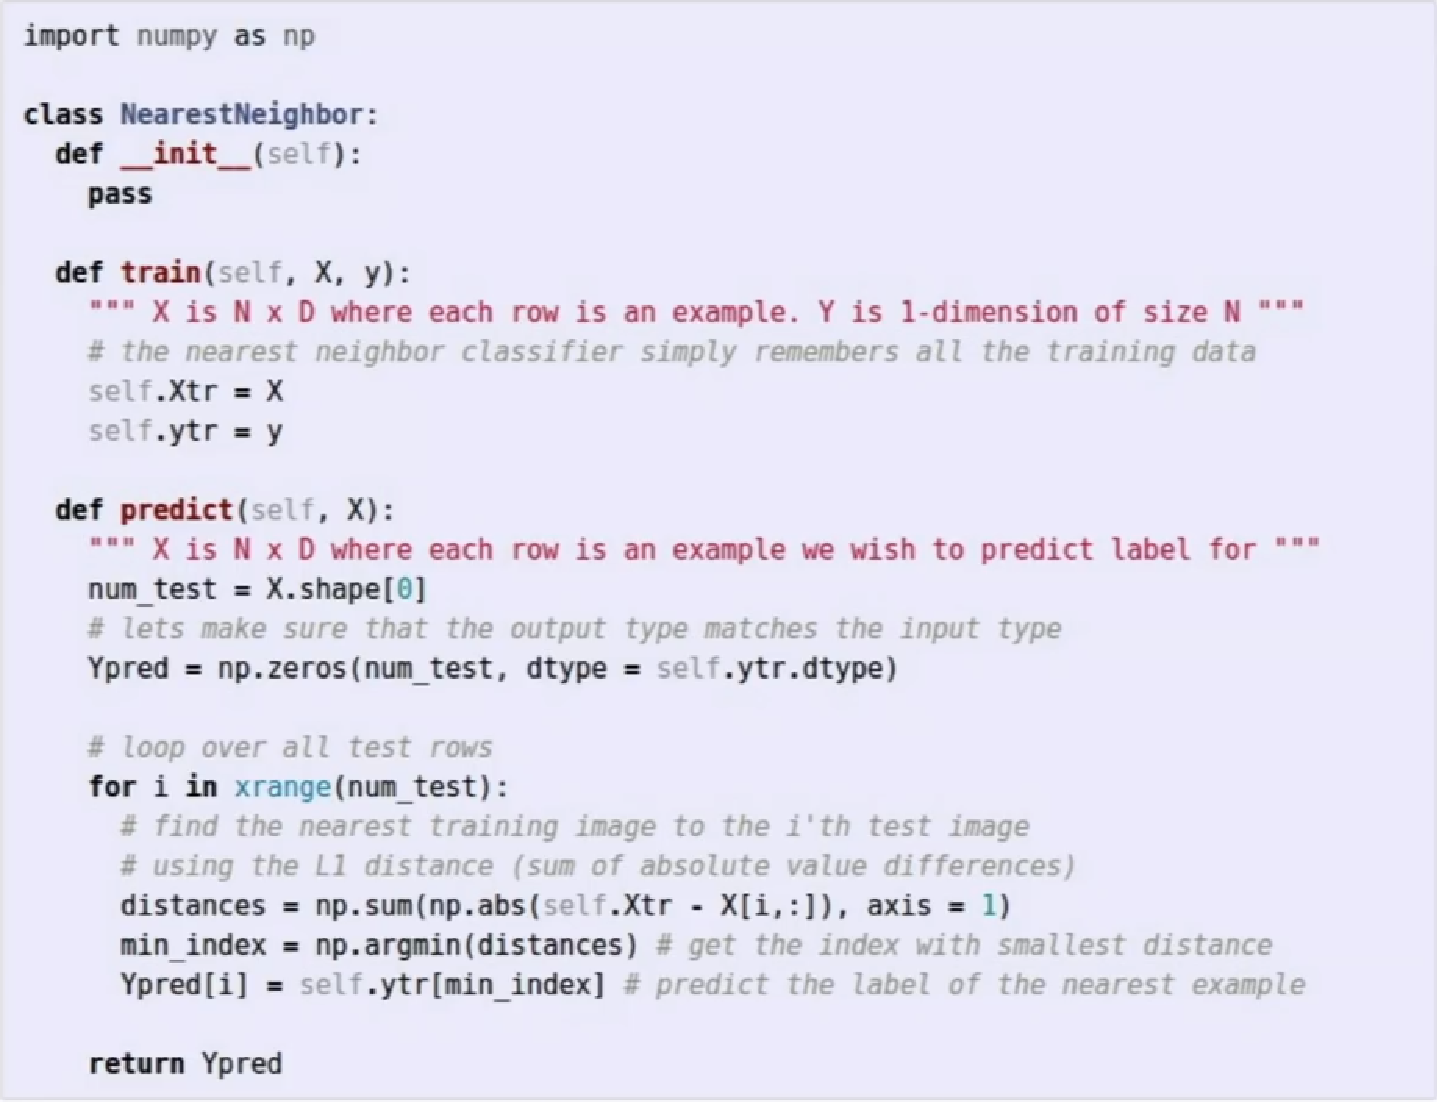
\includegraphics[width=0.75\linewidth]{L1.pdf}
\caption{ Nearest neighbour classifier example}
\label{fig:L1}
\end{figure}
It is preferable to have during a deep learning session \textbf{fast predictions and slow testing} \textit{(since it is done separately}, no constraints on time length). When using \textbf{L1 distance} the nearest neighbor the decision regions lie on a 2D plane: colors represents the classes.
For each pixel the method computes what is the nearest example in the training data and colors the regions  of the corresponding class label.The Classifier has errors: islands of color or fingers of color at the borders.
\paragraph{K-nearest neighbors}
Take a vote among K nearest neighbors \textit{(by selecting a weight or by some pre-determined rules, usually a majority vote) } => solves some problems \textit{(like islands etc.)}
White regions mean that there is no majority \textit{(so  the neighbor can be randomly chosen )}.
\paragraph{Euclidean distance}
Another distance example: Euclidean
\begin{equation}
 d_2(I_1, I_2) = \sqrt{(\Sigma_p (I_1^p - I_2^p)^2) }
\end{equation}{}
It is independent from the coordinates system since it generates a circle.\\\\
Try different \textbf{distance metrics }when approaching to a new problem.

K and the distance metrics are hyperparameters.  The  decisions are taken before programming, they are very problem-dependent.A \textbf{hyperparameter} is a parameter whose value is set before the learning process begins.
\paragraph{Data preparation}
split the data into:
\begin{enumerate}
    \item \textbf{train} to train the algorithm
    \item \textbf{validation} to validate the code and choose and tune the hyperparameters \item \textbf{test} when  running the code on unseen data and accuracy of the model is checked. 
\end{enumerate}{}
For \textbf{small sets of data} the \textbf{training  data }is divided  into \textbf{folds}. One of these can be the \textbf{validation} one to select \textbf{hyperparameters} and the algorithm runs several times, cycling the validation fold through all the remaining ones and then select the best set of hyperparameters. Labels of validation set are only used to check how good the hyperparameters selection is.
Graphs are made to see the most accurate selection of hyperparameters and easily choose between them.\\\\
K-nearest neighbors are never used  due to:
\begin{enumerate}
    \item easy \textbf{errors}
    \item curse of \textbf{dimensionality}:  need for an exponential set of training data to cover the n-D space of pixels
\end{enumerate}{}
\paragraph{Linear Classification}
Neural networks can be made of linear classifiers.
\paragraph{Parametric approach }
The working principle of the parametric Approach is summerized by the following picture \ref{fig:L11}
\begin{figure}[h]
\centering
\captionsetup{justification=centering}
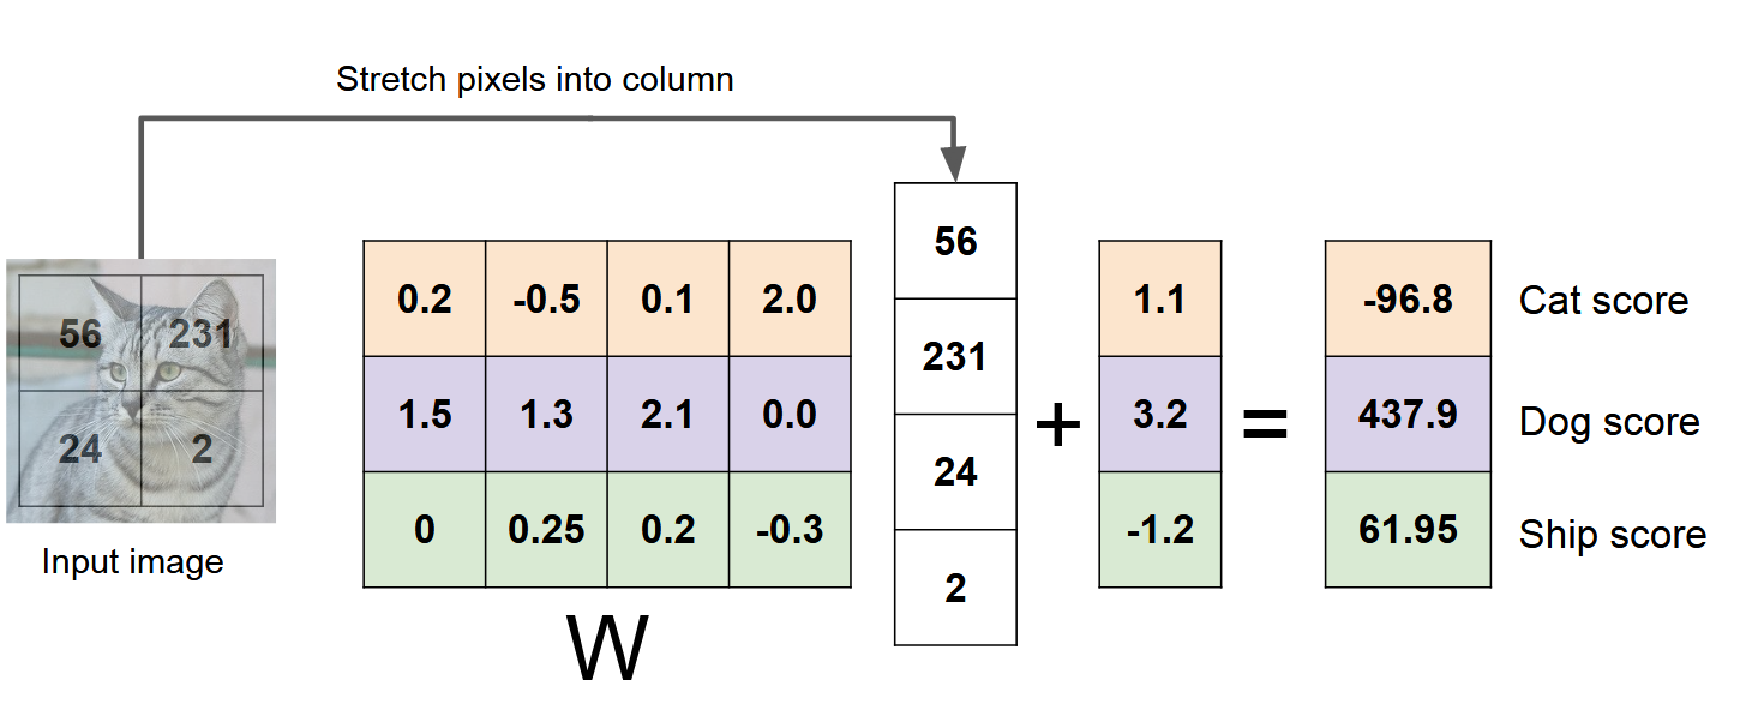
\includegraphics[width=0.75\linewidth]{L11.pdf}
\caption{ Parametric approach}
\label{fig:L11}
\end{figure}\\
The image ,converted into  a vector $\mathbf{x} $, is the input, then it is transformed by  the function $\mathbf{f(x,W)}$ and the result is a class score.
Larger score for a class means that the image will probably belong to that class.\\\\
 
Consider the case of images $32x32x3 (rgb)$.
The Simplest approach is when
\begin{equation}
 \mathbf{f(x,W) = Wx}   
\end{equation}{}
 $\mathbf{f}$ is $10x1$, $\mathbf{W}$ is $10x3072$ and $\mathbf{x}$ Is 3072x1.
If the set is unbalanced, a\textbf{ bias}  term  can be added 
\begin{equation}
 \mathbf{f(x,W) = Wx + b  } 
\end{equation}{}
$\mathbf{b}$ is 10x1.
The output vector will have a \textbf{class score} for each element.
\textbf{Linear classification} is almost a \textbf{template} matching approach \textit{(the template is determined by the weights of each class)}.
If the classifier is trained, the visualization the weight for each class is available. Blurry images of one template for each class will be obtained.
\begin{figure}[h]
\centering
\captionsetup{justification=centering}
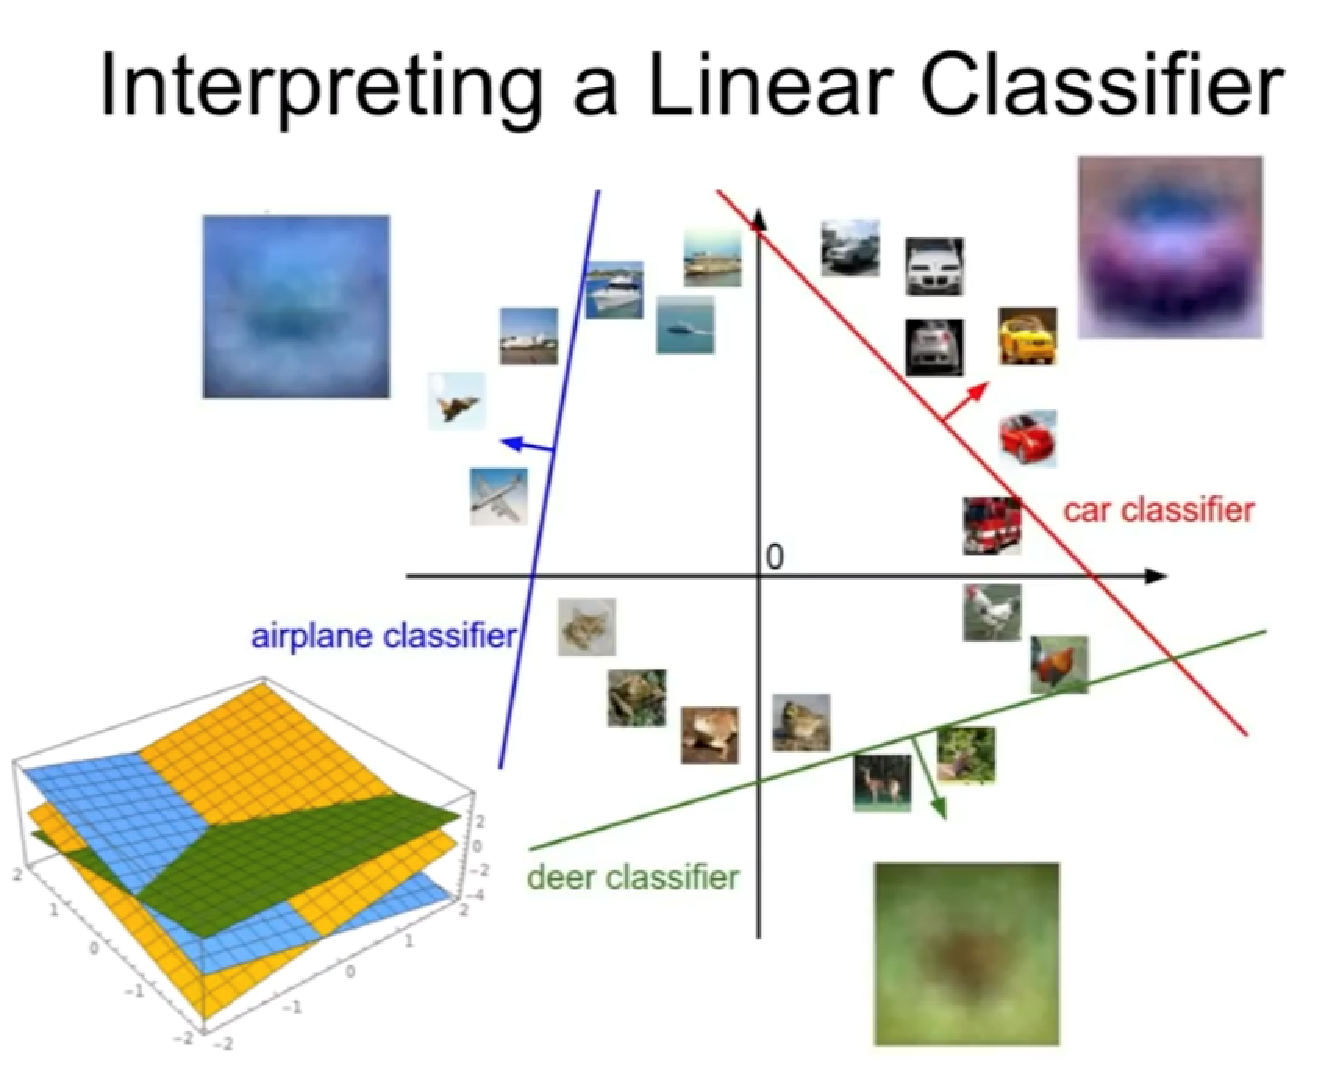
\includegraphics[width=0.75\linewidth]{L12.pdf}
\caption{ Linear classifier}
\label{fig:L12}
\end{figure}\\
There are problematic examples for linear classifiers but it is simple
How is it possible to distinguish whether W is good or bad?








\clearpage
\subsection{Lecture 3 | Loss Functions and Optimization}
\textbf{Youtube link:}\\
\url{https://www.youtube.com/watch?v=h7iBpEHGVNc&list=PL3FW7Lu3i5JvHM8ljYj-zLfQRF3EO8sYv&index=3}\\
\textbf{Slides:}\\
\url{http://cs231n.stanford.edu/slides/2017/cs231n_2017_lecture3.pdf}
\paragraph{How to choose W }
Each row  of the $\mathbf{W }$ matrix  corresponds to a class, and if the row is wrapped into an image matrix the  template blurry images is obtained.
Quantify the badness of  $\mathbf{W }$ to select the best weight: \textbf{Loss function}\\


Imagine to have a training data set: ${(x_i,y_i)}_{I = 1}^N$ where $x_i$  are the pixels of the image and the $y_i$  the values we want the model to predict (labels or targets).
In \textbf{CIFAR-10 } $y_i$ are integers between 1 and 10 or 0 and 9 i.e. one of the 10 labels .
$L_i$ is the loss function that takes the linear classifier function of $x_i$ and $\mathbf{W }$ (predicted scores) and right labels/targets $y_i$. The output is the value that describes how bad the classifier is and the total \textbf{loss function L} is the \textbf{average} on the entire dataset.
\begin{equation}
    L= \frac{1}{N}\sum_{i} L_i (f(x_i,W),y_i)
\end{equation}{}
Search the space of \textbf{W}s that minimize the total Loss function.
\paragraph{Multicass SVM Loss}
First example of loss function:\\
\begin{equation}{}
L_i=  \Sigma_{j \neq y_i}
\begin{cases}
 0  \ \ \ if \ \ \ s_{y_i} >= s_j + 1\\
s_j -s_{y_i} + 1 \ \ \ otherwise
\label{svm}
\end{cases}{}
\end{equation}\\
$s= \mathbf{f(x_i,W)}$ is the predicted score the subs correspond to a particular class
 $j$ are all the wrong classes (cycle) and $y_i$ is the right one, 1 is the safety margin difference between the incorrect score sum and the correct score one.
Then to obtain the total L, make an average of $L_i$.\\
\begin{minipage}{0.5\textwidth}
This loss function is also called \textbf{hinge loss} because of the shape of the graph when it is plotted.
As the score for the correct class increases, the loss will decrease. It will reach zero when the safety margin of 1 is overcome.

\end{minipage}
\begin{minipage}{0.5\textwidth}
\begin{figure} [H]
\centering 
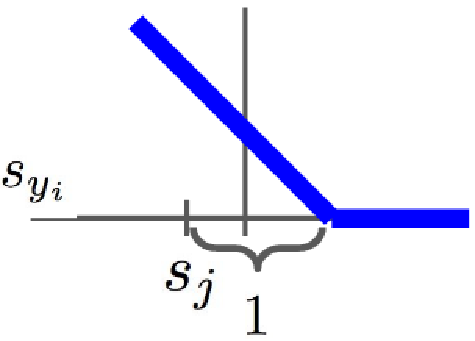
\includegraphics[scale=0.8]{L211.pdf}
\caption{Hinge loss}
\label{fig:L211}
\end{figure}
\end{minipage}\\

\textbf{Square hinge} loss is also used, it is the same as \ref{svm} but with a square of everything after the sum.
If  a square loss is used it will avoid square wrong predictions, and it will distinguish between different kinds of errors \textit{(different importance).}

\clearpage
Multiclass \textbf{SVM} example code:\ref{fig:L212}
\begin{figure}[h]
\centering
\captionsetup{justification=centering}
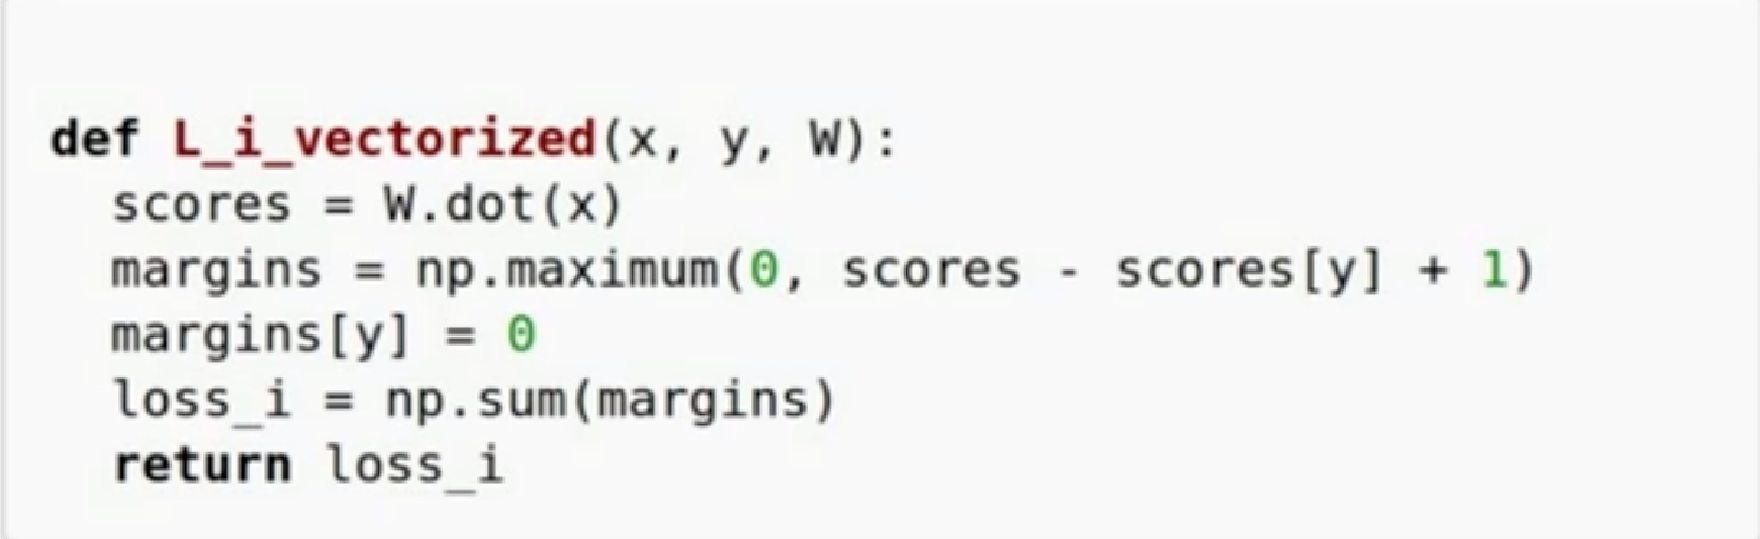
\includegraphics[width=0.75\linewidth]{L212.pdf}
\caption{ \textbf{SVM} example code}
\label{fig:L212}
\end{figure}\\
Take care of the \textbf{performance and Loss on the test data, not of the training one}.\\
The loss function does not have to fit the training data, it will lead to errors or inconvenient loss functions. To simplify the loss function \textit{(i.e. if the loss function is a curvy complicate line, it is better to have regular one, a straight one)}.  There is an term added to the loss function:  $\lambda \textbf{R(W)}$, an explicit regularization penalty. $\lambda$ will be one of the hyperparameters to be tuned during validation data usage.
By this add-on the  function is encouraged the to \textbf{straighten} \textit{(in the case of a polynomial function, but this is valid for other function with different parametrization)}.
\begin{equation}
      L= \frac{1}{N}\sum_{i} L_i (\mathbf{f(x_i,W),y_i})+\lambda R\textbf{(W)}
\end{equation}{}
There are a variety of regularization terms \label{norm}
\begin{enumerate}
    \item One of the most common is the L2 regularization \ \ \   $ R(\mathbf{W}) = \Sigma_k \Sigma_l \mathbf{W}_{k,l}^2$. It measures the complexity of the classifier \textit{(in this case it will spread the $\mathbf{W_i}$ across all the vector).}
      \item L1 regularization \ \ \   $ R(\mathbf{W}) = \Sigma_k \Sigma_l |\mathbf{W}_{k,l}|$.  It has a different conception of complexity \textit{(in this case the number of zeros in the weight matrix/vector)}.
\end{enumerate}{}
\begin{figure}[h]
\centering
\captionsetup{justification=centering}
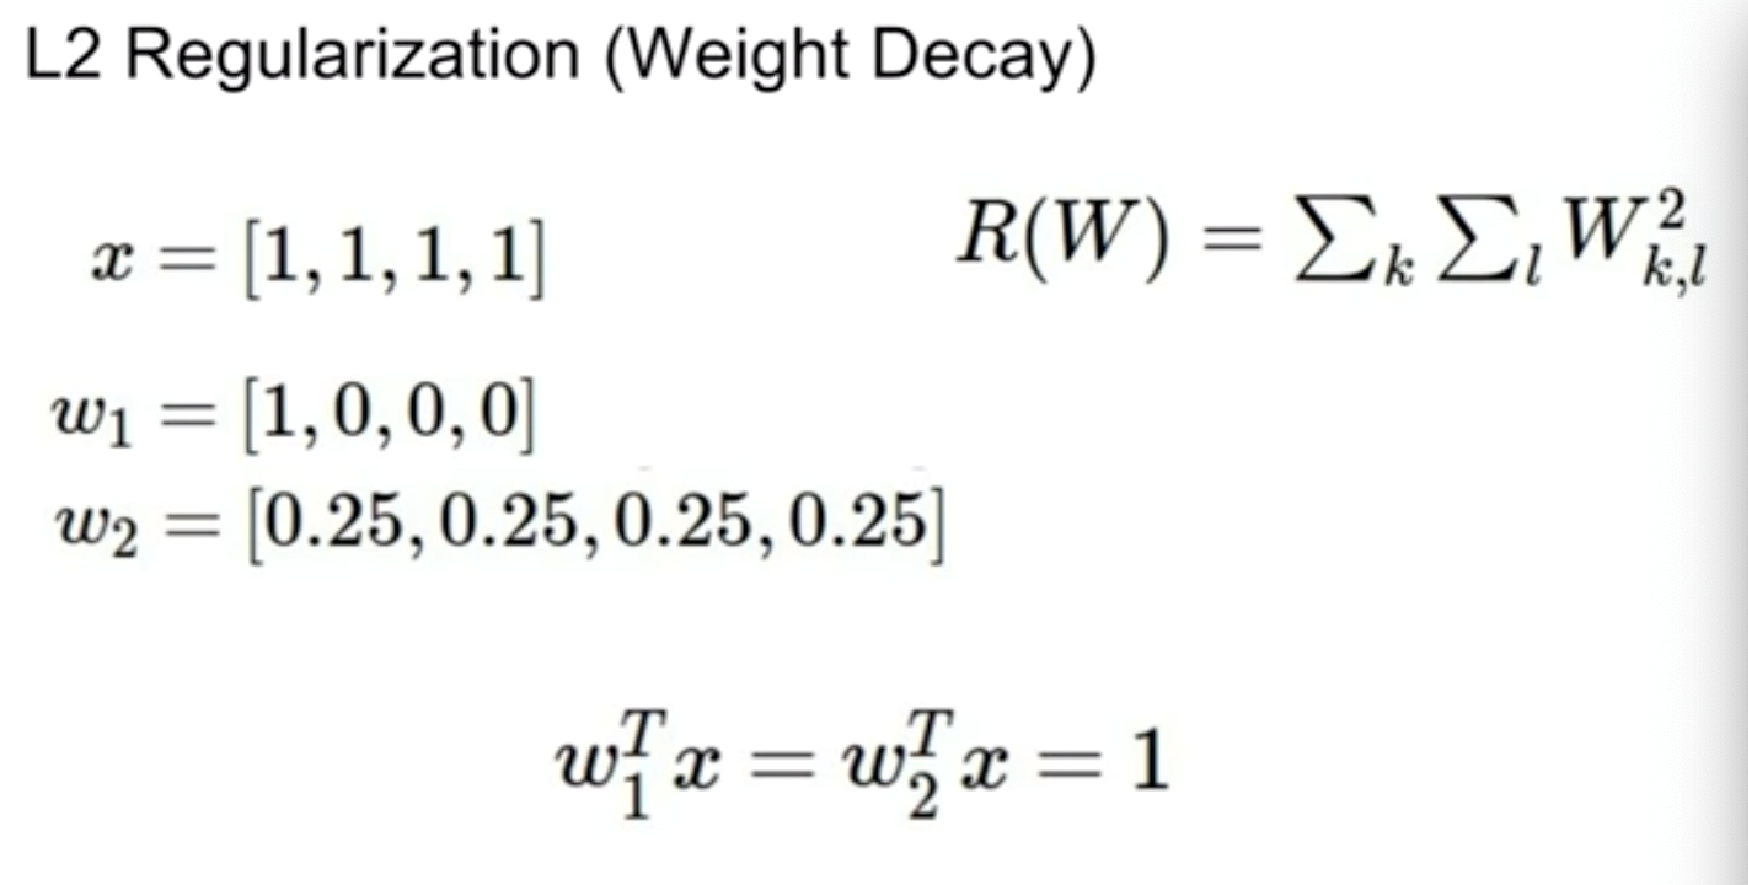
\includegraphics[width=0.75\linewidth]{L213.pdf}
\caption{ $L_2$ regularization effect}
\label{fig:L213}
\end{figure}
\clearpage

\paragraph{Softmax classifier}
\begin{figure}[h]
\centering
\captionsetup{justification=centering}
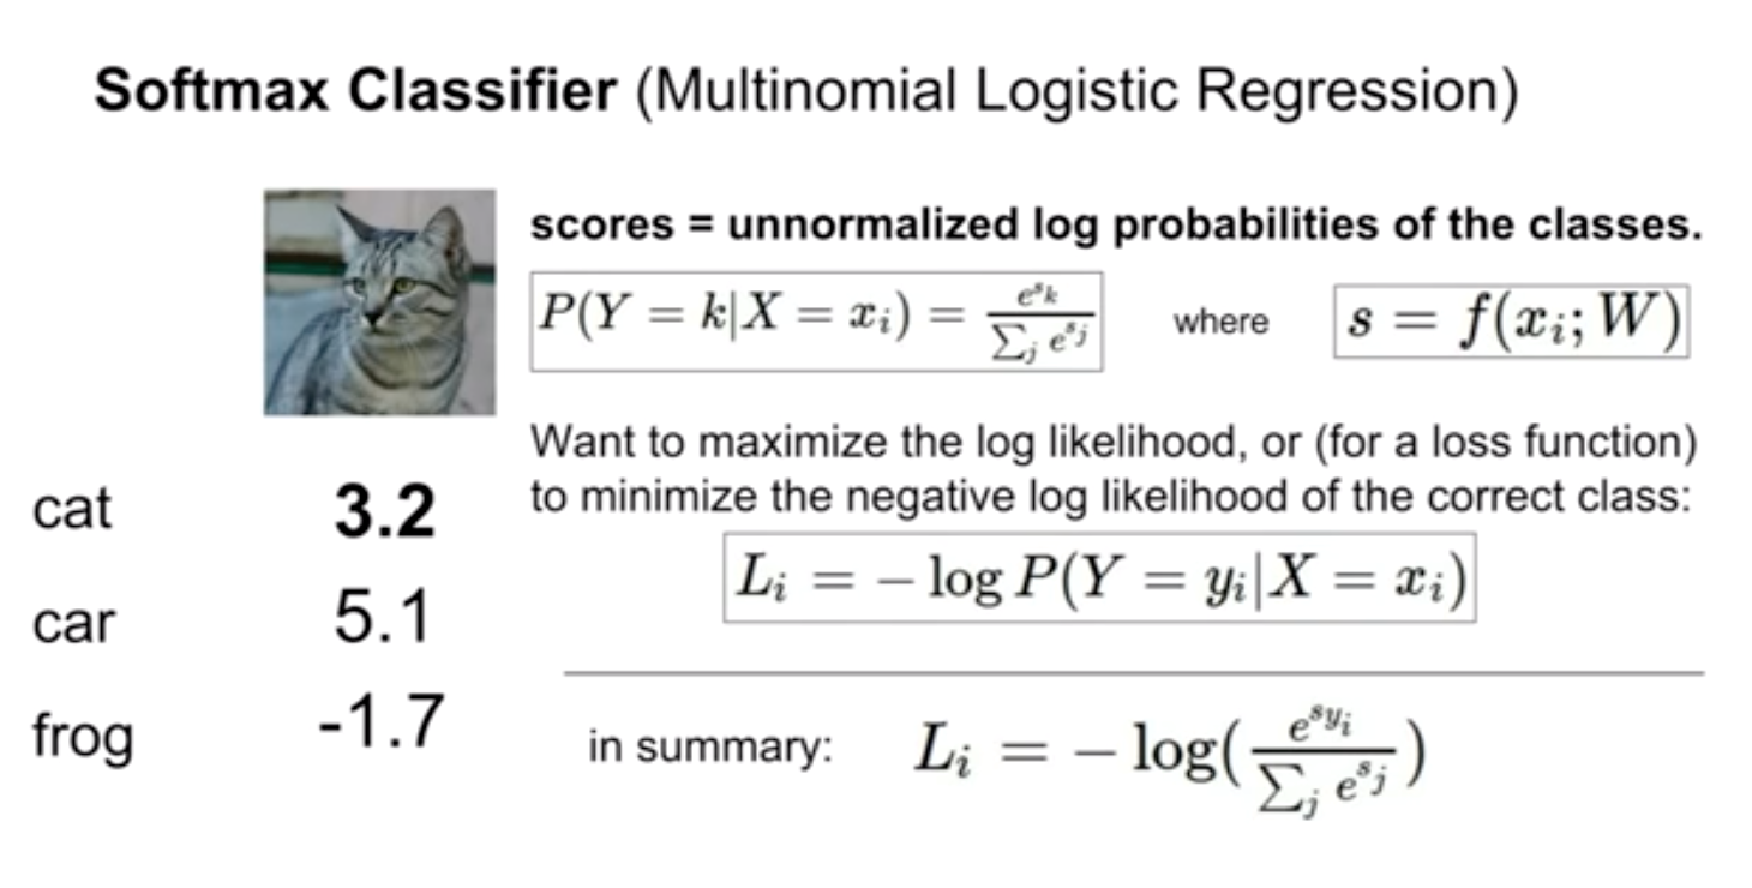
\includegraphics[width=0.75\linewidth]{L214.pdf}
\caption{ Softmax classifier}
\label{fig:L214}
\end{figure}
The ratio on the left of \ref{fig:L214} is called \textbf{Softmax function.}
A\textbf{ minus} is added on the $L_i $ function to \textbf{minimize the loss} since the aim is to maximize the probability of the right class \textit{(as near to 1 as possible)}. The procedure is the following:\ref{fig:L215}
\begin{figure}[h]
\centering
\captionsetup{justification=centering}
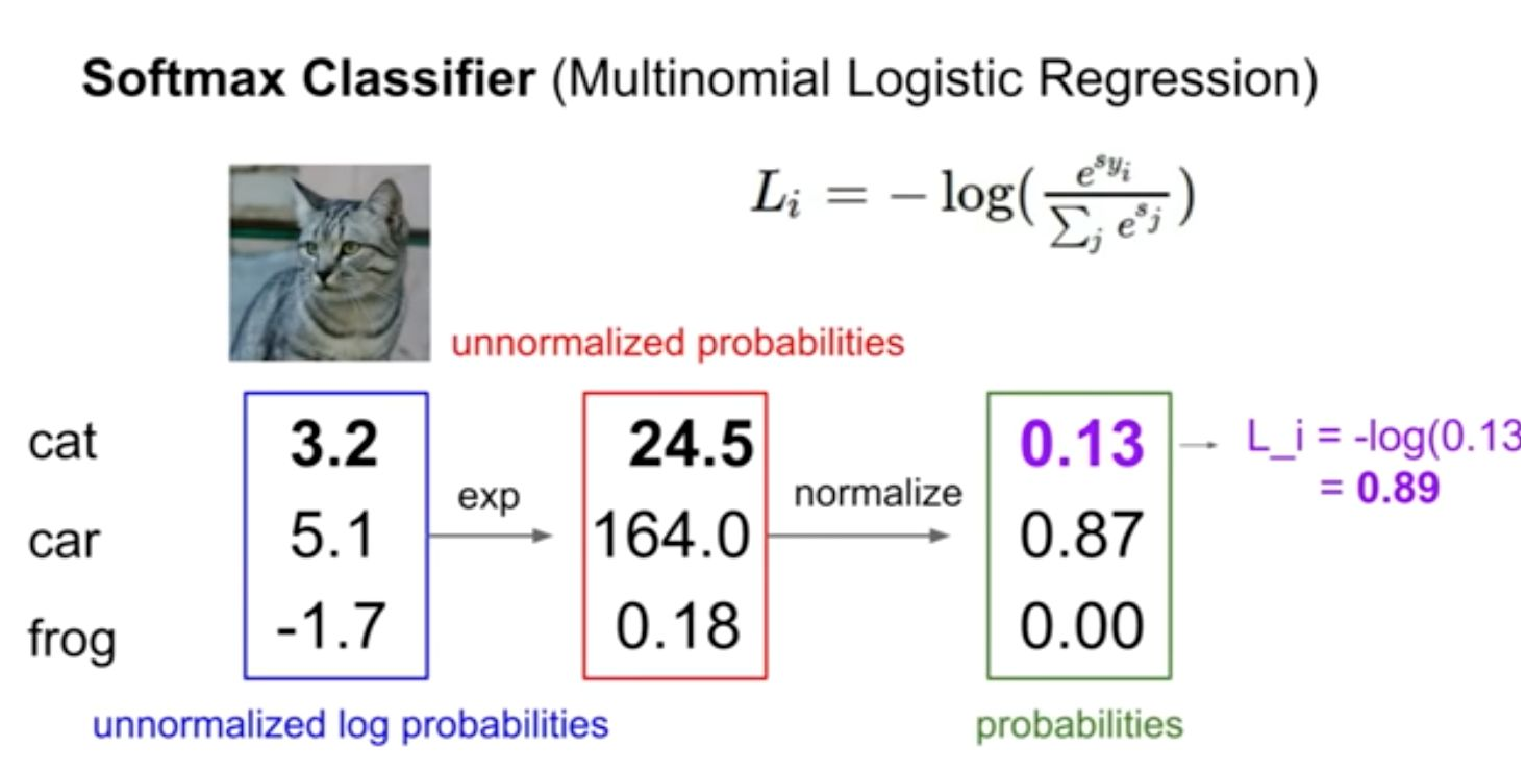
\includegraphics[width=0.75\linewidth]{L215.pdf}
\caption{ Softmax classifier}
\label{fig:L215}
\end{figure}
\paragraph{Differences between softmax and SVM losses:}
\begin{itemize}
    \item \textbf{Softmax} always wants to drive probability of the correct class to one, so even there is a high score on the correct class and low scores on the wrong ones, it will always pile up weight on the correct score. It Continuously improves \textit{(minimize)} the loss value.
    \item In the \textbf{SVM} loss if  the scores are modified, due to the threshold \textit{(set usually to 1 )},  would not probably  make the loss value change.
\end{itemize}{}
\clearpage
\begin{figure}[h]
\centering
\captionsetup{justification=centering}
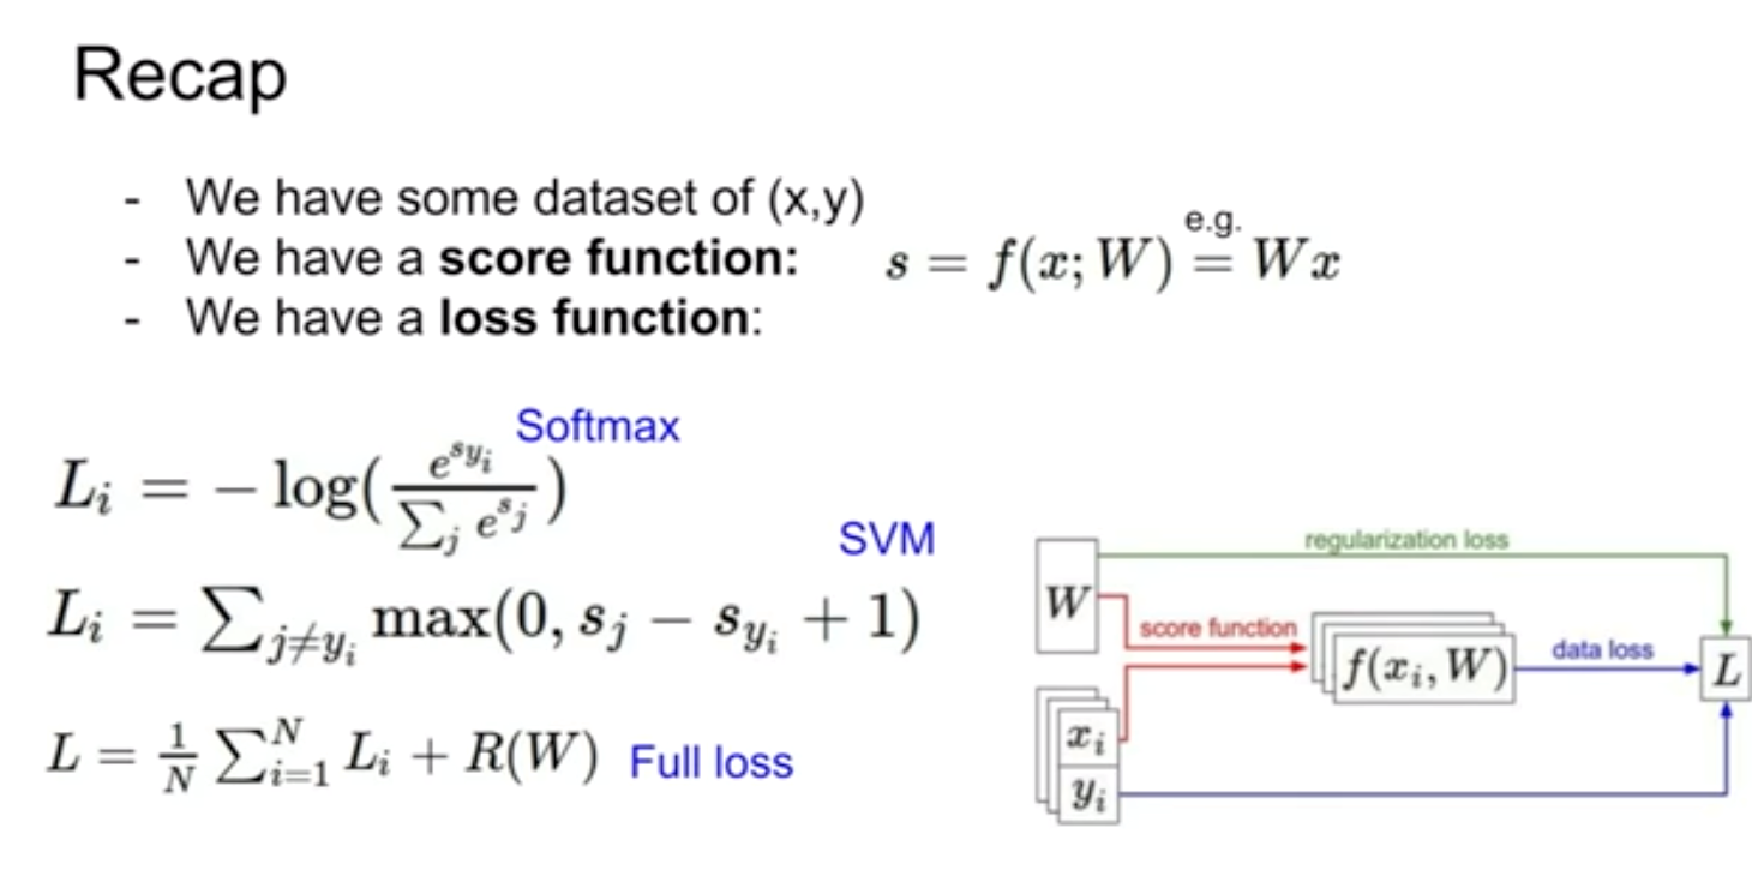
\includegraphics[width=0.75\linewidth]{L216.pdf}
\caption{ Recap on \textbf{SVM} Softmax and Full Loss}
\label{fig:L216}
\end{figure}

\paragraph{Optimization}
\begin{enumerate}
    \item	Based on \textbf{gradients}, using iterative methods like \textbf{finite differences} \textit{(super slow solution, terrible idea, but used as a debugging tool)}

\item	Use calculus to compute \textbf{analytic gradient}, faster, usually exact \textit{(error prone)}

\item	Simple three line algorithm:

\end{enumerate}{}
\begin{figure}[h]
\centering
\captionsetup{justification=centering}
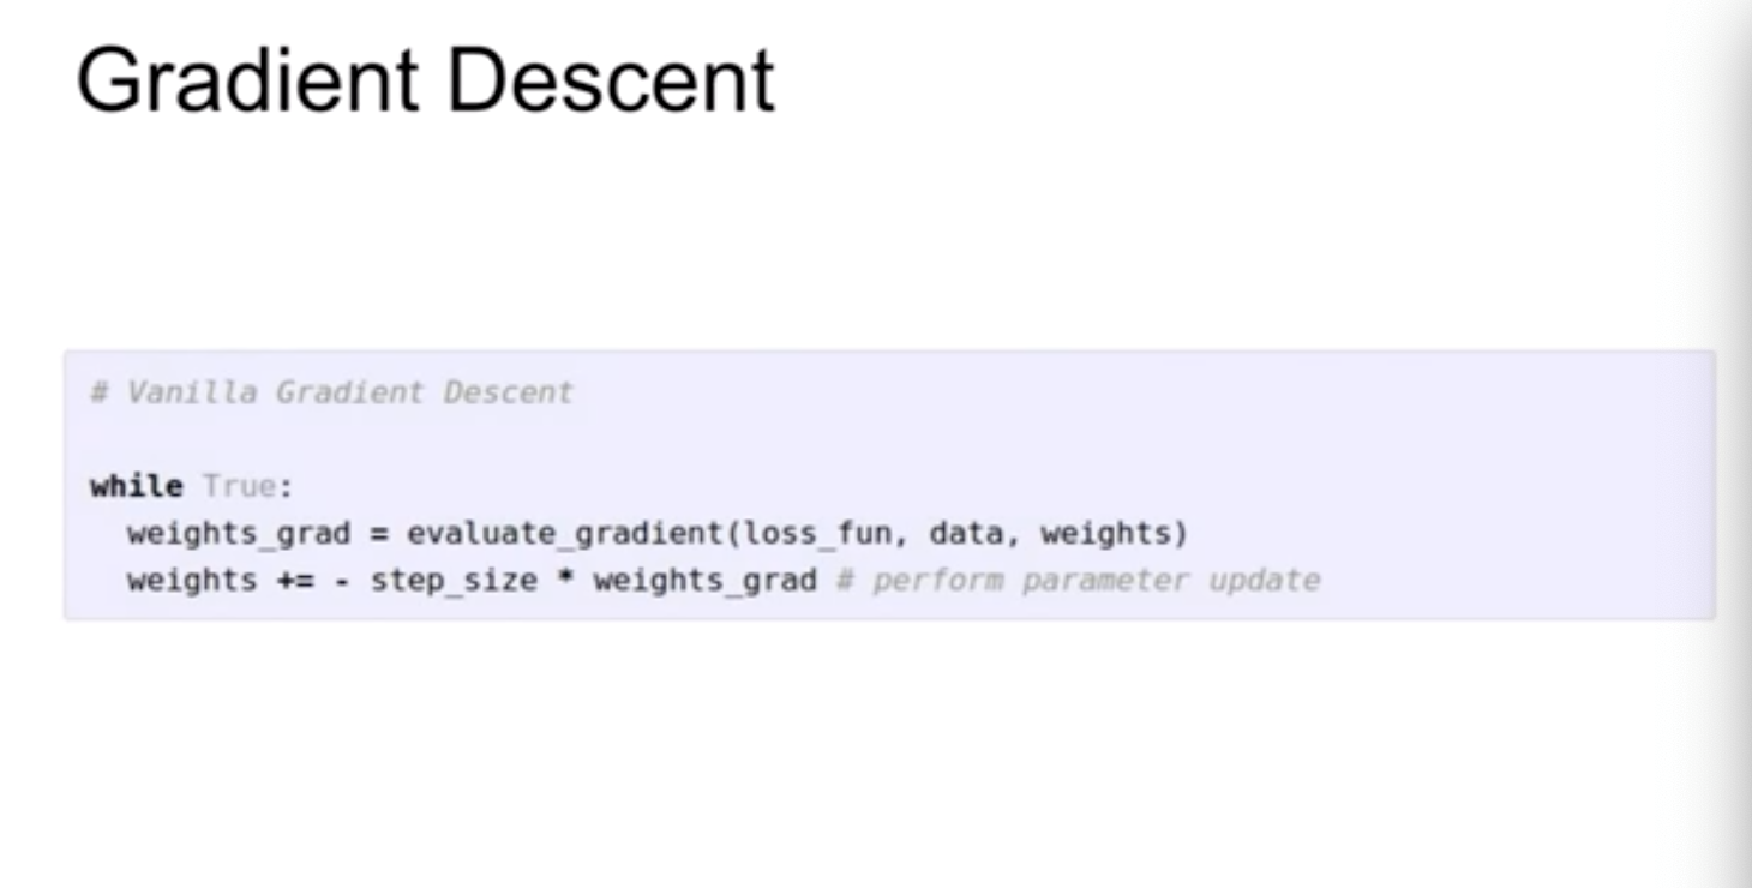
\includegraphics[width=0.75\linewidth]{L217.pdf}
\caption{ Gradient descent}
\label{fig:L217}
\end{figure}
The \textbf{stepsize} is an \textbf{hypermparameter}, first one to check \textit{(learning rate)}.
\paragraph{Stochastic gradient descent}
The number N of data available could be countless. As a matter of fact computing the loss and the gradients is expensive. The solution is to use  a minibatch of examples as follows \ref{fig:L218}:
\clearpage
\begin{figure}[h]
\centering
\captionsetup{justification=centering}
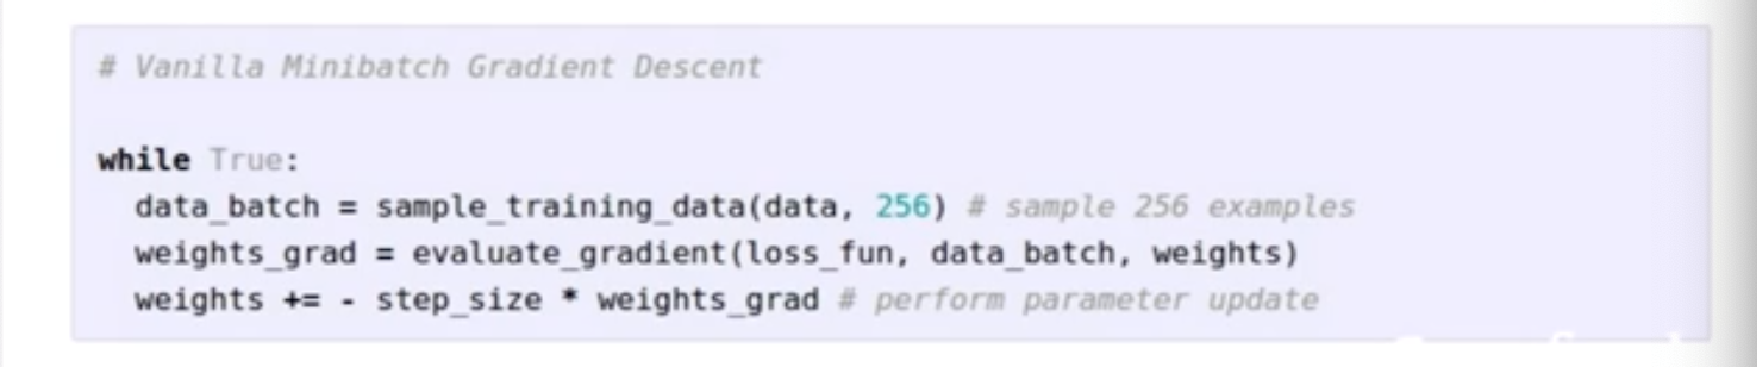
\includegraphics[width=0.75\linewidth]{L218.pdf}
\caption{ Gradient descent code}
\label{fig:L218}
\end{figure}
\paragraph{Image features}
A representation  of an image may be done thanks to \textbf{features} and passed to the \textbf{linear classifier instead of the raw image}.
Find the right \textbf{feature} is significant to make them separable by the linear classifier. Example: divide the spectrum in pockets and calculate the number of pixels in each pocket, to differentiate images according to colors contained.
\begin{figure}[h]
\centering
\captionsetup{justification=centering}
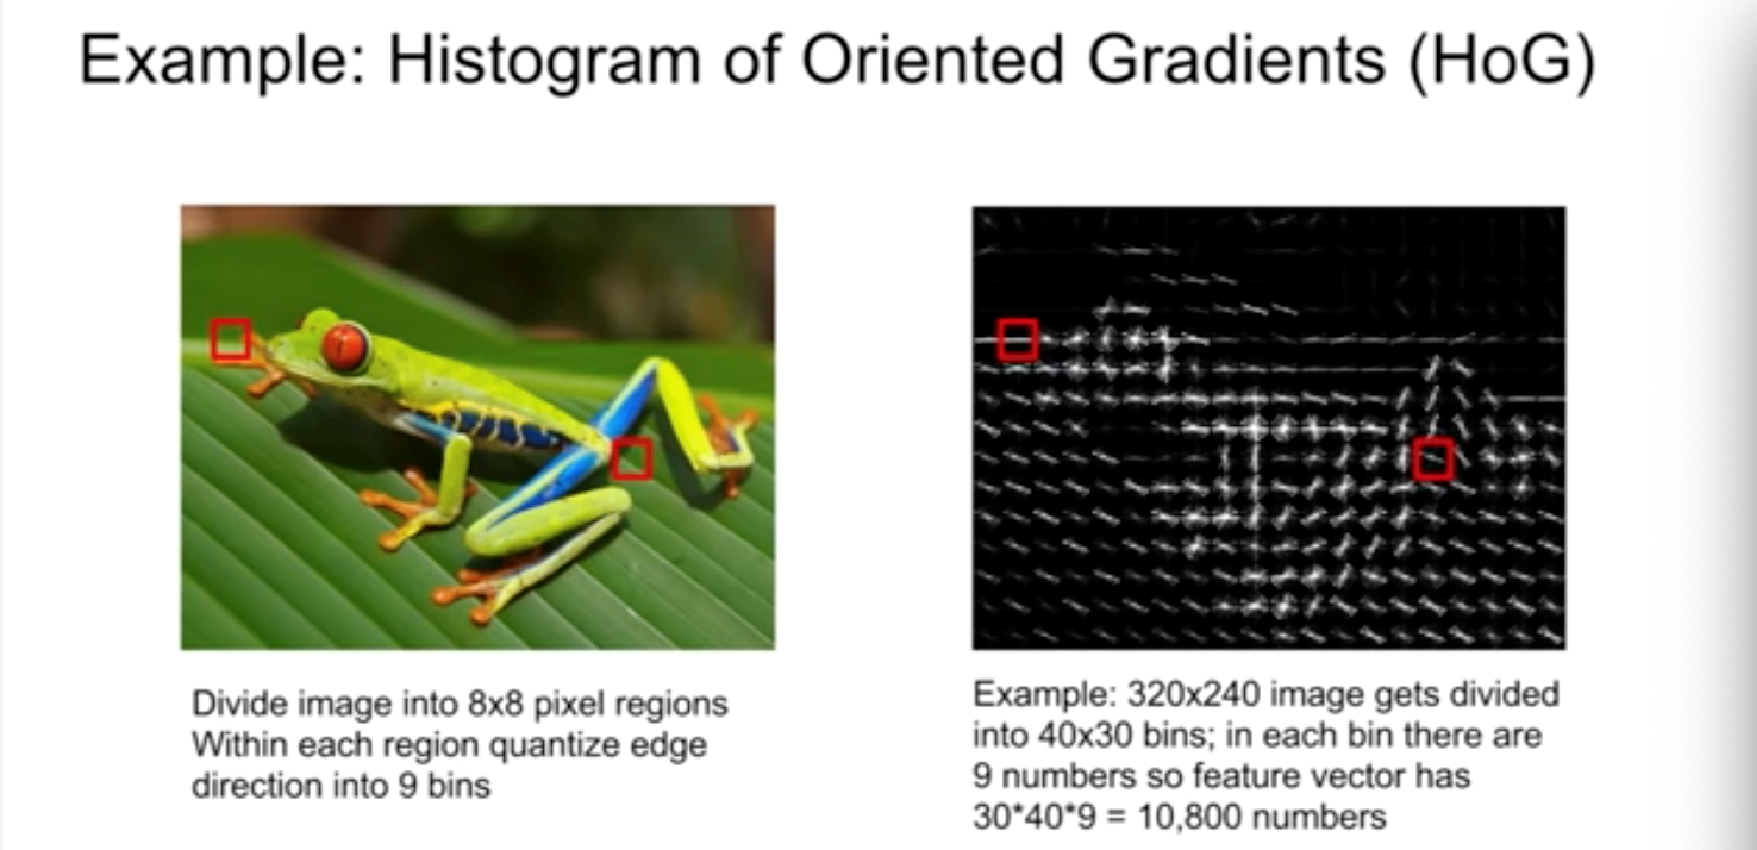
\includegraphics[width=0.7\linewidth]{L219.pdf}
\caption{ Histogram of oriented gradients}
\label{fig:L219}
\end{figure}
\clearpage
Another example could be \ref{fig:L220}
  \begin{figure}[h]
\centering
\captionsetup{justification=centering}
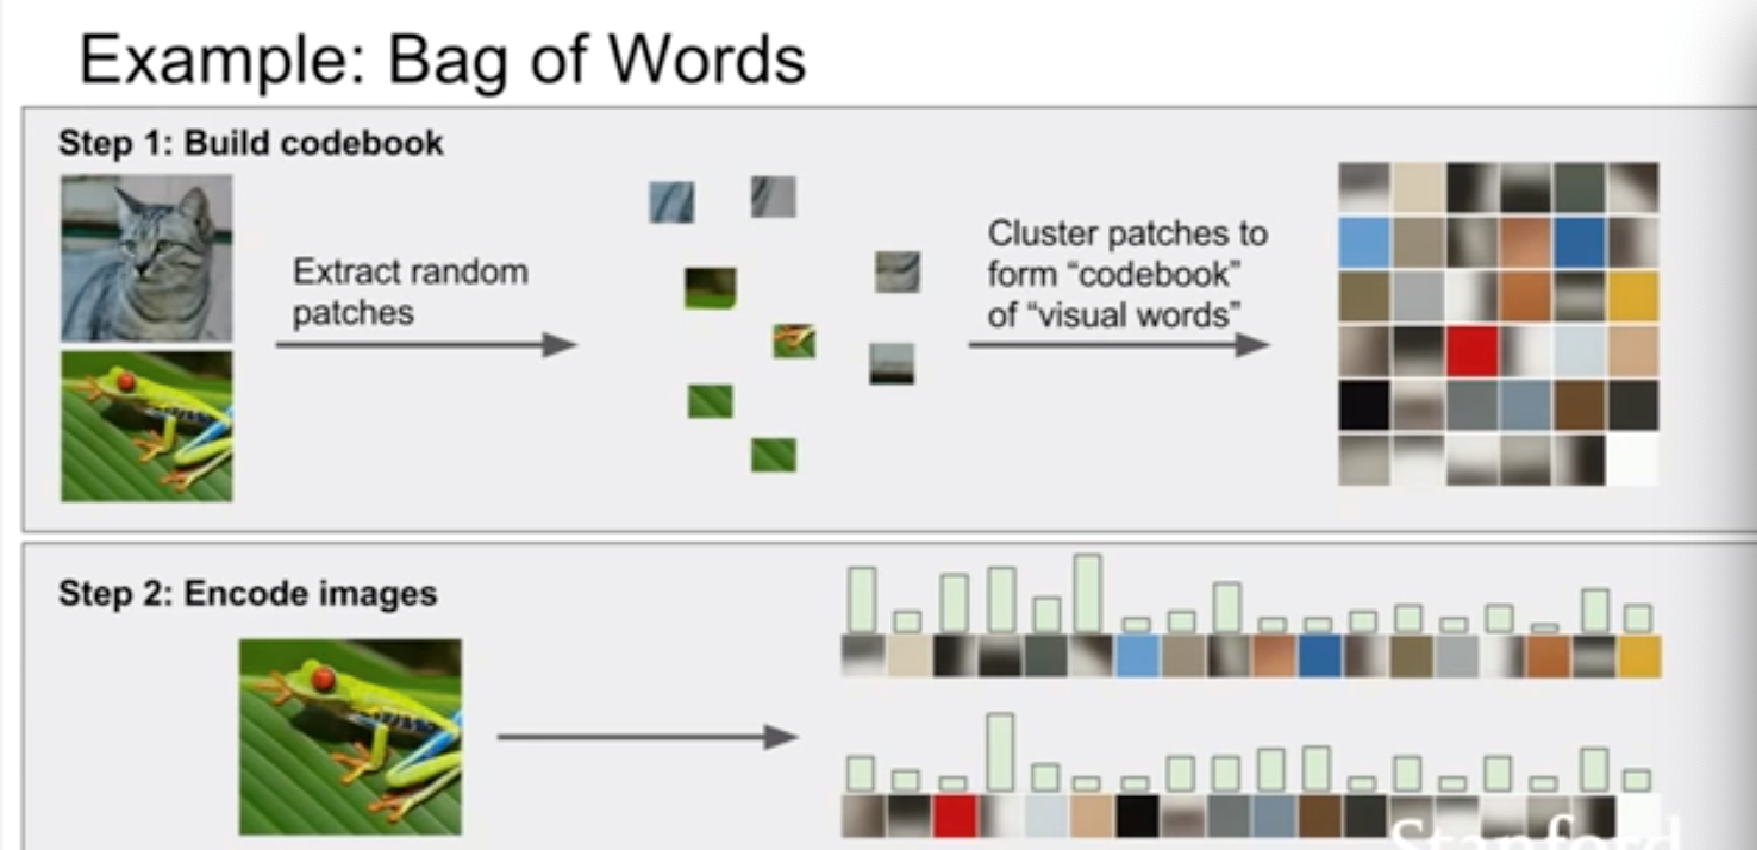
\includegraphics[width=0.7\linewidth]{L220.pdf}
\caption{ Bag of words}
\label{fig:L220}
\end{figure}





\clearpage
\subsection{Lecture 4 | Introduction to Neural Networks}
\textbf{Youtube link:}\\
\url{https://www.youtube.com/watch?v=d14TUNcbn1k&list=PL3FW7Lu3i5JvHM8ljYj-zLfQRF3EO8sYv&index=4}\\
\textbf{Slides:}\\
\url{http://cs231n.stanford.edu/slides/2017/cs231n_2017_lecture4.pdf}
\paragraph{Back propagation}
The  starting point to compute the \textbf{gradients} is from \textbf{the end of a computational scheme},  till the gradient of the function is expressed with respect  all of its \textbf{independent variables} \textit{(use chain rule, multiplying gradients, if necessary)}.\\
\begin{figure}[h]
\centering
\captionsetup{justification=centering}
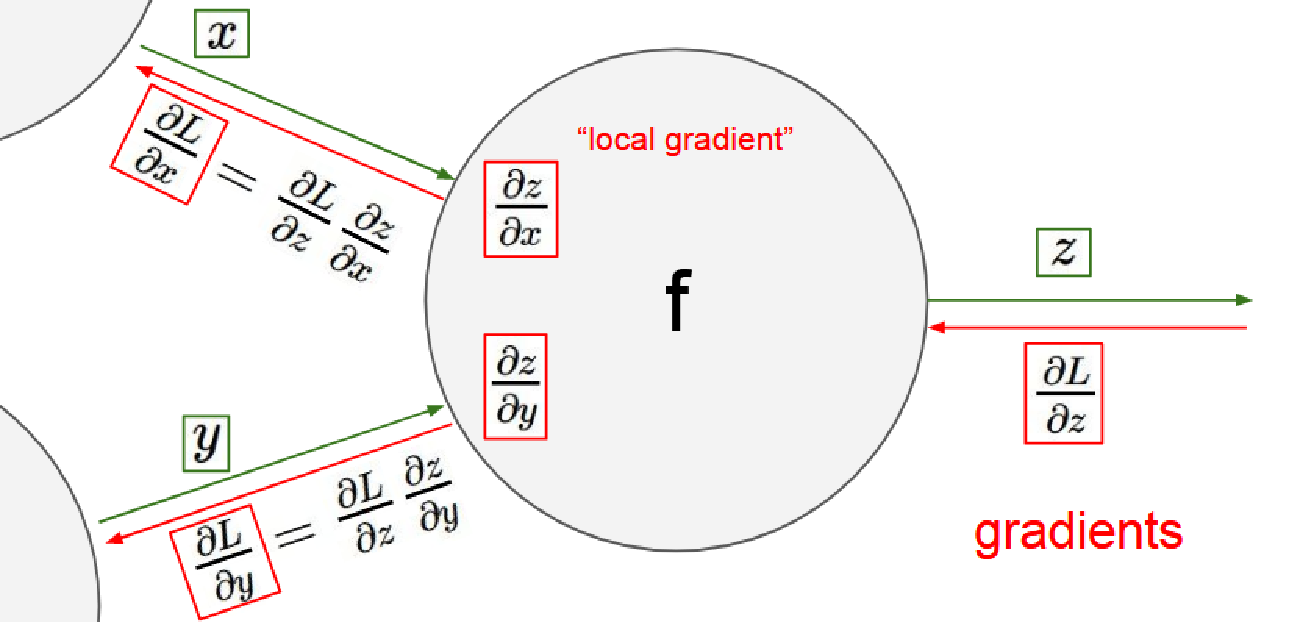
\includegraphics[width=0.7\linewidth]{L310.pdf}
\caption{ Gradient computational graph}
\label{fig:L310}
\end{figure}\\
The \textbf{granulation of the computational graph} is arbitrary, according to how much math you want to do to make it smaller. Here is reported a simple numerical scalar  example \ref{fig:L311}:
\begin{figure}[h]
\centering
\captionsetup{justification=centering}
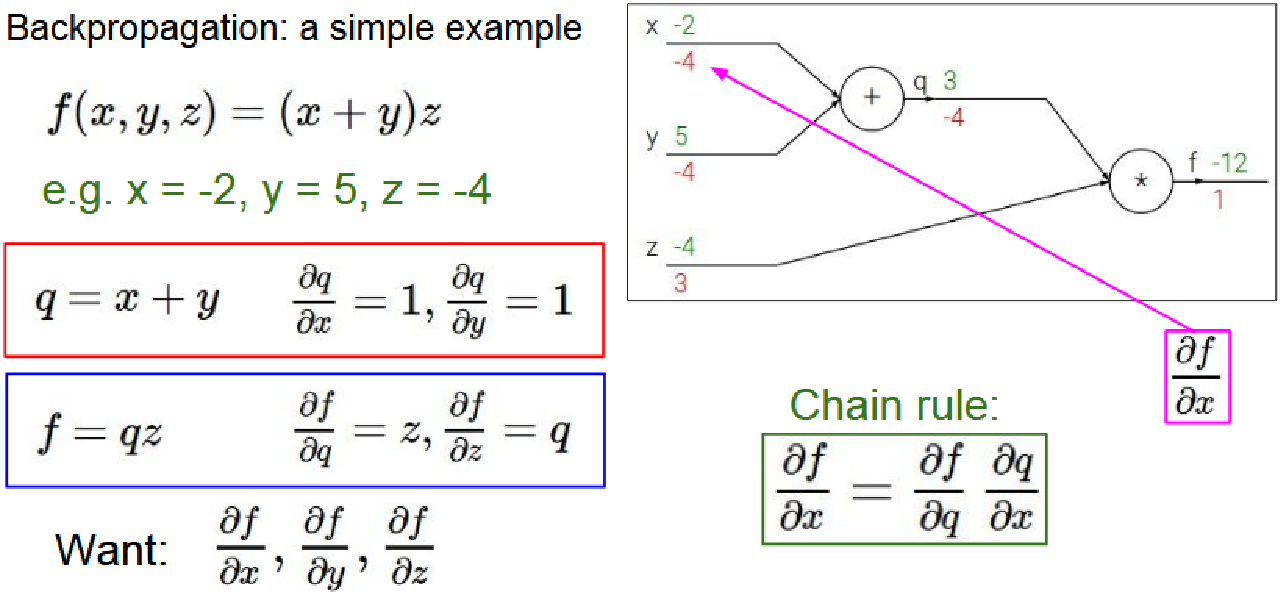
\includegraphics[width=0.7\linewidth]{L311.pdf}
\caption{ A simple Gradient computational graph}
\label{fig:L311}
\end{figure}\\
The underlying idea is in order to get the gradient in a particular position of the graph, starting from the end compute the gradient with respect to the \textbf{local variable} and multiply by the gradient of the \textbf{previous node already calculated}. In this way    $\frac{\partial f}{\partial x},\frac{\partial f}{\partial y},\frac{\partial f}{\partial z}$, are directly expressed as a function of $x,y,z$.

Instead dealing with multidimensional problems in the computational graph \textbf{pay attention to the relative dimensions of tensors} during the back propagation.
\begin{figure}[h]
\centering
\captionsetup{justification=centering}
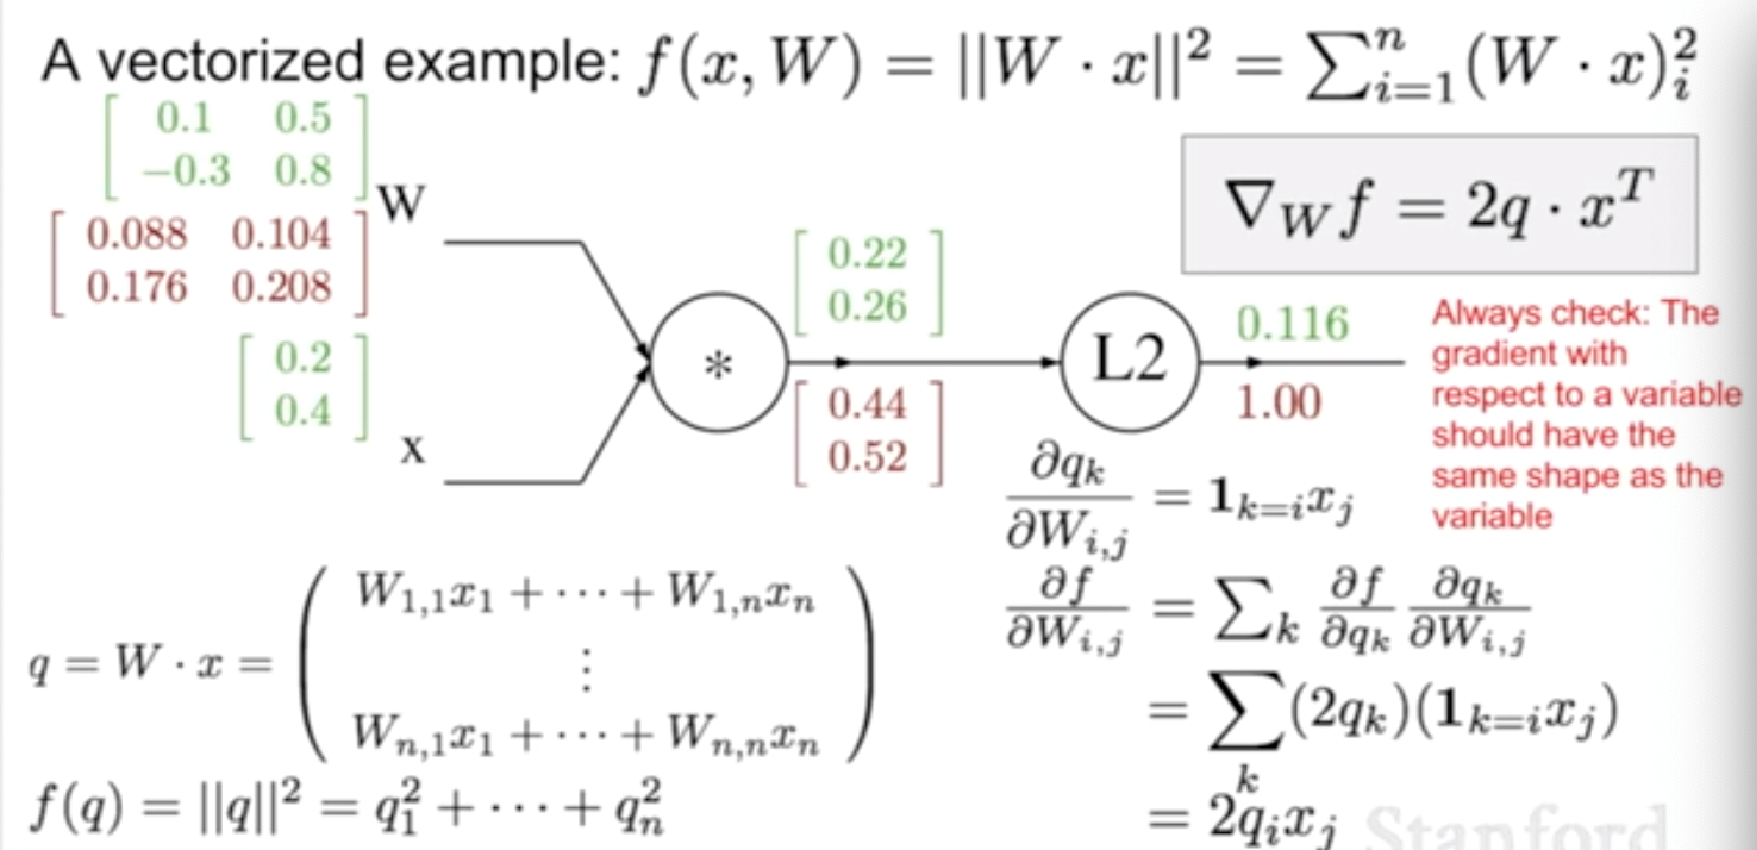
\includegraphics[width=0.7\linewidth]{L312.pdf}
\caption{ A simple gradient computational graph in the vectorized case}
\label{fig:L312}
\end{figure}

Few rules to bear in mind :

\begin{enumerate}
    \item \textbf{Add gate} = gradient distributor
    \item \textbf{Max gate} = gradient router
    \item \textbf{Mul gate} = gradient Switch
\end{enumerate}{}
Obviously all these passages in a computer environment are done by the processor unit. 
Here is shown the relative python code \ref{fig:L313}
\begin{figure}[h]
\centering
\captionsetup{justification=centering}
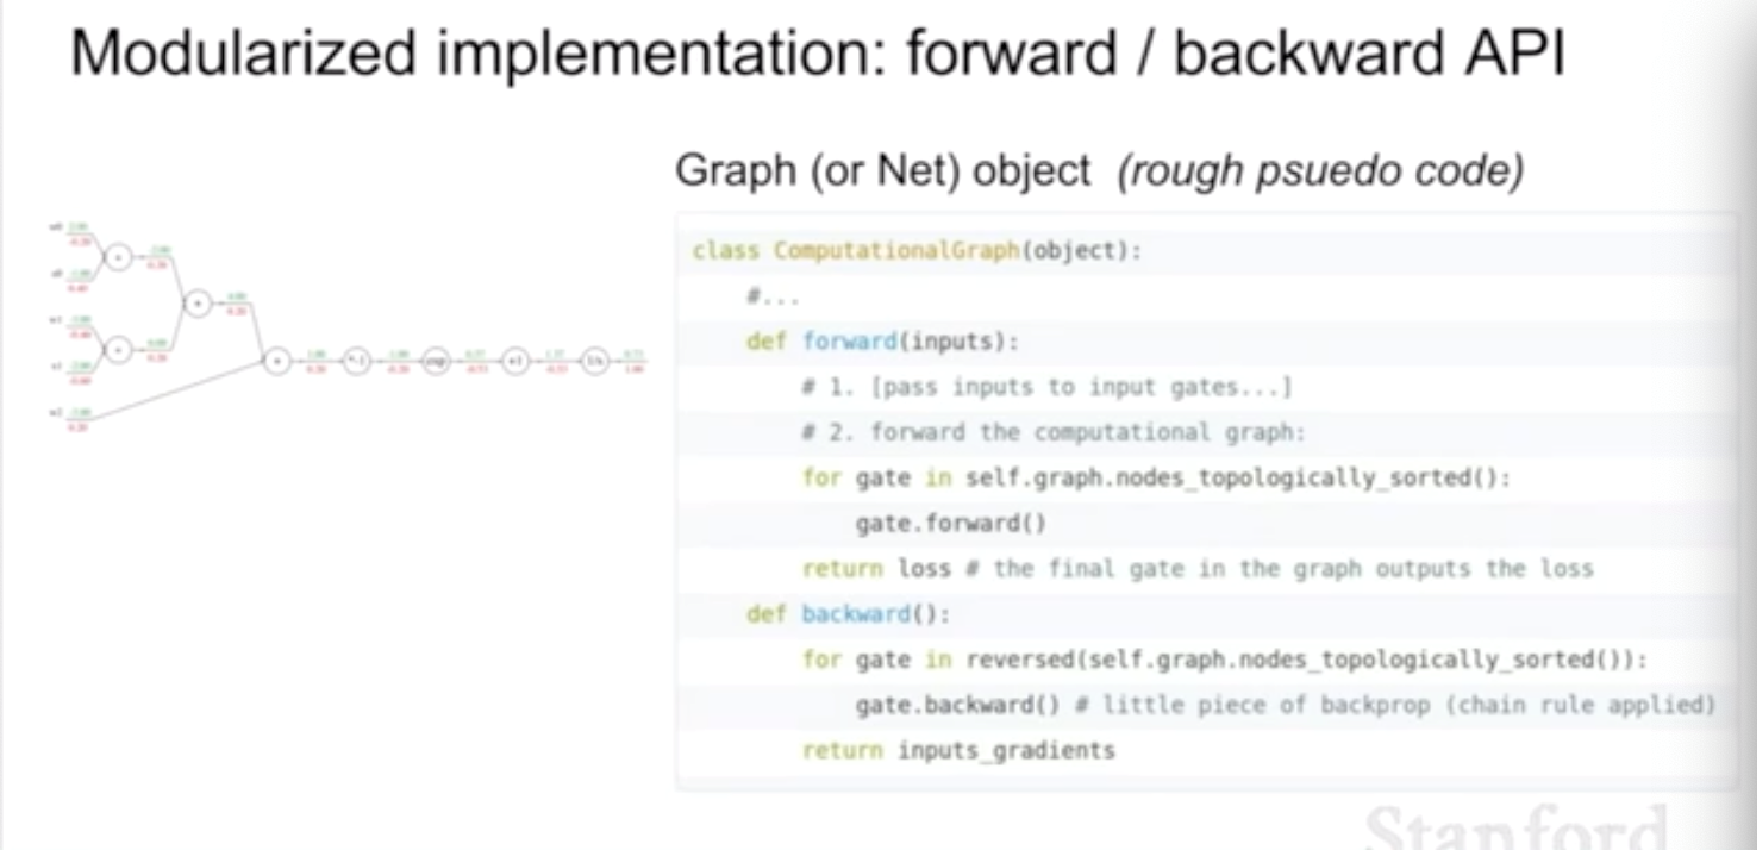
\includegraphics[width=1\linewidth]{L313.pdf}
\caption{ Python code of a gradient computational }
\label{fig:L313}
\end{figure}
\clearpage
\begin{figure}[h]
\centering
\captionsetup{justification=centering}
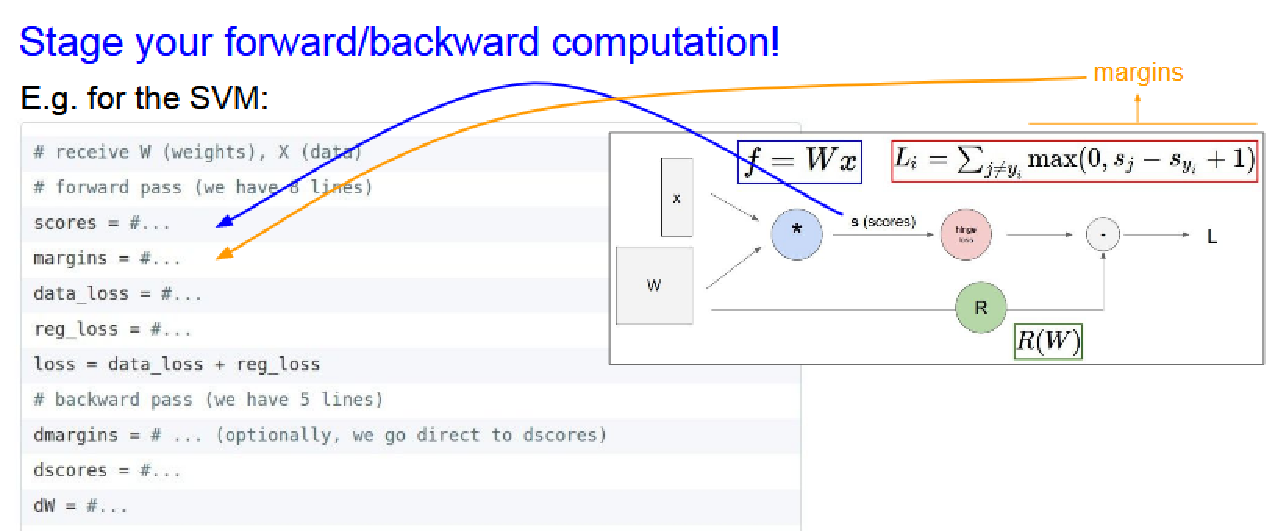
\includegraphics[width=1\linewidth]{L314.pdf}
\caption{ Forward and backward computation}
\label{fig:L314}
\end{figure}
\paragraph{Neural Network}
Example of 2 layer neural network: 
\begin{equation}
   \mathbf{f} = \mathbf{W_2 }max(\mathbf{0, W_1 x)} 
\end{equation}{}
Dealing with multiple layers corresponds to \textbf{superposition} of linear layers.
Non linear functions may be adopted  between this superposition. As said each row of \textbf{W} (weight) is a class template, only one though
,with multiple layer network,  can be combined templates of the same class. Lots of non linear functions are implemented to connect  stack of  layers.
More than 2 layers can be stacked in the same way, and make it become a \textbf{\textquotesingle \textquotesingle deep\textquotesingle \textquotesingle neural network}.
\clearpage
\paragraph{Neuron}
\begin{figure}[h]
\centering
\captionsetup{justification=centering}
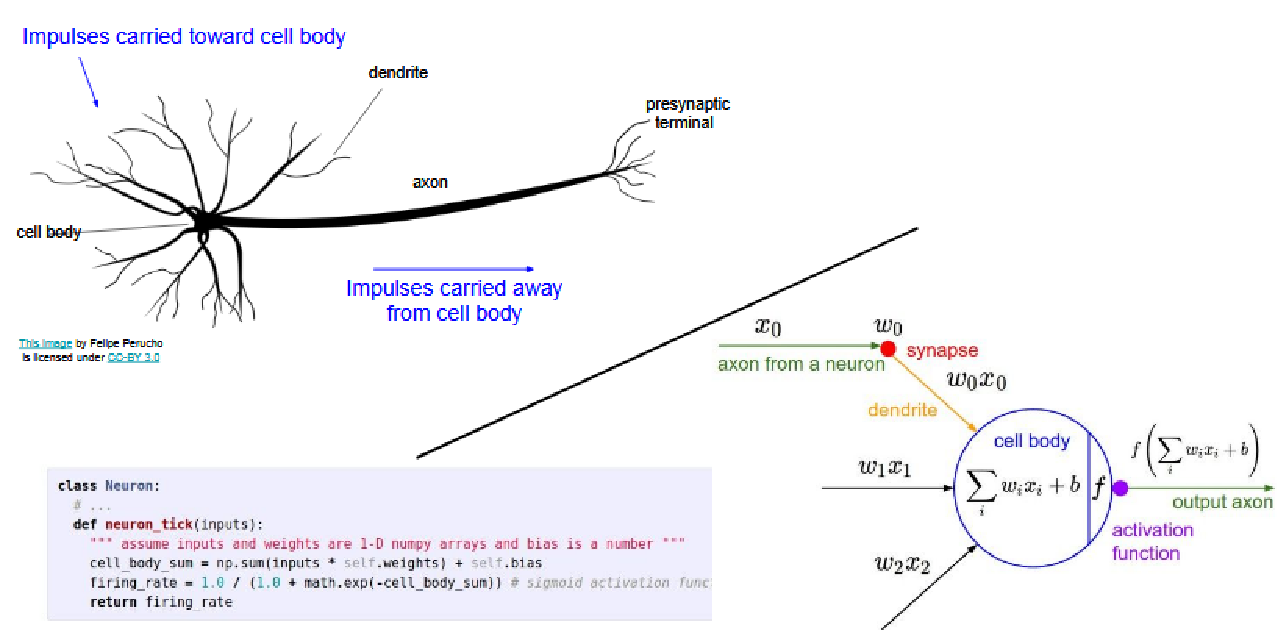
\includegraphics[width=1\linewidth]{L315.pdf}
\caption{ Equivalence between a node and  a neuron}
\label{fig:L315}
\end{figure}

Each node in a network is depicted as a \textbf{neuron}. In a simplistic manner a \textbf{neuron}
\begin{enumerate}
    \item takes in \textbf{input data}
    \item Dendrites perform complex computations
    \item \textbf{Synapses} are not a single weight but a \textbf{complex non linear dynamical system}
    \item The output then is transmitted to the \textbf{following nodes}
\end{enumerate}{}
The \textbf{activation functions}, which outlines how a neuron in network works, are \ref{fig:L316}:
\begin{figure}[h]
\centering
\captionsetup{justification=centering}
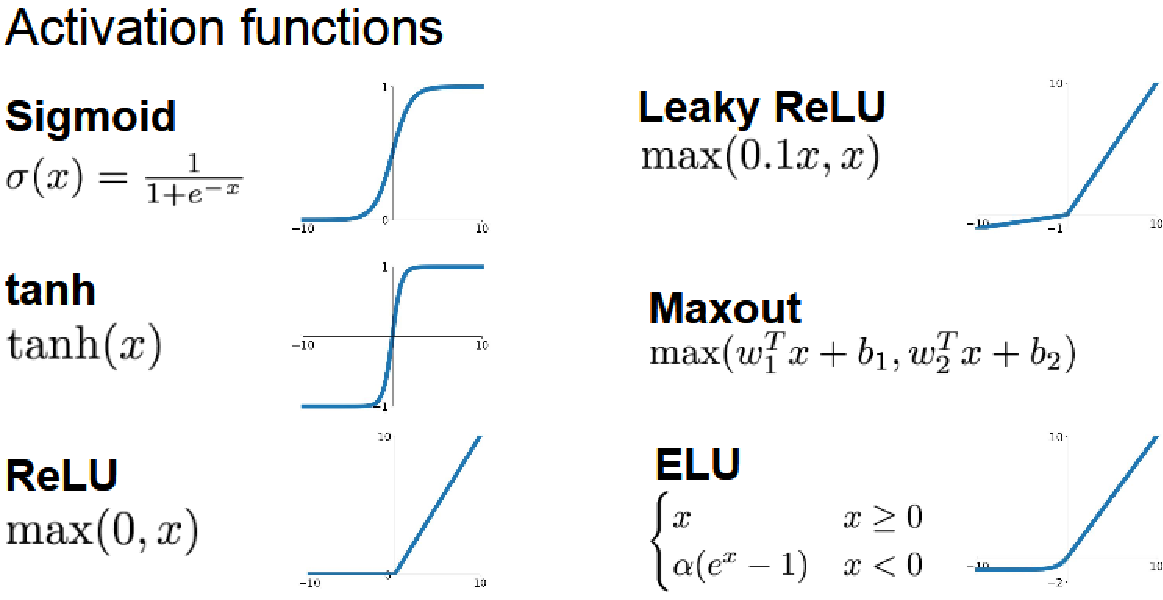
\includegraphics[width=0.7\linewidth]{L316.pdf}
\caption{ Activation functions}
\label{fig:L316}
\end{figure}
\clearpage
Eventually a \textbf{fully connected layer} \textit{(where the nodes or neurons of a single layer are fully connected with the ones of the previous and the ones of the following layer)} is portrayed as \ref{fig:L317}:
\begin{figure}[h]
\centering
\captionsetup{justification=centering}
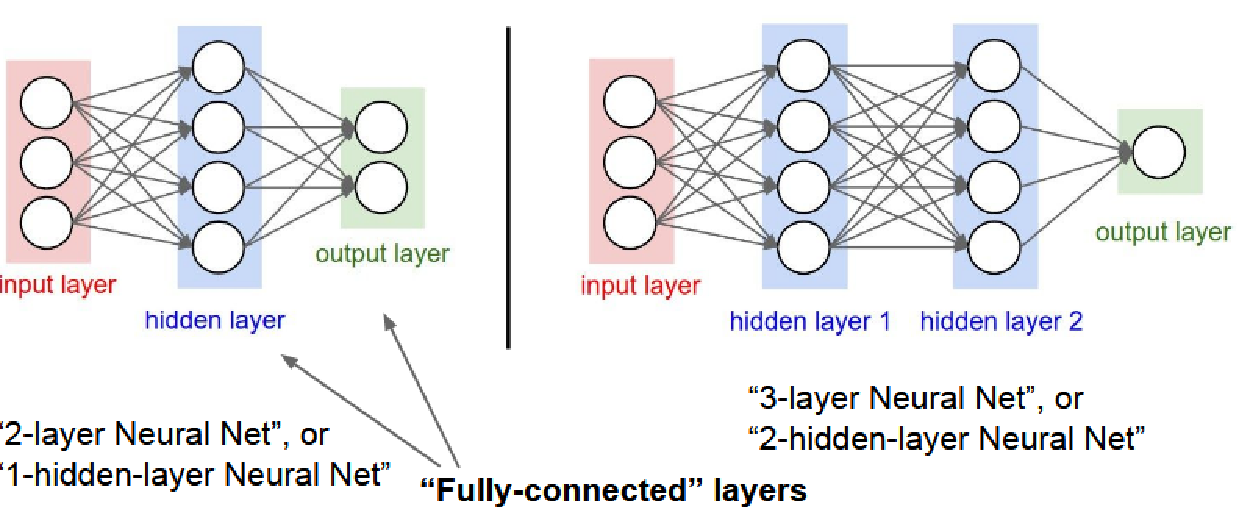
\includegraphics[width=0.7\linewidth]{L317.pdf}
\caption{ Fully connected Networks}
\label{fig:L317}
\end{figure}


\clearpage
\subsection{Lecture 5 | Convolutional Neural Networks}
\textbf{Youtube link:}\\
\url{https://www.youtube.com/watch?v=bNb2fEVKeEo&list=PL3FW7Lu3i5JvHM8ljYj-zLfQRF3EO8sYv&index=5}\\
\textbf{Slides:}\\
\url{http://cs231n.stanford.edu/slides/2017/cs231n_2017_lecture5.pdf}

\paragraph{CNNs}

As seen in the previous lecture, in \textbf{fully connected networks}, all the nodes are completely connected from one layer to next one. This kind of structure is sustainable when dealing with \textbf{not complex problems}, where the dimension of \textbf{W} is relatively small across the layers.
\textbf{CNNs} instead, since being \textbf{partially connected}, can operate with more challenging problems.
In \textbf{convolutional layers}  three dimensional inputs are not unwrapped: The spatial structure is preserved. 
A filter is convolved  with the image \textit{(slide over the image spatially, computing dot products)} and a bias term is added \ref{fig:L410}, producing an \textbf{activation map}.\\
\begin{minipage}{0.5\textwidth}
\begin{figure} [H]
\centering 
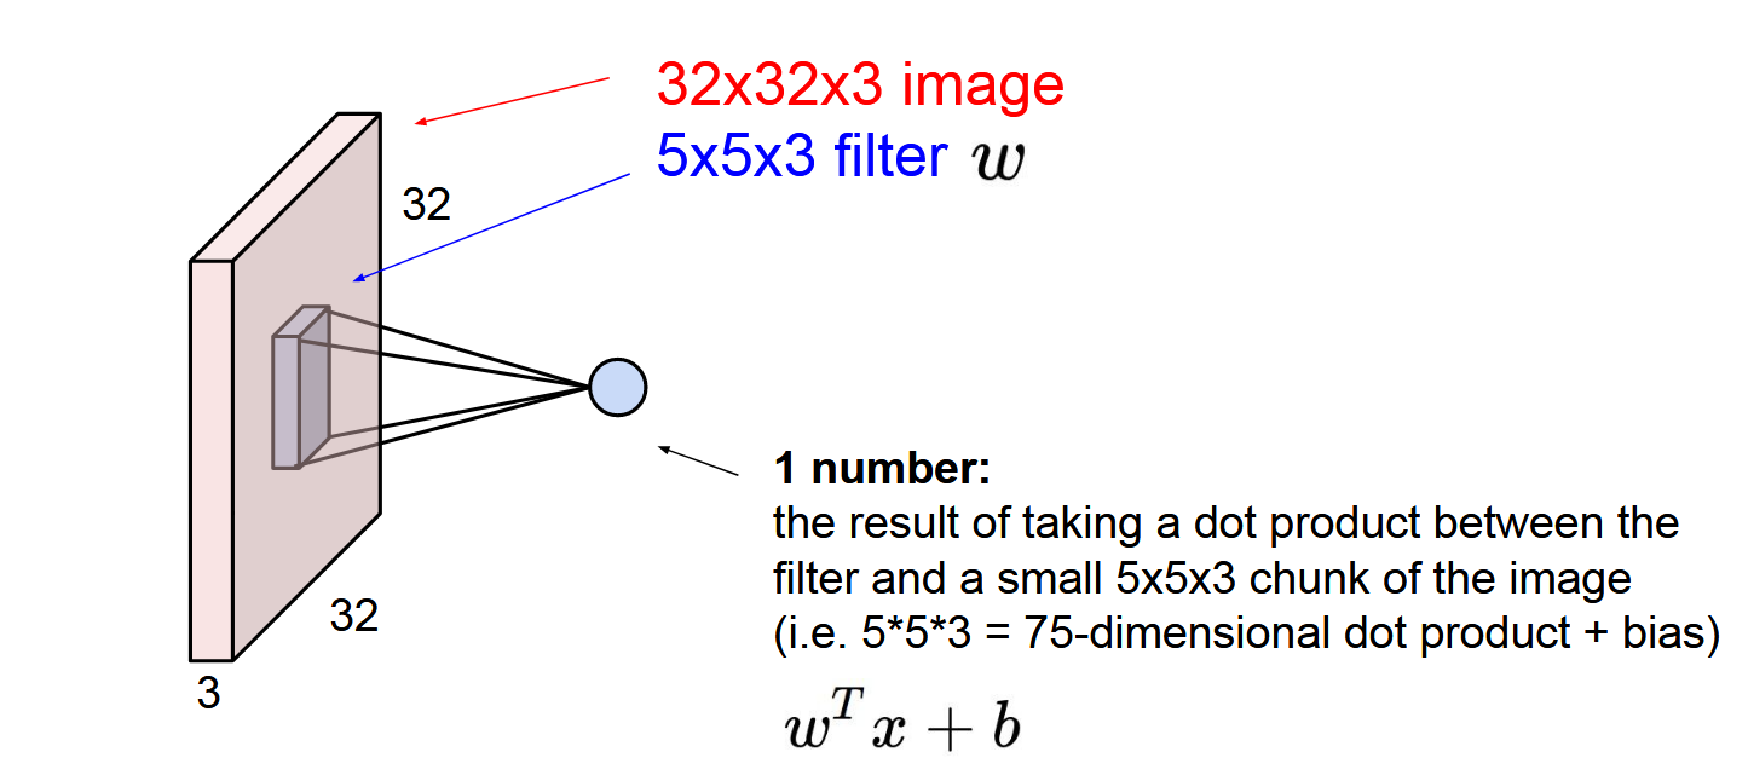
\includegraphics[scale=0.28]{L410.pdf}
\caption{ filter on a \textbf{CNN}}
\label{fig:L410}
\end{figure}
\end{minipage}
\begin{minipage}{0.5\textwidth}
\begin{figure} [H]
\centering 
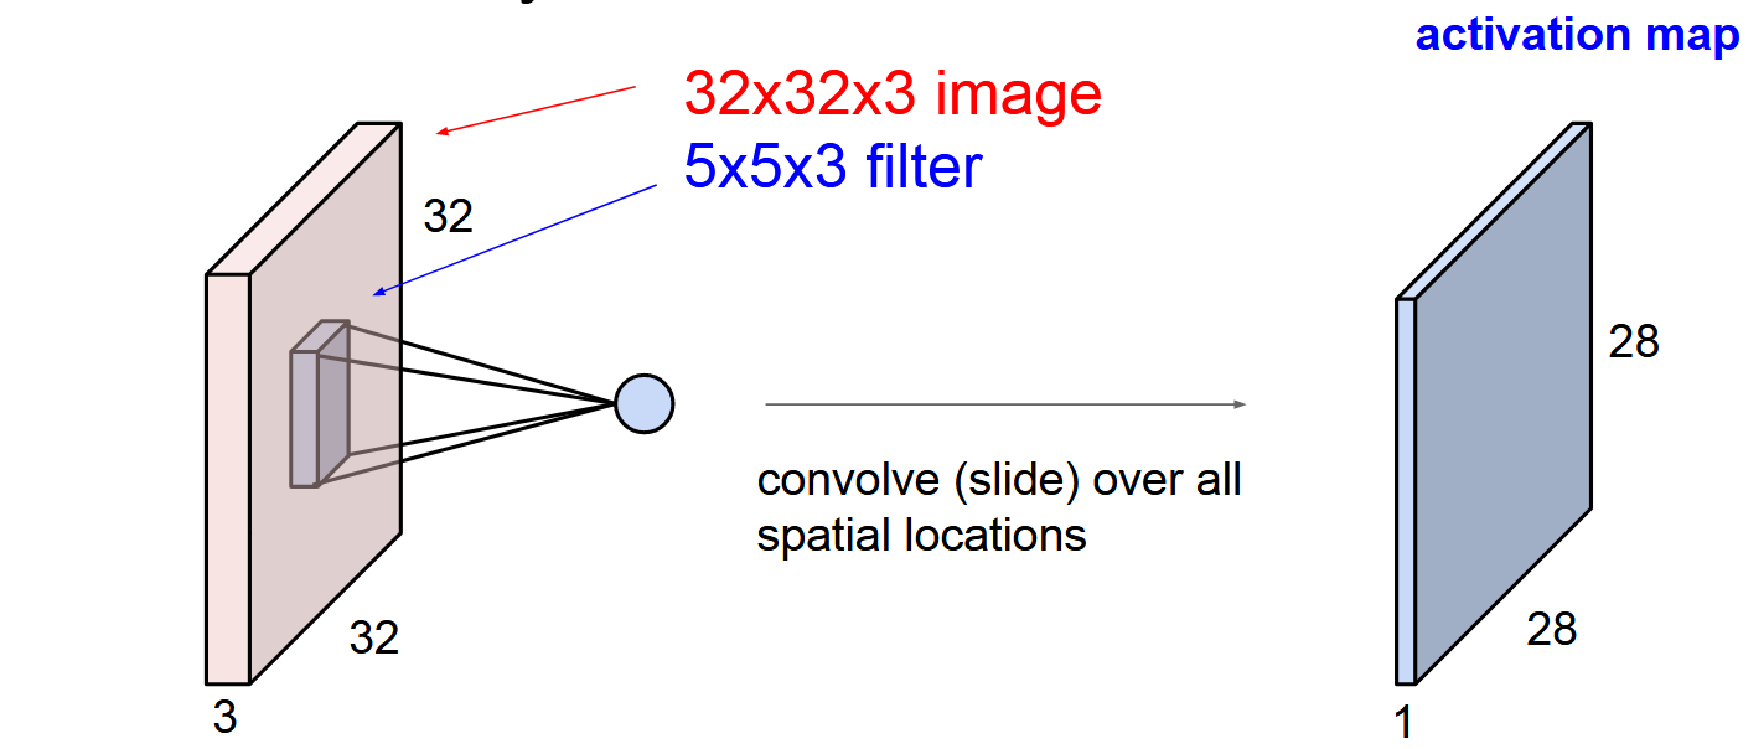
\includegraphics[scale=0.28]{L411.pdf}
\caption{Activation map}
\label{fig:L411}
\end{figure}
\end{minipage}\\\\
Surely more filters can be applied on an image , forming multiple \textbf{activation maps}, each shaped to look for \textbf{particular features or templates} in the picture \ref{fig:L412}.
\begin{figure}[h]
\centering
\captionsetup{justification=centering}
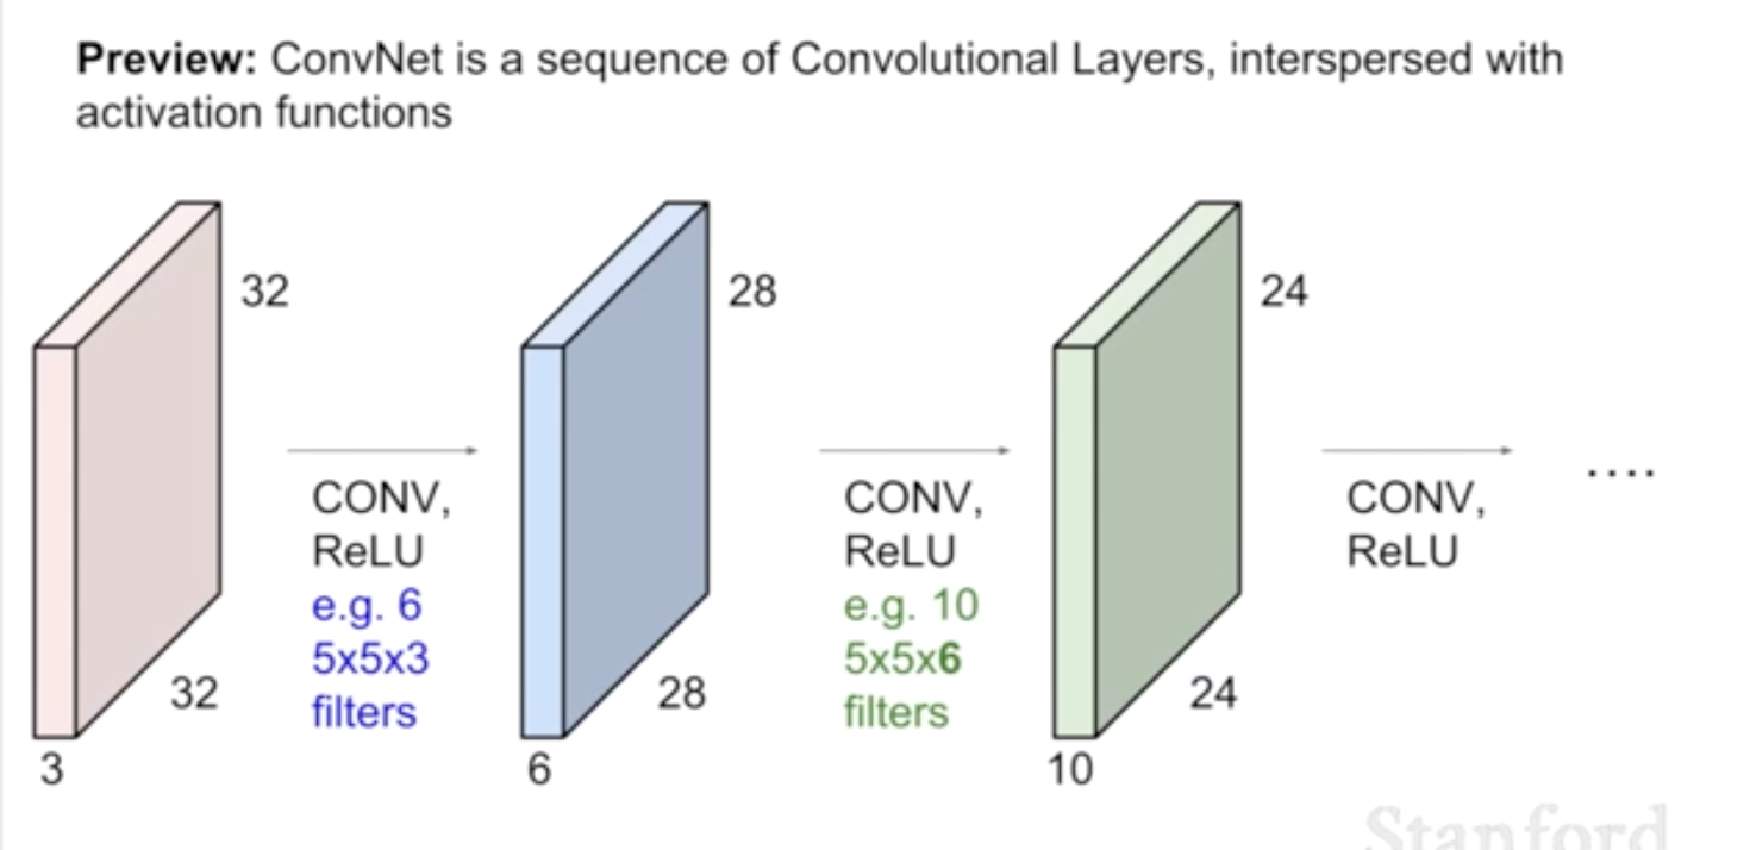
\includegraphics[width=0.7\linewidth]{L412.pdf}
\caption{ Sequence of convolutional layers}
\label{fig:L412}
\end{figure}
\clearpage
\textbf{Features recognised} become more and more complex along the convolution process \ref{fig:L413}.
\begin{figure}[h]
\centering
\captionsetup{justification=centering}
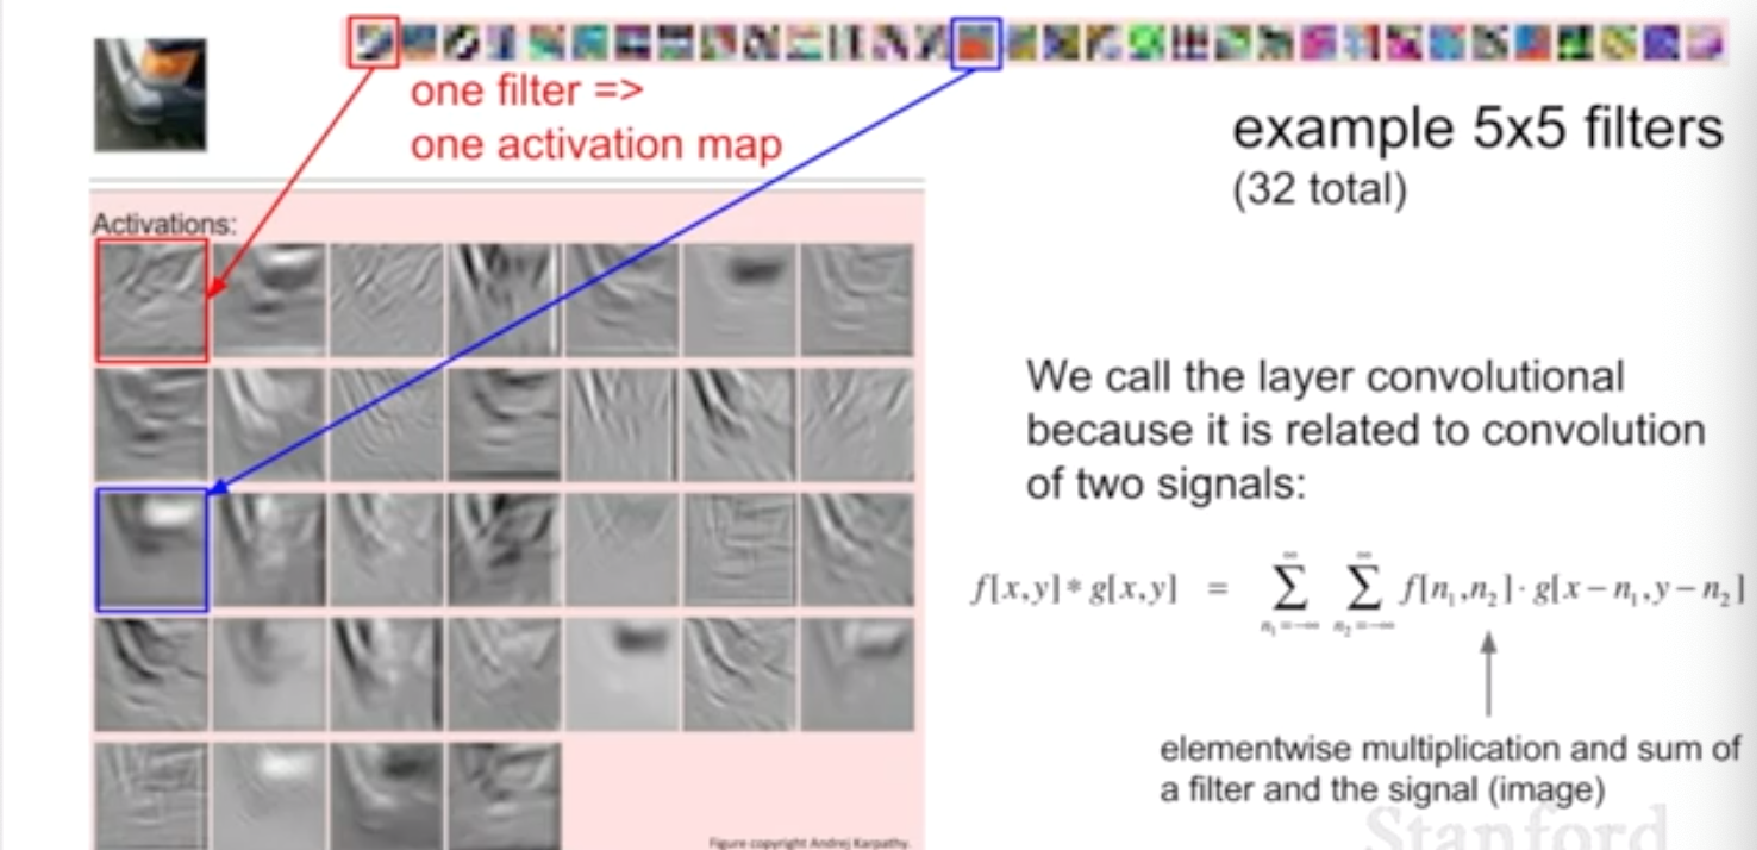
\includegraphics[width=0.8\linewidth]{L413.pdf}
\caption{ Complexity of features}
\label{fig:L413}
\end{figure}\\
To see how a \textbf{filter} works, consider 7x7 input and 3x3 filter : start from the upper left corner and multiply term by term. Then \textbf{slide} horizontally of one pixel at a time. Repeat the procedure also vertically. 
The output is an activation map with dimension $5x5$. The the pixel shift \textbf{or stride}, may vary with different problems. Make sure to be able to \textbf{cover the entire image}.
\begin{figure}[h]
\centering
\captionsetup{justification=centering}
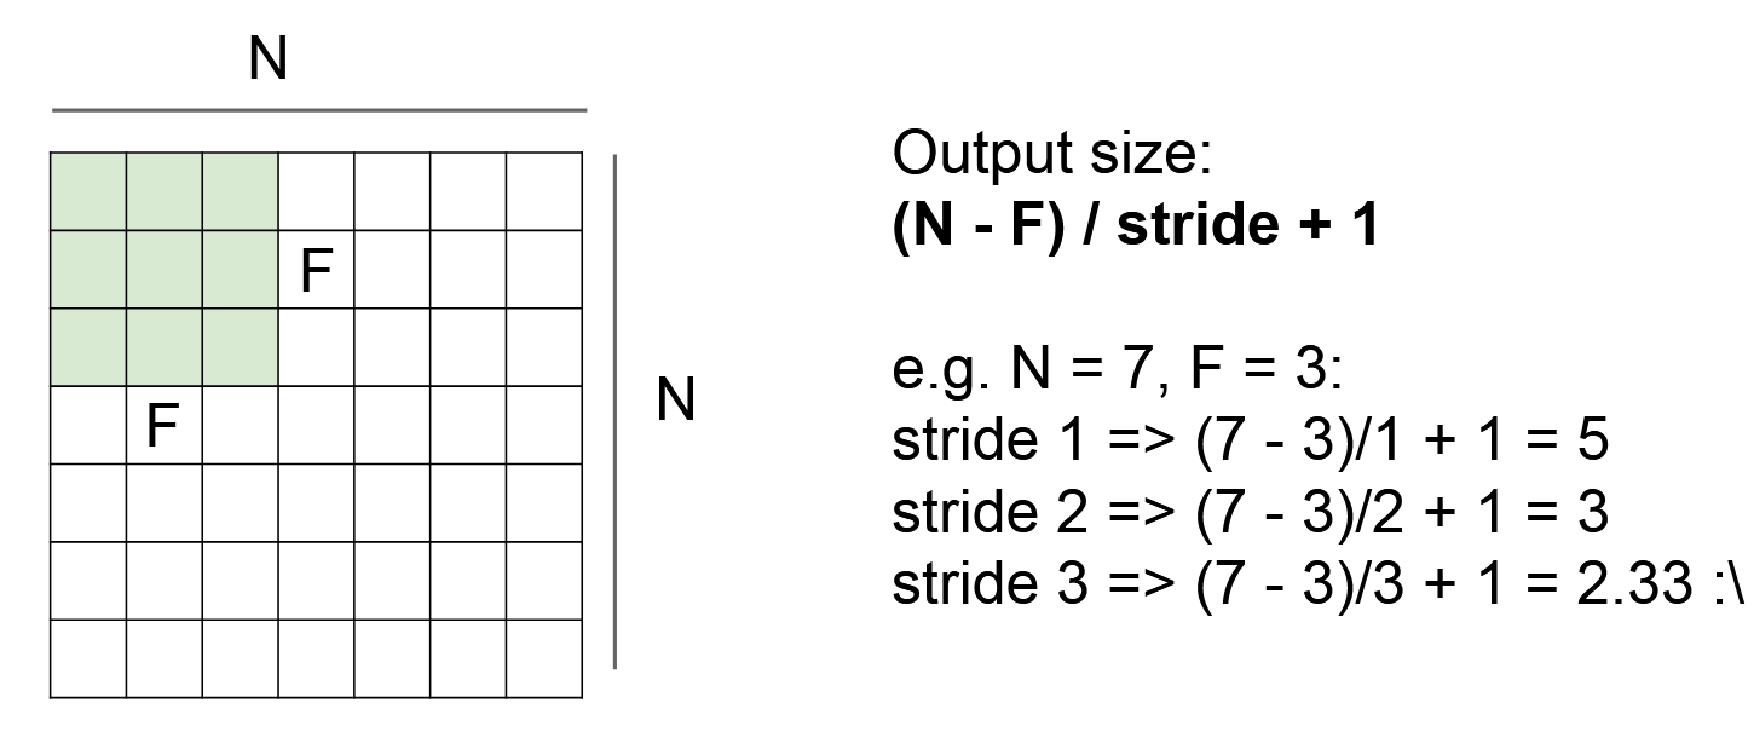
\includegraphics[width=0.7\linewidth]{L414.pdf}
\caption{ Sliding of the filter}
\label{fig:L414}
\end{figure}\\
A way to understand whether the \textbf{stride } is appropriate is proposed by the following formula:
\begin{equation}
    output_{size}= \frac{(N - F)}{stride} + 1 
\end{equation}{}
\textbf{ N} is the \textbf{image dimension} and \textbf{F} is the \textbf{filter dimension}. If the output size is not an integer, address the issue in  two ways:
\begin{enumerate}
    \item \textbf{Change the stride value}
    \item \textbf{Zero pad} to the border = hemming the matrix with zeros
\end{enumerate}{}
In general, it is common to see \textbf{CONV} layers with stride 1, filters of size $FxF$, and zero padding with $\frac{F-1}{2}$
\clearpage
The \textbf{activation maps} are \textbf{smaller} in dimension with respect to the input. A good practise is not to \textbf{shrink} too fast the dimension in one step.\\
\begin{minipage}{0.5\textwidth}
\begin{figure} [H]
\centering 
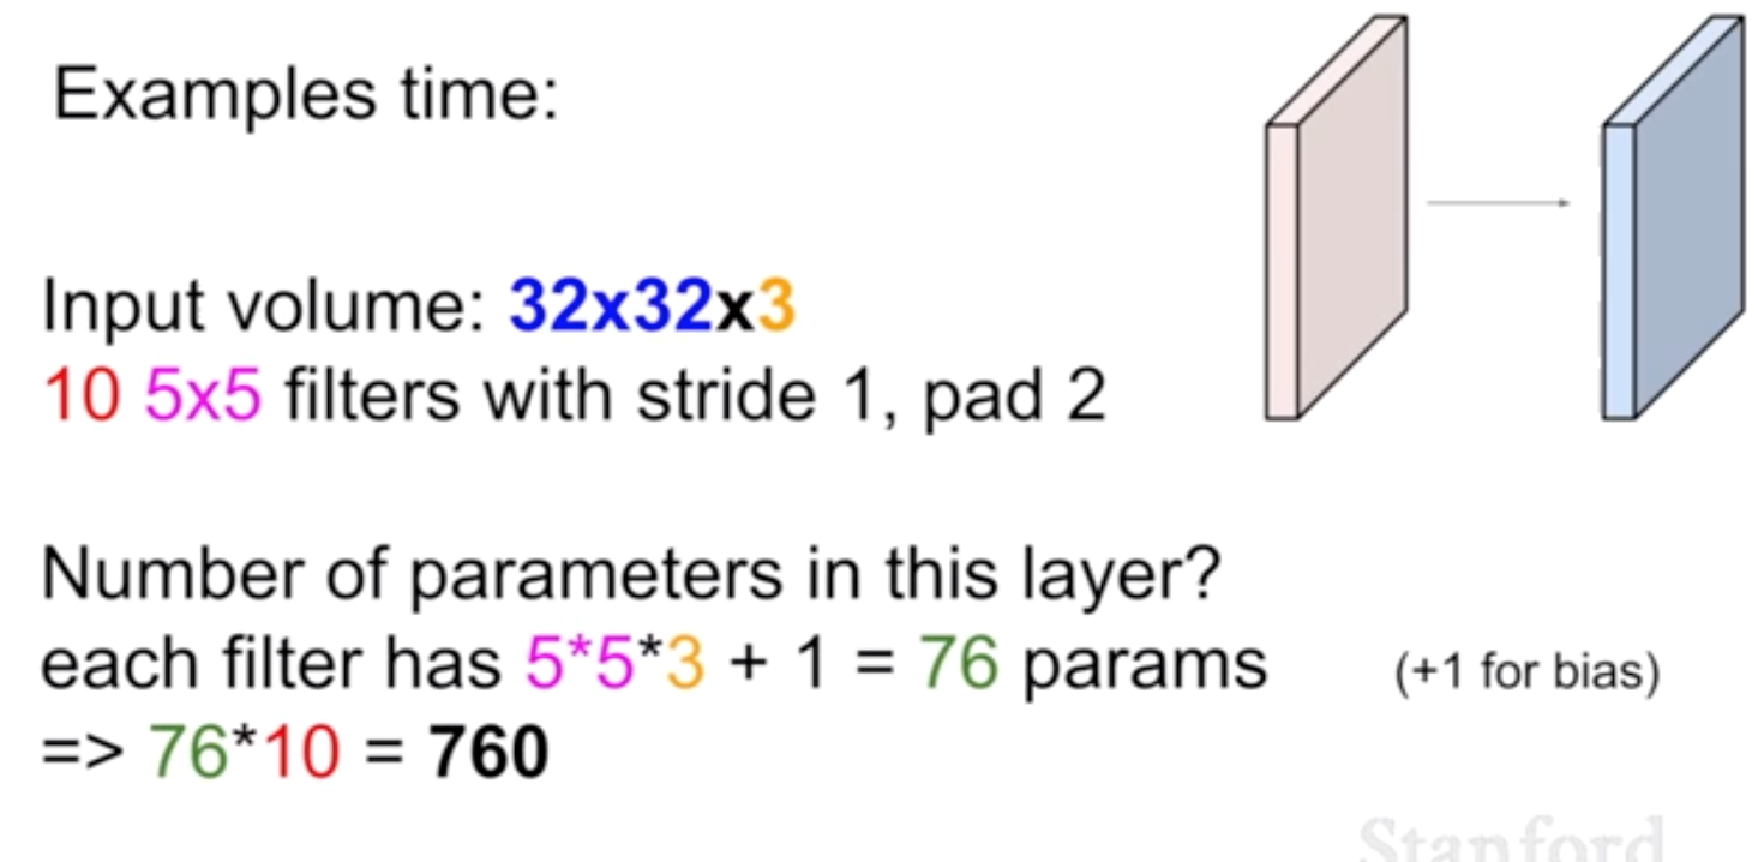
\includegraphics[scale=0.28]{L415.pdf}
\caption{ Example of activation map dimension}
\label{fig:L415}
\end{figure}
\end{minipage}
\begin{minipage}{0.5\textwidth}
\begin{figure} [H]
\centering 
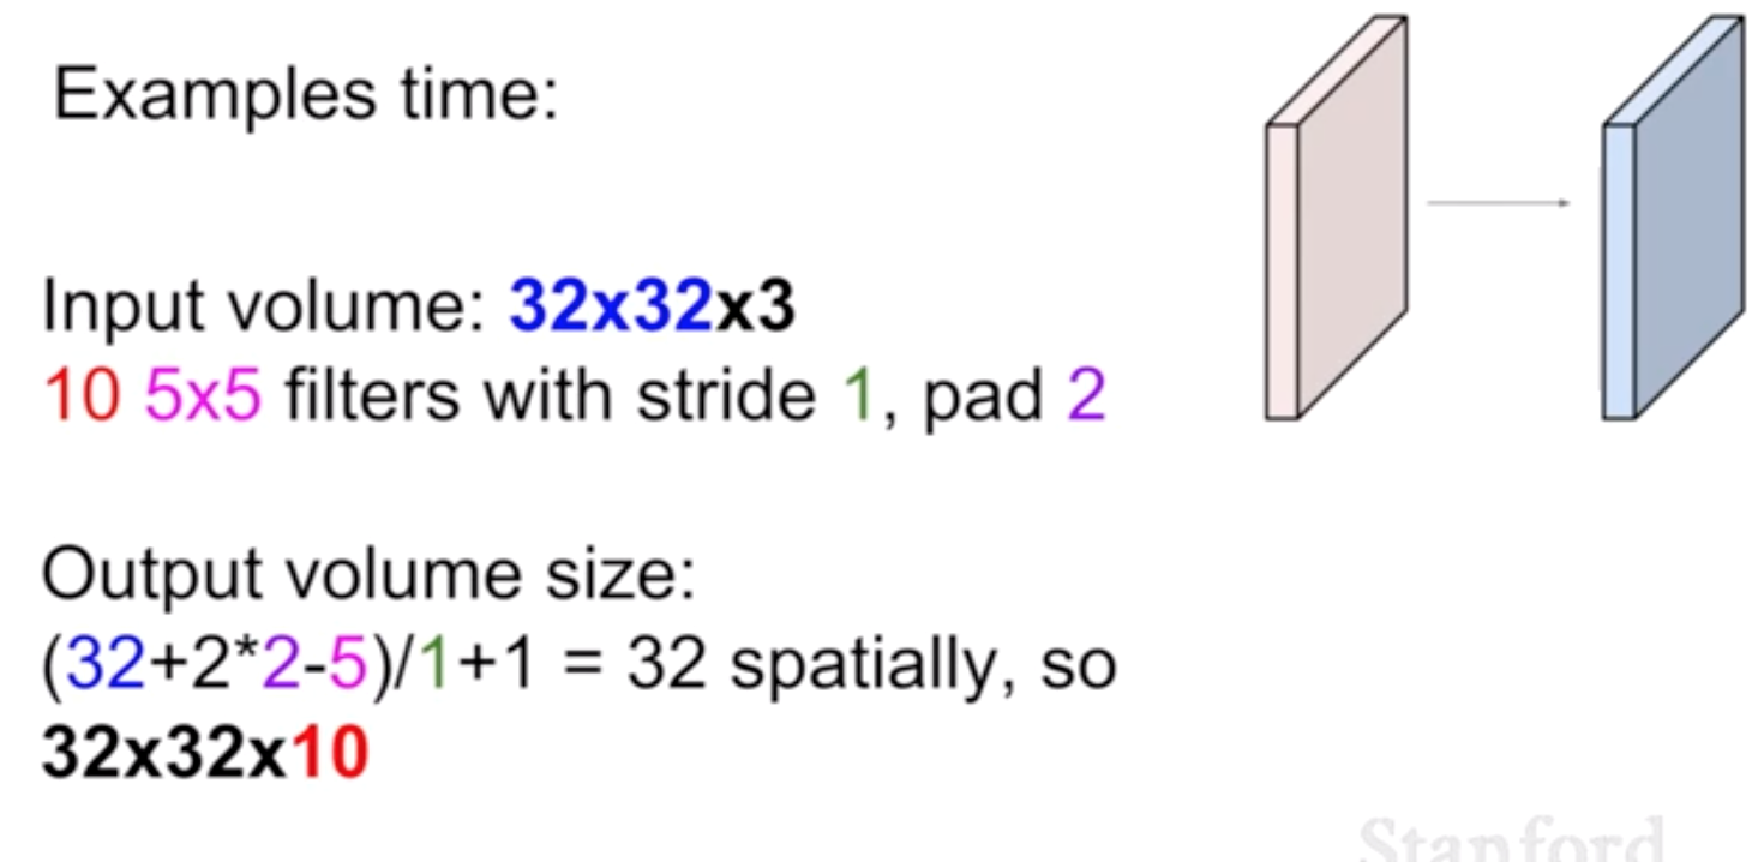
\includegraphics[scale=0.28]{L416.pdf}
\caption{Example of activation map dimension}
\label{fig:L416}
\end{figure}
\end{minipage}\\
\begin{figure}[h]
\centering
\captionsetup{justification=centering}
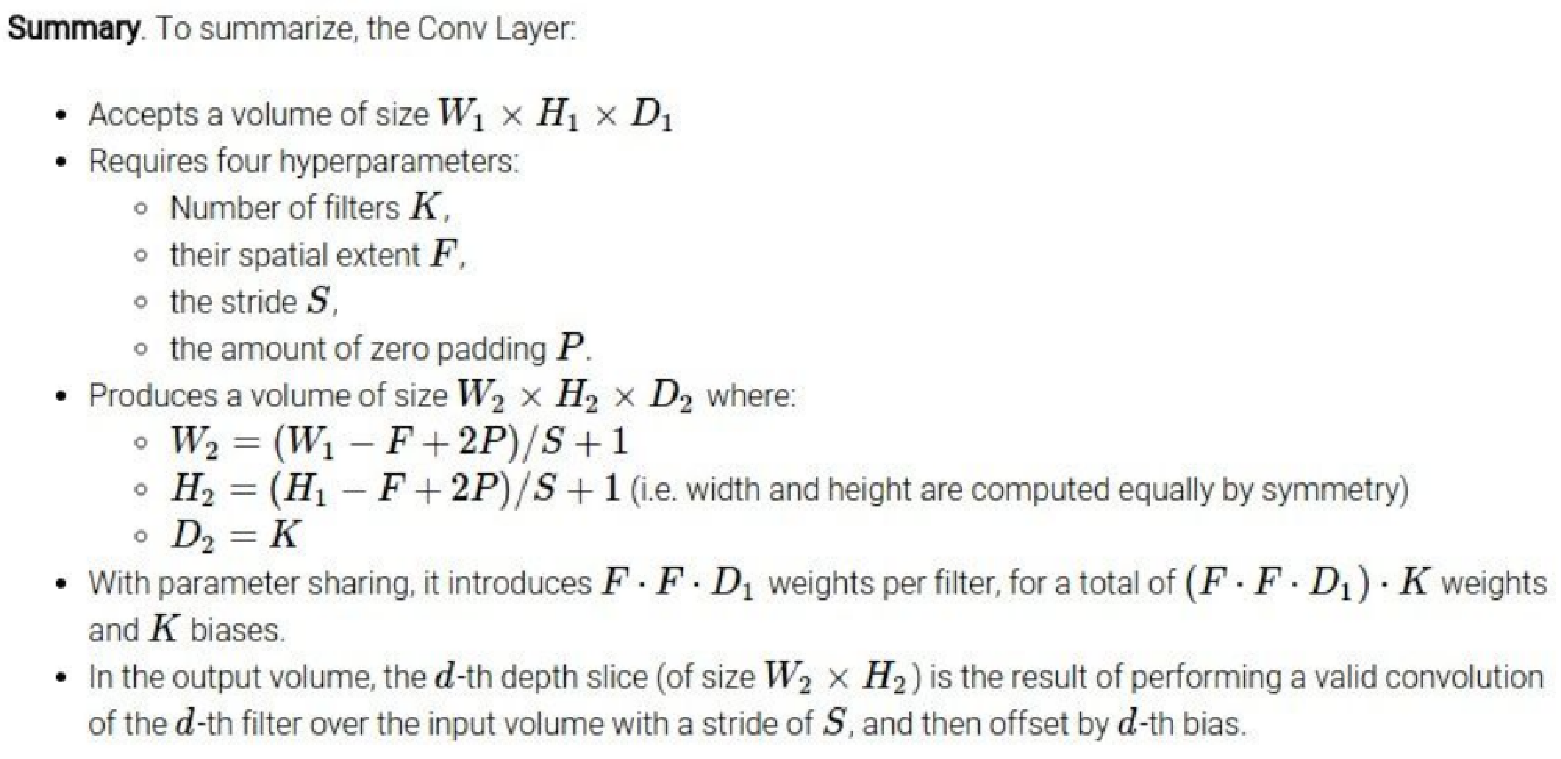
\includegraphics[width=0.9\linewidth]{L417.pdf}
\caption{ Summary on convolutional layers}
\label{fig:L417}
\end{figure}\\
In \textbf{CNNs} the neuron is only locally connected to the input \textit{(because a chunk of image  is convolved )}.
\clearpage
\paragraph{Pooling layer}
It makes the representation smaller and more manageable \textit{(downsampling spatially).}
It does not change in depth \textit{(color or else)} . It operates on each \textbf{activation map}.
\begin{figure}[h]
\centering
\captionsetup{justification=centering}
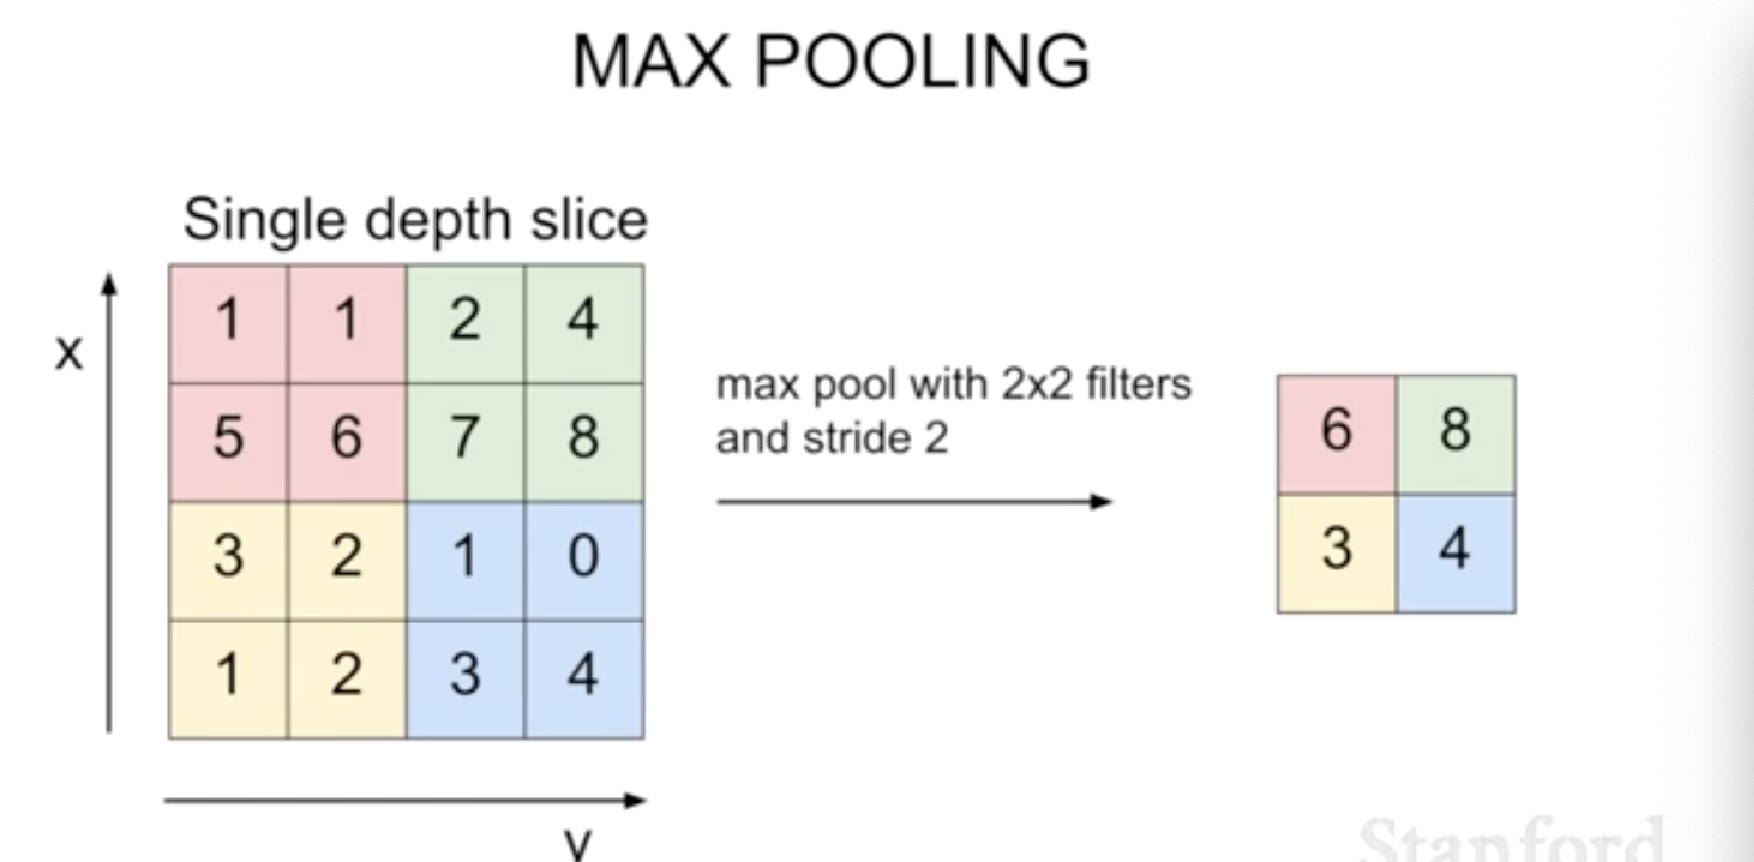
\includegraphics[width=0.7\linewidth]{L418.pdf}
\caption{ Max  pooling}
\label{fig:L418}
\end{figure}\\
\textbf{Max pooling} is better because it gives signal of the filter detecting some aspect of the image at its maximum. \textbf{Striding and pooling } are almost the same thing so striding can be used instead of pooling \textit{(even if it is not done).}
\begin{figure}[h]
\centering
\captionsetup{justification=centering}
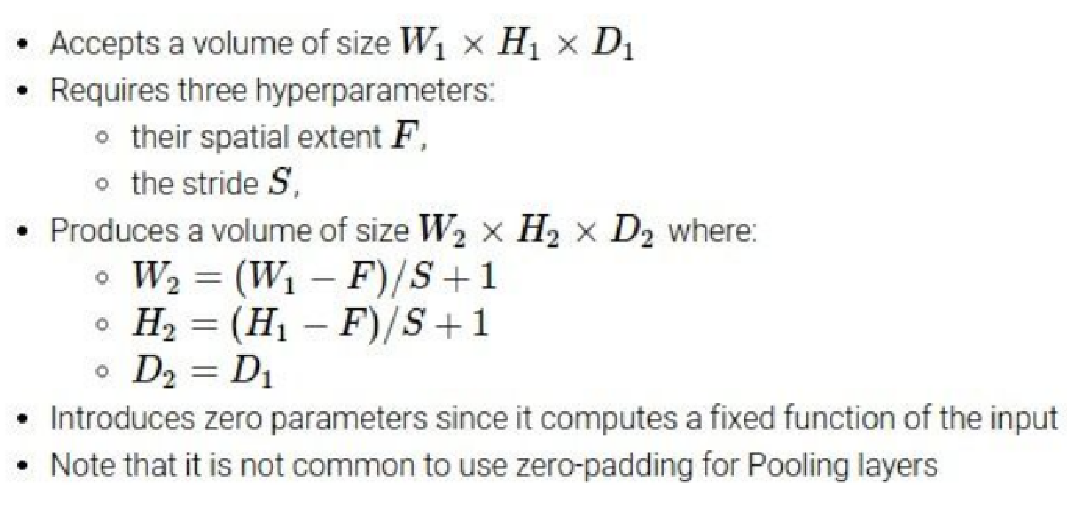
\includegraphics[width=0.75\linewidth]{L419.pdf}
\label{fig:L419}
\end{figure}\\
\textbf{Fully connected layers} contain neurons linked to the entire input volume, like in ordinary neural networks. At the last layer all the layers are aggregated  and taken them into account. How much pooling you have to do? Try and see 
\clearpage

\subsection{Lecture 6 | Training Neural Networks I}
\textbf{Youtube link:}\\
\url{https://www.youtube.com/watch?v=wEoyxE0GP2M&list=PL3FW7Lu3i5JvHM8ljYj-zLfQRF3EO8sYv&index=6}\\
\textbf{Slides:}\\
\url{http://cs231n.stanford.edu/slides/2017/cs231n_2017_lecture6.pdf}
\paragraph{Training neural networks}
The activations functions used in Neural networks are: \textbf{sigmoid, tanh, ReLU etc} \ref{fig:L316}\\\\
\begin{minipage}{0.5\textwidth}

\textbf{Sigmoid:}
\begin{enumerate}
    \item Squashes numbers to range [0,1]
    \item \textbf{Saturated neurons} set to \textbf{0 the gradients} :(
    \item Sigmoid outputs are \textbf{not zero-centered} :(
    \item $e^x$ is a bit compute expensive :(
\end{enumerate}{}

\textbf{tanh(x):}
\begin{enumerate}
    \item Squashes numbers to range [-1,1]
    \item \textbf{zero centered} (nice)
    \item still \textbf{kills gradients} when saturated :(
    
\end{enumerate}{}


\textbf{ELU}

\begin{enumerate}
    \item All benefits of\textbf{ ReLU}
    \item Closer to zero mean outputs 
    \item Negative saturation regime compared with Leaky ReLU adds some \textbf{robustness to noise }
     \item $e^x$ is a bit compute expensive :(
\end{enumerate}{}
\textbf{Leaky Relu}
\begin{enumerate}
    \item Does not saturate
    \item \textbf{Computationally efficient}
    \item \textbf{Converges much faster than sigmoid/tanh} in practice! (e.g. 6x)-will not die
\end{enumerate}{}
\end{minipage}
\begin{minipage}{0.5\textwidth}



\textbf{Relu}
\begin{enumerate}
    \item Does not saturate (in +region)
    \item \textbf{Very computationally efficient}
    \item \textbf{Converges much faster }than sigmoid/tanh in practice (e.g. 6x)-
    \item Actually more biologically plausible than sigmoid
    \item Not zero-centered output :(
    \item problem with negative values for the gradient :(
\end{enumerate}{}





\textbf{Maxout}
\begin{enumerate}
    \item Does not have the basic form of dot product -> nonlinearity
    \item G\textbf{eneralizes ReLU and Leaky ReLU }
    \item Linear Regime! \textbf{Does not saturate}! Does not die!
    \item doubles the number of parameters/neuron :(
\end{enumerate}{}
\end{minipage}\\
\paragraph{Data pre-processing}
\textbf{Zero centering} \textit{(subtract mean or channel (RGB) mean)} and normalizing \textit{(by a std deviation)}
Usually With images the normalization is not done .
\clearpage
\paragraph{Weight inizialization}
\begin{itemize}
    \item If all weights are set to 0: \textbf{all the neurons will do the same thing }(problem)
    \item first idea: \textbf{small random numbers, gaussian with zero mean and 0.01 std deviation}
  problems are encontered  with deep networks \textit{(std deviation collapses to 0)} => weight will get very \textbf{small gradients and not updating}.
  \item second idea: small random numbers, gaussian with zero mean and 1 std deviation. 
  By multiplying by high weights over and over neurons will be saturated, \textbf{ all gradients will be zero.}
\item \textbf{Xavier initialization},  scaling on the square root of number of the inputs. There is the assumption in the active region of data cloud.
Not working with \textbf{ReLU} \textit{(non linearity breaks)} . Try to divide the random distribution by the square root of half the number of the input \textit{(half neurons are dead)}.


\end{itemize}{}
\paragraph{Batch normalization}
\textbf{Batch normalization} is a way to boost the speed, performance, and stability of artificial neural networks. It is used to \textbf{normalize} the input layer by \textbf{adjusting and scaling} the activations. Consider a batch of activations at some layer. To make each dimension \textbf{unit gaussian}, apply:
\begin{equation}
    \hat{\mathbf{x}}^k=\frac{\mathbf{x}^k -E(\mathbf{x}^k)}{\sqrt{Var(\mathbf{x}^k})}
\end{equation}{}
The way forward is:
\begin{enumerate}
    \item compute the \textbf{empirical mean and variance} independently for each dimension
    \item normalize
\end{enumerate}{}
Usually inserted after \textbf{Fully Connected or Convolutional layers, and before nonlinearity.}\\
Positive aspects about batch normalization:
\begin{enumerate}
    \item \textbf{Improves gradient} flow through the network
    \item Allows \textbf{higher learning rates}
    \item Reduces the strong dependence on initialization
    \item Acts as a form of \textbf{regularization} in a funny way, and slightly reduces the need for dropout, maybe
\end{enumerate}{}
Here are shown the different steps to perform a normalization:\\\\
\begin{minipage}{0.5\textwidth}
\textbf{Mini-batch mean}
\begin{equation}
    \mu_b=\frac{1}{m}\sum_{i=1}^{m}x_i
\end{equation}{}

\textbf{Mini-batch variance}
\begin{equation}
    \sigma_b=\frac{1}{m}\sum_{i=1}^{m}(x_i-\mu_b)^2
\end{equation}{}

\end{minipage}
\begin{minipage}{0.5\textwidth}
\textbf{Normalize}
\begin{equation}
     \hat{x}_i=\frac{x_i -E(\mathbf{x})}{\sqrt{Var(\mathbf{x}^k})}
\end{equation}{}
\textbf{Scale and shift}
\begin{equation}
    y_i= \gamma x_i+\beta=\mathbf{BN}(x_i)_{\gamma,\beta}
\end{equation}{}
\end{minipage}\\
Why learning \textbf{gamma and beta}? Because it  gives flexibility, sometimes it is not useful to take the same normalization as the other parts, so the original mapping is recovered and another normalization is adopted  \textit{(or scaled using other parameters learned)}.\textbf{Mean and std deviation} used at \textbf{test }time are the same used in the inputs scaling at \textbf{training} time.
\paragraph{Babysitting the learning process}
\begin{enumerate}
    \item Pre-process the data
    \item Choose the architecture
    \item Double check the loss
\end{enumerate}{}
\begin{figure}[h]
\centering
\captionsetup{justification=centering}
\includegraphics[width=0.9\linewidth]{L510.pdf}
\caption{ Loss check}
\label{fig:L510}
\end{figure}

\textbf{Sanity checks} = Firstly determine the loss without the regularization. Then switch on regularization and notice if the loss goes up \textit{(which would be normal)}.\\


At the beginning of the training, start up with a \textbf{small amount of data}, because it \textbf{over fits well } and the loss gives good results, reaching a value close to 0, after few epochs.

\paragraph{Learning rate and hyperparameters}
After the \textbf{ sanity checks } the real training can begin, starting from a small value of the regularization term \textit{(e.g 0.000001)}. Subsequently figure out which is the proper value for the \textbf{learning rate}.If the loss is barely changing \textit{(not going down)} probably the learning rate is\textbf{ too low.} Even if the Loss does not change, a \textbf{jump } in the \textbf{accuracy} is expected: the probabilities are slightly changed and the problem is moving toward the right solution. On the other hand a high value of learning rate $\mathbf{10^{6}}$, the loss will return a \textbf{nan} value, because it is exploding.
As a rule of thumb is to select the learning rate for the cross validation between $\mathbf{10^{-3}}$ and $\mathbf{10^{-5}}$.
\paragraph{Hyparameter optimization}
For each hyperparameter the \textbf{cross validation} is done: training on your training set, and then evaluating on the validation set. In this way it is possible to establish how good a hyperparameter is.\\
Step:
\begin{enumerate}
    \item \textbf{First stage:} only a few epochs to get rough idea of how a parameter works
    \item \textbf{Second stage}: longer running time, finer search... \textit{(repeat as necessary)}
\end{enumerate}{}
Tip for detecting explosions in the solver: If the \textbf{cost} is $ > 3 \cdot original \ cost$, it breaks out early.
\begin{figure}[h]
\centering
\captionsetup{justification=centering}
\includegraphics[width=0.9\linewidth]{L511.pdf}
\caption{ Hyperparameters optimization example}
\label{fig:L511}
\end{figure}
\begin{figure}[h]
\centering
\captionsetup{justification=centering}
\includegraphics[width=0.9\linewidth]{L512.pdf}
\caption{ Hyperparameters optimization example}
\label{fig:L512}
\end{figure}\\
It is helpful to have a \textbf{random layout} between an important parameter vs the unimportant one: more chances to get greater results
\clearpage
\begin{minipage}{0.5\textwidth}
\begin{figure} [H]
\centering 
\includegraphics[scale=0.55]{L513.pdf}
\caption{ Grid layout vs random layout}
\label{fig:L513}
\end{figure}

\begin{figure} [H]
\centering 
\includegraphics[scale=0.58]{L514.pdf}
\caption{ Loss vs hyperparametrs}
\label{fig:L514}
\end{figure}



\end{minipage}
\begin{minipage}{0.5\textwidth}
\begin{figure} [H]
\centering 
\includegraphics[scale=0.52]{L515.pdf}
\caption{ Bad initialization}
\label{fig:L515}
\end{figure}

\begin{figure} [H]
\centering 
\includegraphics[scale=0.58]{L516.pdf}
\caption{ Accuracy}
\label{fig:L516}
\end{figure}

\end{minipage}\\\\
In \ref{fig:L516} a \textbf{big gap} between the curves is a problem of overfitting => increase the regularization. No gap means increase the model capacity?
\clearpage
\subsection{Lecture 7 | Training Neural Networks II}
\textbf{Youtube link:}\\
\url{https://www.youtube.com/watch?v=_JB0AO7QxSA&list=PL3FW7Lu3i5JvHM8ljYj-zLfQRF3EO8sYv&index=7}\\
\textbf{Slides:}\\
\url{http://cs231n.stanford.edu/slides/2017/cs231n_2017_lecture7.pdf}
\paragraph{Optimization}
The loss function at each step tells how good  or bad the weights prediction is. In order to  update the weights an example could be the \textbf{Stocastic gradient descent SGD}:
\begin{equation}
    \mathbf{W_{new}}=\mathbf{W_{old}}-l_{rate}\cdot \nabla_W L(\mathbf{W_{old}})
\end{equation}{}
What if loss changes quickly in one direction and slowly in another? What does gradient descent do? Loss function has high \textbf{condition number}: ratio of largest to smallest singular value of the Hessian matrix is large. \\
\textbf{SGD drawbacks :}
\begin{enumerate}
    \item  Very slow progress along\textbf{ shallow dimension, jitter along steep direction.}
    \item Local minima will get \textbf{SGD} stuck because the gradient will be 0 \textit{(no progress)}.
With saddle points same thing

\end{enumerate}{}
\begin{minipage}{0.5\textwidth}
\textbf{SGD}\\
\begin{equation}
    x_{t+1}=x_t-\alpha \nabla f(x_t)
\end{equation}{}
the relative code:\\
\begin{figure} [H]
\centering 
\includegraphics[scale=0.58]{L610.pdf}
\caption{ \textbf{SGD}}
\label{fig:L610}
\end{figure}


\end{minipage}
\begin{minipage}{0.5\textwidth}

\textbf{SGD + momentum}
\begin{equation}
\begin{cases}
v_{t+1}=\rho v_t+\nabla f(x_t) \\
    x_{t+1}=x_t-\alpha v_{t+1}
    \end{cases}{}
\end{equation}{}

the relative code:
\begin{figure} [H]
\centering 
\includegraphics[scale=0.58]{L611.pdf}
\caption{ \textbf{SGD} + momentum}
\label{fig:L611}
\end{figure}


\end{minipage}\\\\
\textbf{SGD + momentum}
\begin{enumerate}
    \item  Build up velocity as a running mean of gradient
    \item $\rho $ gives friction; typically $\rho$=0.9 or 0.99
    \item Initial velocity = 0 usually
\end{enumerate}
\clearpage
\begin{minipage}{0.5\textwidth}

\begin{figure} [H]
\centering 
\includegraphics[scale=0.46]{L612.pdf}
\caption{ \textbf{SGD} + momentum optimization}
\label{fig:L612}
\end{figure}
\end{minipage}
\begin{minipage}{0.5\textwidth}
\begin{figure} [H]
\centering 
\includegraphics[scale=0.58]{L613.pdf}
\caption{ \textbf{SGD} + momentum vectors}
\label{fig:L613}
\end{figure}
\end{minipage}\\\\
\paragraph{Nesterov momentum}
\begin{equation}
\begin{cases}{}
    v_{t+1}=\rho v_t+\nabla f(x_t+\rho v_t)\\
    x_{t+1}= x_t+\alpha v_{t+1}
    \end{cases}{}
\end{equation}{}
With the following change of variables :
\begin{equation}
    \hat{x}_{t}= x_t+\rho v_t
\end{equation}{}
The formulation of the method becomes


\begin{minipage}{0.5\textwidth}
\begin{equation}
\begin{cases}
v_{t+1}=\rho v_t+\nabla f(\hat{x}_t) \\
    \hat{x}_{t+1}=\hat{x}_t+v_{t+1} -\alpha v_{t+1} \rho (v_{t+1}-v_t)
    \end{cases}{}
\end{equation}{}
\end{minipage}
\begin{minipage}{0.5\textwidth}
\begin{figure} [H]
\centering 
\includegraphics[scale=0.46]{L614.pdf}
\caption{ Nesterov momentum code}
\label{fig:L614}
\end{figure}
\end{minipage}\\\\


With \textbf{nesterov momentum },  the first step is done  according to the  velocity then go back to the original point and combine the gradient with velocity direction.
Usually \textbf{nesterov momentum } and \textbf{SGD +momentum } overshoot the minimum, due to a building up velocity and then they correct themselves going back to the minimum.\\
\paragraph{Adagrad}
During the course of optimization, keep a running estimate or a running sum of all the squared gradients seen during training . Instead of having a velocity term there is a \textbf{Grad squared} term.
The weights are updated in the following way:

\begin{minipage}{0.5\textwidth}
\begin{equation}
\begin{cases}
\nabla_{sq_{new}} = \nabla_{sq_{old}} + \nabla_W L(\mathbf{W_{old}})^T\cdot \nabla_W L(\mathbf{W_{old}}) \\\\
\mathbf{W_{new}} = \mathbf{W_{old}}+l_{rate}
 \cfrac{\nabla_W L(\mathbf{W_{old}})}{\sqrt{\nabla_{sq_{new}}}+10^{-7}}
 \end{cases}
\end{equation}{}
\end{minipage}
\begin{minipage}{0.5\textwidth}
\begin{figure} [H]
\centering 
\includegraphics[scale=0.60]{L615.pdf}
\caption{ Adagrad code}
\label{fig:L615}
\end{figure}
\end{minipage}\\\\
With this scaling in \textbf{Adagrad } the step  becomes smaller and smaller overtime and slows down in the wiggling dimension. In the convex case this is a good feature to have : it is better to slow down close to the minimum. Issues come up with \textbf{non convex problems} for example  with saddle points where the method may be get stuck, without making any progress. $10^{-7}$ is in the denominator to avoid $0$ values at the denominator
\paragraph{RMSprop}
\textbf{RMSprop} is based on the \textbf{Adagrad } a procedure.With the introduction of a decay rate it is able to avoid being stuck in saddle point as \textbf{Adagrad } does. 
\begin{figure}[h]
\centering
\captionsetup{justification=centering}
\includegraphics[width=0.9\linewidth]{L616.pdf}
\caption{ \textbf{RMSprop} code}
\label{fig:L616}
\end{figure}

\paragraph{Adam}
\begin{figure}[h]
\centering
\captionsetup{justification=centering}
\includegraphics[width=0.9\linewidth]{L617.pdf}
\caption{ \textbf{Adam} full form}
\label{fig:L617}
\end{figure}
2 moments with a \textbf{bias} in order not to have a too large step at the beginning.
All the methods have a learning rate, changing during the training:
large at the beginning then \textbf{decreasing}
\textit{(step decaying or decaying by a law)}\\\\
\begin{minipage}{0.5\textwidth}
\begin{equation}
    \alpha = \alpha_0 e^{-kt}
\end{equation}{}
\end{minipage}
\begin{minipage}{0.5\textwidth}
\begin{equation}
    \alpha=\frac{\alpha_0}{1+kt}
\end{equation}{}
\end{minipage}

\paragraph{second order Optmization}
\begin{minipage}{0.5\textwidth}
\begin{figure} [H]
\centering 
\includegraphics[scale=0.54]{L618.pdf}
\caption{ First order optimization}
\label{fig:L618}
\end{figure}
\end{minipage}
\begin{minipage}{0.5\textwidth}
\begin{figure} [H]
\centering 
\includegraphics[scale=0.54]{L619.pdf}
\caption{ Second order optimization}
\label{fig:L619}
\end{figure}
\end{minipage}\\\\
Given the Taylor expansion stopped at the $2^{nd}$ order of a certain function
\begin{equation}
    J(\boldsymbol{\theta}) \approx     J(\boldsymbol{\theta_0}) +(\boldsymbol{\theta}-\boldsymbol{\theta_0})^T\nabla_{\theta} J(\boldsymbol{\theta_0})+\frac{1}{2}(\boldsymbol{\theta}-\boldsymbol{\theta_0})^T\mathbf{H}(\boldsymbol{\theta}-\boldsymbol{\theta_0})
\end{equation}{}
It can be found the position referred to the minimum of the quadratic function as:
\begin{equation}
 \boldsymbol{\theta^*}= \boldsymbol{\theta_0}- \mathbf{H}^{-1} \nabla_{\theta} J(\boldsymbol{\theta_0}) 
\end{equation}{}
positive aspects of $2^{nd}$ order optimization:
\begin{enumerate}
    \item No hyperparameters!
    \item No learning rate!
\end{enumerate}{}
drawbacks
\begin{enumerate}
    \item Hessian has $O(N^2)$ element,Inverting takes $O(N^3)$
    \item N = (Tens or Hundreds of) Millions
\end{enumerate}{}
\textbf{Quasi-Newton methods (BGFS most popular)}:instead of inverting the Hessian $O(N^3)$ , approximate inverse Hessian with rank 1 updates over time ($O(N^2)$  each).
\textbf{L-BFGS (Limited memory BFGS)}: Does not form/store the full inverse Hessian.\\
\textbf{L-BFGS (Limited memory BFGS)}:
\begin{enumerate}
    \item \textbf{Usually works very well in full batch, deterministic mode} i.e. if you have a single, deterministic f(x) then L-BFGS will probably work very nicely
    \item \textbf{Does not transfer very well to mini-batch setting}. Gives bad results. Adapting L-BFGS to large-scale, stochastic setting is an active area of research
\end{enumerate}{}

To sum up \textbf{Adam }is a good default choice in most cases. If you can afford to do full batch updates then try out \textbf{ L-BFGS} \textit{ (and do not forget to disable all sources of noise)}.
\clearpage
\paragraph{beyond the training error}
Practically the training error is only marginally important in a network. What really matters is \textbf{ the performance on unseen data}.
Model ensembles to reduce the difference of performance between training and testing data
Train multiple independent models, and average their results.

\begin{figure}[h]
\centering
\captionsetup{justification=centering}
\includegraphics[width=1\linewidth]{L620.pdf}
\caption{ Model Ensembles: Tips and Tricks}
\label{fig:L620}
\end{figure}
\begin{figure}[h]
\centering
\captionsetup{justification=centering}
\includegraphics[width=0.7\linewidth]{L621.pdf}
\caption{ Polyak averaging}
\label{fig:L621}
\end{figure}
How to improve performance of a single model: regularization=> add term to the loss \textit{(not useful for neural networks)}
\begin{equation}
    L= \frac{1}{N} \sum_{i=1}^{N} \sum_{j\neq y_i} max(0,f(x_i,\mathbf{W})_j f(x_i,\mathbf{W})_{y_i} +1) +\lambda R(\mathbf{W})
\end{equation}{}
$R(\mathbf{W})$ can be the $L_1$ or $L_2$ norm or a combination of both \ref{norm}.
\clearpage
\paragraph{Dropout}
\textbf{Dropout} is used: In each forward pass, randomly set some neurons to 0. Probability of dropping is a hyperparameter; 0.5 is common.Widely used  in \textbf{FC} layers, less common in convolutional layers.

\begin{figure}[h]
\centering
\captionsetup{justification=centering}
\includegraphics[width=0.8\linewidth]{L622.pdf}
\caption{ Dropout}
\label{fig:L622}
\end{figure}
\textbf{Dropout} Forces the network to have a redundant representation; Prevents co-adaptation of features.\textbf{Dropout} makes our output random!.
\begin{equation}
    y = f_W(x,z)
\end{equation}{}
$z$ is the random mask.Want to average out the randomness at test-time
\begin{equation}
    f(x) =E_z[f(x,z)]=\int p(z)f(x,z)dz
\end{equation}{}
\begin{figure}[h]
\centering
\captionsetup{justification=centering}
\includegraphics[width=0.8\linewidth]{L623.pdf}
\caption{ Dropout example}
\label{fig:L623}
\end{figure}\\\\
\textbf{Training}: Add some kind of randomness.\\
\textbf{Testing}: Average out randomness (sometimes approximate)
\clearpage
\begin{figure}[h]
\centering
\captionsetup{justification=centering}
\includegraphics[width=1\linewidth]{L624.pdf}
\caption{ Dropout example}
\label{fig:L624}
\end{figure}

Also inverted dropout is common.
\paragraph{Data augmentation}
\textbf{Modify randomly the image} during training and average these modifications out during testing
\begin{multicols}{3}
\begin{enumerate}
    \item translation
    \item rotation
    \item stretching
    \item shearing
    \item distortion
    \item color offset
\end{enumerate}{}

\end{multicols}{}
\begin{figure}[h]
\centering
\captionsetup{justification=centering}
\includegraphics[width=0.7\linewidth]{L625.pdf}
\caption{ Regularization}
\label{fig:L625}
\end{figure}
\clearpage
\paragraph{Transfer learning}
To train a \textbf{CNN} it is not needed a large amount of data to train the model.
\begin{figure}[h]
\centering
\captionsetup{justification=centering}
\includegraphics[width=0.7\linewidth]{L626.pdf}
\caption{ Transfer learning with \textbf{CNNs}}
\label{fig:L626}
\end{figure}

\begin{figure}[h]
\centering
\captionsetup{justification=centering}
\includegraphics[width=0.7\linewidth]{L627.pdf}
\caption{ Transfer learning with \textbf{CNNs}}
\label{fig:L627}
\end{figure}

\clearpage
\subsection{Lecture 8 | Deep Learning Software}
\textbf{Youtube link:}\\
\url{https://www.youtube.com/watch?v=6SlgtELqOWc&list=PL3FW7Lu3i5JvHM8ljYj-zLfQRF3EO8sYv&index=8}\\
\textbf{Slides:}\\
\url{http://cs231n.stanford.edu/slides/2017/cs231n_2017_lecture8.pdf}
\paragraph{Tensorflow}

\begin{figure}[h]
\centering
\captionsetup{justification=centering}
\includegraphics[width=0.9\linewidth]{L710.pdf}
\caption{ Tensorflow code example}
\label{fig:L710}
\end{figure}

\begin{figure}[h]
\centering
\captionsetup{justification=centering}
\includegraphics[width=0.9\linewidth]{L711.pdf}
\caption{ Tensorflow code example}
\label{fig:L711}
\end{figure}
\clearpage

\begin{figure}[h]
\centering
\captionsetup{justification=centering}
\includegraphics[width=0.9\linewidth]{L712.pdf}
\caption{ Tensorflow code example}
\label{fig:L712}
\end{figure}
\paragraph{Keras}
\textbf{Keras } is a layer on top of \textbf{TensorFlow}, makes common things easy to do(Also supports Theano backend)
\begin{figure}[h]
\centering
\captionsetup{justification=centering}
\includegraphics[width=0.9\linewidth]{L713.pdf}
\caption{ Keras code example}
\label{fig:L713}
\end{figure}
\clearpage
\paragraph{Pytorch}
\begin{itemize}
    \item \textbf{Tensor:} Imperative ndarray, but runs on GPU
    \item \textbf{Variable:} Node in a computational graph; stores data and gradient
    \item \textbf{Module}: A neural network layer; may store state or learnable weights
\end{itemize}{}
\begin{figure}[h]
\centering
\captionsetup{justification=centering}
\includegraphics[width=0.9\linewidth]{L714.pdf}
\caption{ Pytorch code example}
\label{fig:L714}
\end{figure}

\begin{figure}[h]
\centering
\captionsetup{justification=centering}
\includegraphics[width=1\linewidth]{L715.pdf}
\caption{ Pytorch code example}
\label{fig:L715}
\end{figure}

\begin{figure}[h]
\centering
\captionsetup{justification=centering}
\includegraphics[width=1\linewidth]{L716.pdf}
\caption{ Pytorch code example}
\label{fig:L716}
\end{figure}

\begin{figure}[h]
\centering
\captionsetup{justification=centering}
\includegraphics[width=1\linewidth]{L717.pdf}
\caption{ Pytorch code example}
\label{fig:L717}
\end{figure}

\begin{figure}[h]
\centering
\captionsetup{justification=centering}
\includegraphics[width=1\linewidth]{L718.pdf}
\caption{ Pytorch code example}
\label{fig:L718}
\end{figure}

\clearpage
\paragraph{Static vs dynamic graph}
\begin{figure}[h]
\centering
\captionsetup{justification=centering}
\includegraphics[width=1\linewidth]{L719.pdf}
\caption{ static vs dynamic graph}
\label{fig:L719}
\end{figure}
\begin{figure}[h]
\centering
\captionsetup{justification=centering}
\includegraphics[width=1\linewidth]{L720.pdf}
\caption{ static vs dynamic graph}
\label{fig:L720}
\end{figure}
Static vs dynamic graph:
\begin{itemize}
    \item \textbf{Static:} Once graph is built, can serialize it and run it without the code that built the graph!
    \item \textbf{Dynamic:} Graph building and execution are intertwined, so always need to keep code around
\end{itemize}{}

\textbf{Dynamic Graph Applications} : Recurrent networks,Recursive networks,Modular Networks


\clearpage

\subsection{Lecture 9 | CNN Architectures}
\textbf{Youtube link:}\\
\url{https://www.youtube.com/watch?v=DAOcjicFr1Y&list=PL3FW7Lu3i5JvHM8ljYj-zLfQRF3EO8sYv&index=9}\\
\textbf{Slides:}\\
\url{http://cs231n.stanford.edu/slides/2017/cs231n_2017_lecture9.pdf}

\paragraph{CNNs}

\begin{figure}[h]
\centering
\captionsetup{justification=centering}
\includegraphics[width=0.82\linewidth]{L810.pdf}
\caption{ Alexa net}
\label{fig:L810}
\end{figure}
%\paragraph{Google net}
\begin{figure}[h]
\centering
\captionsetup{justification=centering}
\includegraphics[width=1\linewidth]{L811.pdf}
\caption{ GoogleLeNet}
\label{fig:L811}
\end{figure}
\clearpage
\begin{figure}[h]
\centering
\captionsetup{justification=centering}
\includegraphics[width=0.9\linewidth]{L812.pdf}
\caption{ GoogleLeNet}
\label{fig:L812}
\end{figure}
What is the problem with this? Hint: Computational complexity. \textbf{Pooling layer also preserves feature depth}, which means total depth after concatenation can only grow at every layer!\\
Solution: bottleneck layers that use \textbf{1x1 convolutions} to reduce feature depth
\begin{figure}[h]
\centering
\captionsetup{justification=centering}
\includegraphics[width=0.9\linewidth]{L813.pdf}
\caption{ GoogleLeNet}
\label{fig:L813}
\end{figure}
\clearpage
\begin{figure}[h]
\centering
\captionsetup{justification=centering}
\includegraphics[width=0.9\linewidth]{L814.pdf}
\caption{ GoogleLeNet}
\label{fig:L814}


\end{figure}
Removed \textbf{FC layer,} it turns out the model works great without them, reducing the number of parameters. Auxiliary classification outputs are inserted to inject additional gradient at lower layers. 
\paragraph{ResNet}
\begin{figure}[h]
\centering
\captionsetup{justification=centering}
\includegraphics[width=0.9\linewidth]{L815.pdf}
\caption{ ResNet}
\label{fig:L815}
\end{figure}
What happens when we continue stacking deeper layers on a plain convolutional neural network?
Not always \textbf{adding layers} brings an increase in performance and accuracy. For example the 56 layer network performs worse both in training and testing: \textbf{deep models are harder to optimize, more parameters to estimate }.The deeper model performs worse, but it is not caused by \textbf{overfitting.}\ref{fig:L816}
\clearpage
\begin{figure}[h]
\centering
\captionsetup{justification=centering}
\includegraphics[width=0.9\linewidth]{L816.pdf}
\caption{ 56 layers vs 20 layers}
\label{fig:L816}
\end{figure}
\textbf{The deeper model} should be able to perform at least as well as the \textbf{shallower model}. A solution by construction is copying the learned layers from the shallower model and setting additional layers to identity mapping. \textbf{Solution:} Use network layers to fit a residual mapping instead of directly trying to fit a desired underlying mapping.
\begin{figure}[h]
\centering
\captionsetup{justification=centering}
\includegraphics[width=0.9\linewidth]{L817.pdf}
\caption{ ResNet}
\label{fig:L817}
\end{figure}\\
Training ResNet in practice:
\begin{enumerate}
    \item Batch Normalization after every CONV layer
    \item Xavier/2 initialization from He et al.
    \item SGD + Momentum (0.9)
    \item Learning rate: 0.1, divided by 10 when validation error plateaus
    \item No dropout used
\end{enumerate}{}
\clearpage
\begin{figure}[h]
\centering
\captionsetup{justification=centering}
\includegraphics[width=0.9\linewidth]{L818.pdf}
\caption{ Beyond ResNet}
\label{fig:L818}
\end{figure}
\clearpage
\subsection{Lecture 10 | Recurrent Neural Networks}
\textbf{Youtube link:}\\
\url{https://www.youtube.com/watch?v=6niqTuYFZLQ&list=PL3FW7Lu3i5JvHM8ljYj-zLfQRF3EO8sYv&index=10}\\
\textbf{Slides:}\\
\url{http://cs231n.stanford.edu/slides/2017/cs231n_2017_lecture10.pdf}
\paragraph{Recurrent Neural Networks}
\begin{figure}[h]
\centering
\captionsetup{justification=centering}
\includegraphics[width=0.9\linewidth]{L910.pdf}
\caption{ Recurrent Neural Networks: Process Sequences}
\label{fig:L910}
\end{figure}
\begin{enumerate}
    \item \textbf{one to one} : usual network
    \item \textbf{one to many} : Image Captioning image -> sequence of words
    \item \textbf{many to one} : Sentiment Classificationsequence of words -> sentiment
    \item \textbf{many to many} : Machine Translation sequence of words in a language -> sequence of words in another language
    \item \textbf{many to many} : Video classification on frame level
\end{enumerate}{}
Sequential Processing of Non-Sequence Data = Classify images by taking a series of glimpses
\begin{figure}[h]
\centering
\captionsetup{justification=centering}
\includegraphics[width=0.8\linewidth]{L911.pdf}
\caption{ RNN basic scheme}
\label{fig:L911}
\end{figure}
\clearpage
\textbf{Notice: } the same function and the same set of parameters are used at every time step.\\
(Vanilla) Recurrent Neural Network :
\begin{equation}
\begin{cases}
   \mathbf{h_{t}}= tanh(\mathbf{W_{hh}}\mathbf{h_{t-1}}+\mathbf{W_{xh}}\mathbf{x_{t}})\\
   \mathbf{y_{t}}=\mathbf{W_{hy}}\mathbf{h_{t}}
\end{cases}{}
\end{equation}{}
\begin{figure}[h]
\centering
\captionsetup{justification=centering}
\includegraphics[width=0.8\linewidth]{L912.pdf}
\caption{ RNN many to many}
\label{fig:L912}
\end{figure}\\
Repeat the process from $h_1$ to $h_2$ to $h_T:$  $\mathbf{W} $ matrix is reused at each step and linked to every $f_W $ block. In the backward pass the gradients are summed  in the W matrix at each step. Also $y $(\textit{output to another network}) and the loss of each block can be explicated (\textit{then summed into the total loss} $L$ \ref{fig:L912}).
\begin{figure}[h]
\centering
\captionsetup{justification=centering}
\includegraphics[width=0.8\linewidth]{L913.pdf}
\caption{ many to one + one to many}
\label{fig:L913}
\end{figure}
\clearpage
\begin{figure}[h]
\centering
\captionsetup{justification=centering}
\includegraphics[width=0.8\linewidth]{L914.pdf}
\caption{ Word prediction}
\label{fig:L914}
\end{figure}
Even if the scores are not good by \textbf{softmax} the right letter can be sampled  from the probability distribution to be fed to the following step. 
\paragraph{Backpropragation through time}
The idea behind \textbf{Backpropragation through time}, is to have a sequence and outputs are produced at every time step of the sequence and finally the loss is computed. It is called \textbf{Backpropragation through time} because in order to compute the gradients, it is necessary to step backward through time. This approach could be problematic if the aim is to train a \textbf{very long sequences}, due to computational time \ref{fig:L915}
\begin{figure}[h]
\centering
\captionsetup{justification=centering}
\includegraphics[width=0.8\linewidth]{L915.pdf}
\caption{ Backpropragation through time}
\label{fig:L915}
\end{figure}
\clearpage

\begin{figure}[h]
\centering
\captionsetup{justification=centering}
\includegraphics[width=0.8\linewidth]{L916.pdf}
\caption{ Truncated backpropragation through time}
\label{fig:L916}
\end{figure}
To limit this kind phenomenon, run forward and backward through chunks of the sequence instead of whole sequence.
Carry \textbf{hidden states forward in time forever, but only backpropagate for some smaller number of steps}. As a result the computation of the gradients will be done only with mini-batches in any image classification case \ref{fig:L916}.
Even writing the code to simulate such procedure does not require too many lines of code. Check for further information
\url{https://gist.github.com/karpathy/d4dee566867f8291f086} the relative code about this topic.
\paragraph{Image captioning}
In \textbf{image captioning} the input is an image and the output is a caption in natural language. It is a combination of convolutional network and a recurrent neural network.



\begin{minipage}{0.5\textwidth}
\begin{figure} [H]
\centering 
\includegraphics[scale=0.8]{L917.pdf}
\caption{ Image captioning}
\label{fig:L917}
\end{figure}
\end{minipage}
\begin{minipage}{0.5\textwidth}
\begin{figure} [H]
\centering 
\includegraphics[scale=0.83]{L918.pdf}
\caption{ Image captioning}
\label{fig:L918}
\end{figure}
\end{minipage}
\clearpage
To caption an image input  it is requested a \textbf{FC} layer to feed a \textbf{RNN} and a weight matrix that will link image and hidden state ($W_{ih}$) and a start and end token to start and stop the sentence. 
\begin{equation}
   \mathbf{ h} = tanh(\mathbf{W_{xh} x + W_{hh}h+ W_{ih}v})
\end{equation}{}
Just like any machine learning model, when tested on data v\textbf{ery different from the training data}, it can make mistakes in the captioning .\\\\
\begin{figure}[h]
\centering
\captionsetup{justification=centering}
\includegraphics[width=0.8\linewidth]{L919.pdf}
\caption{ Image captioning with attention}
\label{fig:L919}
\end{figure}

A more refined version is the so called \textbf{Image Captioning with Attention} \ref{fig:L919}. \textbf{RNN } focuses its attention at a different spatial location when generating each word. Instead of producing one single vector a \textbf{grid of vectors} is provided to the \textbf{RNN} by the \textbf{CNN}. Each vector could be related \textbf{to spacial location in the image}. When this model runs forward in addition to sampling the vocabulary at each time step, it also produces a \textbf{distribution over the locations} in the image where it wants to look. Now this distribution over image locations can be seen as a kind of tension of where the model should look during the training session. The first hidden state computes this distribution over image locations, whcich then goes back  to the set of vectors to give a single summary vector that maybe focuses the attention on part of the image. The summary vector gets at the following step of the \textbf{RNN}, which will produce again two outputs: one is \textbf{the distribution over vocabulary words and the other over image location}. The whole process will continue over and over.
\clearpage
\paragraph{Multilayer RNN}
\begin{figure}[h]
\centering
\captionsetup{justification=centering}
\includegraphics[width=0.7\linewidth]{L920.pdf}
\caption{ Multilayer RNN}
\label{fig:L920}
\end{figure}
Up to now the attention has focused on single layer \textbf{RNN}. With \textbf{Multilayer RNN} the input goes in and produces a sequence of hidden states from the first \textbf{RNN} layer. A sequence of hidden states can be used as an input  sequence for another hidden layer and so on so forth. For Various problems is possible to see 2,3 up to 4 layers. It is not common to see super deep neural networks on \textbf{RNN}
\begin{figure}[h]
\centering
\captionsetup{justification=centering}
\includegraphics[width=0.9\linewidth]{L921.pdf}
\caption{ Multilayer RNN Vanilla example}
\label{fig:L921}
\end{figure}\\
Consider the example in \ref{fig:L922}, what happensduring the backprogation for the computation of the gradients? at each step  the derivative of the loss function with respect to $\mathbf{h_t}$ enters the cells  and during the backward pass through the cell the one related to $\mathbf{h_{t-1}}$ exits. So the gradient flows backward as portrayed in  \ref{fig:L921}, by the red path. First the gradient will flow backwards through $tanh$ gate, and again backwards through the moltiplication gate. When implementing these matrix multiplication layers, and propagating backwards though the multiplication gate, you end up by multiplying  by the transpose of that weight matrix .
\clearpage
\begin{figure}[h]
\centering
\captionsetup{justification=centering}
\includegraphics[width=0.9\linewidth]{L922.pdf}
\caption{ Multilayer RNN Vanilla example gradient flow}
\label{fig:L922}
\end{figure}
The final derivative with respect to $h_0$ involves many factors of the weight matrix $\mathbf{W}$. This can cause two implications : \textbf{exploding gradients or vanishing gradients.} To avoid the first one apply \textbf{gradient clipping}: Scale gradient if its norm is too big. On the other hand more complex  \textbf{RNN} architecture \textit{ ( like \textbf{LSTM} = long short term memory)}.
\paragraph{LSTM}
\textbf{LSTM} is design to help alleviate this problem of vanishing and exploding gradients. in
\textbf{LSTM}  there are two states $\mathbf{h_t}$ and $c_t$ or better cell state. $c_t$ is a vector which is kind of internal, and \textbf{does not get exposed to the outside world}.
\begin{figure}[h]
\centering
\captionsetup{justification=centering}
\includegraphics[width=0.9\linewidth]{L923.pdf}
\caption{ \textbf{LSTM}}
\label{fig:L923}
\end{figure}
The gates are useful to update the states at each time step and are of the \textbf{same size of the hidden state}. The different gates use different non linearity. $i$ and $o$ use \textbf{sigmoid functions}, so that their values will be between 0 and 1. $g$ uses a $tanh$ so the output will be between -1 and 1. Looking at the equations in \ref{fig:L923} $c_t$ is composed by $c_{t-1}$  multiplied by the forget gate. $f$ is a vector so some components will be 0 some 1 .  0   gates off the parts of the cell state instead 1 matches what is kept. \textbf{the second term} given by the product of $i$  and $g$. $i$ is a vector of 0 and 1 telling for each element of the state, whether to write to that element of the cell state. In $c_t$, elements from the previous cell state can be remembered or forgotten. Furthermore elements  or can be \textbf{incremented or decremented}.
\begin{figure}[h]
\centering
\captionsetup{justification=centering}
\includegraphics[width=0.9\linewidth]{L924.pdf}
\caption{ \textbf{LSTM} gradient flow}
\label{fig:L924}
\end{figure}
For the model is easier to avoid now \textbf{problems related to vanishing or exploding gradients}. The gradient flow is similar to \ref{fig:L922}
\begin{figure}[h]
\centering
\captionsetup{justification=centering}
\includegraphics[width=1\linewidth]{L925.pdf}
\caption{ Other \textbf{RNN} Variants}
\label{fig:L925}
\end{figure}








\clearpage
\subsection{Lecture 11 | Detection and Segmentation}
\textbf{Youtube link:}\\
\url{https://www.youtube.com/watch?v=nDPWywWRIRo&list=PL3FW7Lu3i5JvHM8ljYj-zLfQRF3EO8sYv&index=11}\\
\textbf{Slides:}\\
\url{http://cs231n.stanford.edu/slides/2017/cs231n_2017_lecture11.pdf}
\paragraph{Segmentation, Localization and detection}
\begin{figure}[h]
\centering
\captionsetup{justification=centering}
\includegraphics[width=1\linewidth]{L1010.pdf}
\caption{ Other Computer Vision Tasks}
\label{fig:L1010}
\end{figure}
\paragraph{Semantic segmentation}
\textbf{Semantic segmentation}:consists in classifying each pixel in the image to a label.
It does not distinguish between instances \textit{(two cows together are perceived as one)}. 
\begin{figure}[h]
\centering
\captionsetup{justification=centering}
\includegraphics[width=1\linewidth]{L1011.pdf}
\caption{ Semantic Segmentation Idea: Fully Convolutional}
\label{fig:L1011}
\end{figure}
Adopting the fully convolutional network as in \ref{fig:L1011}, avoids to deal with the original resolution of the image \textit{(expensive)} thanks to \textbf{downsampling}.
\textbf{downsampling and upsampling:}
\begin{itemize}
    \item \textbf{downsampling} : it is done thanks to \textbf{maxpooling}.
    \item \textbf{upsampling} : it is done thanks to Nearest neighbor \textbf{unpooling}. Given for example a $2x2$ matrix, it would be transformed in $4x4$, just by duplicating the elements.Otherwise the \textbf{bed of nails} where there are zeros instead of value duplicates in the neighbor. Another possibility is to preserve the pooling pixels positions and re use them in the unpooling.
\end{itemize}{}
\begin{figure}[h]
\centering
\captionsetup{justification=centering}
\includegraphics[width=1\linewidth]{L1012.pdf}
\caption{ In-Network upsampling}
\label{fig:L1012}
\end{figure}
\paragraph{Learnable upsampling: Transpose convolution}
\textbf{Transpose convolution}: upsampling of the feature maps.
\begin{figure}[h]
\centering
\captionsetup{justification=centering}
\includegraphics[width=1\linewidth]{L1013.pdf}
\caption{ Learnable Upsampling: Transpose Convolution}
\label{fig:L1013}
\end{figure}
\clearpage
\begin{figure}[h]
\centering
\captionsetup{justification=centering}
\includegraphics[width=0.9\linewidth]{L1014.pdf}
\caption{ Learnable Upsampling: Transpose Convolution 1D example}
\label{fig:L1014}
\end{figure}
There is only a sum and not a average in the superposing positions because of transpose convolution formalism: problem because the output pixels can increase in value in those point according to the stride.
\paragraph{Classification + localization}
Not only is important to know what an image contains but also \textbf{where}. In addition to  predict the label cat you want to have a boundary box which tells the position in the image. To tackle this split the end \textbf{CNN} in two final fully convective layers: one for class scores and the other one will give the coordinates of the box containing the category
\textit{(treat localization as a regression problem)}. The total loss as an outcome is the sum of softmax loss of the class score and with the $\mathbf{L_1}$ loss \textit{(or other kind of loss functions)} of the localization one.As for the equivalent gradient there is a Multitask gradient, that is a weighted sum of the two gradients \textit{(the goal is the minimization of both)}. \textbf{The weights are hyperparameters.}
\paragraph{Object detection}
In object detection there are still fixed categories. Every time one of those categories appear in the image both prediction and localization are expected. there is a slightly difference compared to simple \textbf{classification + localization}, because there might be a varying number of outputs.\textbf{The number of objects is the picture is not known in advance.}\\\\
\textbf{First approach:} sliding window, different crops in the image and examine the crop and determine what category is present in the crop. \textbf{Problem:} Need to apply CNN to huge number of locations and scales, very computationally expensive!How do you choose the crop? Dimensions, distance, position?
Region proposal, \textbf{find blobby image regions} that are likely to contain objects, fast to run, 1000 region proposal in few seconds. An example is \textbf{Selective Search}
\paragraph{R-CNN}
Given an input image, some regions proposal networks are run, to get the proposals \textit{(regions of interest)}.
Regions of interest (about 2000) could have different size. A \textbf{CNN}  requires images of th  same size to perform the classification. . Classification is done warping image regions \textit{(square fixed size)}.
Then put them in ConvNets and classify regions with SVMs (not softmax in this case).
The loss will be the corrections to the box limits in coordinates.
\textbf{Problems: } computationally and memory expensive (slow).\\\\
\textbf{Fast R-CNN}: The Same as \textbf{RNN-C} but the whole image runs through a convnet all at once. The output is a high resolution map. Region of interest are picked from the feature. Afterwards there are with \textbf{RoI pooling layer}, a \textbf{FC layer} .


\begin{minipage}{0.5\textwidth}
\begin{figure} [H]
\centering 
\includegraphics[scale=0.5]{L1015.pdf}
\caption{ Fast \textbf{R-CNN}}
\label{fig:L1015}
\end{figure}
\end{minipage}
\begin{minipage}{0.5\textwidth}
\begin{figure} [H]
\centering 
\includegraphics[scale=0.5]{L1016.pdf}
\caption{ Fast \textbf{R-CNN } training}
\label{fig:L1016}
\end{figure}
\end{minipage}
The bottleneck still remain while computing the region proposals.
\textbf{Faster R-CNN}: make the network predict his own region proposal.
\begin{figure}[h]
\centering
\captionsetup{justification=centering}
\includegraphics[width=0.9\linewidth]{L1017.pdf}
\caption{ Faster \textbf{R-CNN } }
\label{fig:L1017}
\end{figure}
\clearpage
\paragraph{Detection without Proposals: YOLO / SSD}
\textbf{YOLO}:You only look once.\textbf{SSD}: single shot detection. They are treated like a regression problem making predictions all at once, with some big convolutional networks.
\begin{figure}[h]
\centering
\captionsetup{justification=centering}
\includegraphics[width=0.9\linewidth]{L1018.pdf}
\caption{ Detection without Proposals \textbf{YOLO} and \textbf{SSD} }
\label{fig:L1018}
\end{figure}
\begin{figure}[h]
\centering
\captionsetup{justification=centering}
\includegraphics[width=0.9\linewidth]{L1019.pdf}
\caption{ Object Detection + Captioning= Dense Captioning }
\label{fig:L1019}
\end{figure}
\clearpage
\paragraph{Instance segmentation}
\textbf{Instance segmentation} is the core of the all problem.It predicts identities and locations of objects and the segmentation mask \textit{(last image on the right of \ref{fig:L1010})}. It is an hybrid between \textbf{Semantic Segmentation} and \textbf{Object Detection}.
\begin{figure}[h]
\centering
\captionsetup{justification=centering}
\includegraphics[width=0.9\linewidth]{L1020.pdf}
\caption{Mask \textbf{R-CNN} }
\label{fig:L1020}
\end{figure}\\
The lower segment of the net will predict the mask of a certain class more and more precisely.

\clearpage
\subsection{Lecture 12 | Visualizing and Understanding}
\textbf{Youtube link:}\\
\url{https://www.youtube.com/watch?v=6wcs6szJWMY&list=PL3FW7Lu3i5JvHM8ljYj-zLfQRF3EO8sYv&index=12}\\
\textbf{Slides:}\\
\url{http://cs231n.stanford.edu/slides/2017/cs231n_2017_lecture12.pdf}
\paragraph{What is going on inside ConvNets?}
\textbf{The first convolutional layer} consists of filters,which make the inner products with the original image,where it is understandable what they are trying to look for, by simply visualizing learned weight on these filters.Some for example search \textbf{oriented edges,  opposing colors,} like the human vision works.
After the first layer the following visualizations are less interpretable and it is not possible to distinguish what the filters are looking for, because not directly connected to the input image.

\begin{minipage}{0.5\textwidth}
\begin{figure} [H]
\centering 
\includegraphics[scale=0.6]{L1110.pdf}
\caption{ first layer Filters example }
\label{fig:L1110}
\end{figure}
\end{minipage}
\begin{minipage}{0.5\textwidth}
\begin{figure} [H]
\centering 
\includegraphics[scale=0.6]{L1111.pdf}
\caption{ Second layer filters example}
\label{fig:L1111}
\end{figure}
\end{minipage}
\textbf{Last layer}: Instead to trying to understand what is going on in the net, collect some output vectors from the \textbf{FC} with different images inputs\textit{(4096 long vector in case of alex net)}. As seen in previous lectures in order to establish similarities on various image inputs it is possible to compute the $L_2$ nearest neighbour. The same idea can be applied on the last output vector from the \textbf{FC} layer.
\textbf{Last Layer with Dimensionality Reduction}: Visualize the space of \textbf{FC} feature vectors by reducing dimensionality of vectors from for example 4096 to 2 dimensions.Simple algorithm to do this : Principle Component Analysis \textbf{(PCA)}. Natural clusters appear, referred each one to the particular label.
\paragraph{activation maps of CNNs layers}
Instead of looking at the filters in the different layers, to figure out how the net works , it could be interesting to investigate the activation maps.
\clearpage
\begin{figure}[h]
\centering
\captionsetup{justification=centering}
\includegraphics[width=0.7\linewidth]{L1112.pdf}
\caption{ Maximally Activating Patches }
\label{fig:L1112}
\end{figure}
In \ref{fig:L1112}, looking at the activation maps of each row of images, they are patches that maximally activate a particular neuron. For example in the first row the net is looking at rounded patterns such as eyes, noses ect...\\\\
\textbf{Occlusion Experiment}:Mask part  of the image with a box of pixels with mean value before feeding to CNN, draw heatmap of probability at each mask location. If important parts for image classification are occluded, the score changes dramatically. How to tell which pixels matter for classification? Compute gradient of \textit{(unnormalized)} class score with respect to image pixels, take absolute value and max over RGB channels using Saliency Maps. The saliency maps can be operated for \textbf{images segmentation}, segmenting out the pixels which really matters for the classification.
\paragraph{Intermediate features via guided backpropagation}
For one particular image, instead of looking at the \textbf{class score}, pick some intermediate neurons, and ask which part of the input image influence the score of that  neuron. Rather than computing the gradients of the class score, \textbf{compute the ones of some intermediate value.} This will tell again which parts of the input image influence the neuron. A more handy way to accomplish these calculations is \textbf{guided backpropagation} \ref{fig:L1113}. The result is much cleaner images
\begin{figure}[h]
\centering
\captionsetup{justification=centering}
\includegraphics[width=0.81\linewidth]{L1113.pdf}
\caption{ guided backpropagation}
\label{fig:L1113}
\end{figure}
\clearpage
\paragraph{Visualizing CNN features: Gradient Ascent}
What type of input in general would cause this neuron to activate? The answer to this question is \textbf{Gradient ascent}.
\begin{multicols}{2}
\begin{itemize}
    \item \textbf{Guided backprop}: Find the part of an image that a neuron responds to.
    \item \textbf{Gradient ascent}: Generate a synthetic image that maximally activates a neuron.
\end{itemize}{}
\end{multicols}{}
\textbf{Back propagation} turns out to be helpful from the training session, by minimizing the loss. Now\textbf{ the weights are fixed} in the \textbf{CNN} and instead synthesizing the image by performing gradient ascent on the pixel of the image to try to maximize the core of some intermediate neuron or of a some class. \textbf{Pixel of the image are changed to cause a neuron or a class to be maximized.}. In addition some regularization terms are needed to prevent pixels of the generated image from overfitting to the peculiarities of that particular network.
\begin{equation}
    {I}^*= \underbrace{argmax_I (f(I))}_\text{Neuron value} + \underbrace{R(I)}_\text{regularization}
\end{equation}{}
$R(I)$ is something to enforce a generated image to be \textbf{natural}.
\begin{figure}[h]
\centering
\captionsetup{justification=centering}
\includegraphics[width=0.81\linewidth]{L1114.pdf}
\caption{ Visualizing \textbf{CNN} features: Gradient Ascent}
\label{fig:L1114}
In \ref{fig:L1114}
\end{figure}
\textbf{Simple regularizer}: Penalize $L_2$ norm of generated images. It is not semantically meaningful. Images synthetized are usually colorful, because there are no constraints on them.

\textbf{Better regularizer}: Penalize $L_2$ norm of image; also during optimization periodically:
\begin{multicols}{3}
\begin{enumerate}
    \item Gaussian blur image
    \item Clip pixels with small values to 0
    \item Clip pixels with small gradients to 0
\end{enumerate}{}
\end{multicols}{}

Use the same approach to visualize intermediate features.Adding multi-faceted visualization gives even nicer results:\textit{(Plus more careful regularization, center-bias)}.
\paragraph{Deep dream}
Trying to amplify neurons and modifying the original image by features of some layers.
\clearpage
\paragraph{Feature Inversion}
Given a \textbf{CNN} feature vector for an image, find a new image that
\begin{multicols}{2}
\begin{enumerate}
    \item Matches the given feature vector
    \item looks natural
\end{enumerate}{}
\end{multicols}{}
The aim is to reconstruct the image from its features representation, minimizing the distance between  the catch feature vector and the computed features of the generated image.
\begin{figure}[h]
\centering
\captionsetup{justification=centering}
\includegraphics[width=0.7\linewidth]{L1115.pdf}
\caption{ Feature Inversion}
\label{fig:L1115}
\end{figure}
\paragraph{Texture Synthesis}
Given a sample patch of some texture, is it possible to generate a bigger image of the same texture? Generate pixels one at a time in scanline order; form neighborhood of already generated pixels and copy nearest neighbor from input.\\\\

\textbf{Gram matrix:} input texture, put it into a CNN, it will give a n-long features vector and transform it in a nxn matrix = Gram matrix, thrown away all spatial info but captures second order features.
\begin{figure}[h]
\centering
\captionsetup{justification=centering}
\includegraphics[width=0.85\linewidth]{L1116.pdf}
\caption{ Neural Texture Synthesis}
\label{fig:L1116}
\end{figure}
\clearpage
\paragraph{Neural Style Transfer}
The input images are two a content image and a style picture.The outcome is the style transfer of the style image on the content one, minimizing the feature reconstruction loss of the content image and the gram matrix of the style image.\\
\begin{minipage}{0.5\textwidth}
\begin{figure} [H]
\centering 
\includegraphics[scale=0.3]{L1117.pdf}
\caption{ first layer Filters example }
\label{fig:L1117}
\end{figure}
\end{minipage}
\begin{minipage}{0.5\textwidth}
\begin{figure} [H]
\centering 
\includegraphics[scale=0.3]{L1118.pdf}
\caption{ first layer Filters example }
\label{fig:L1118}
\end{figure}
\end{minipage}



\clearpage
\subsection{Lecture 13 | Generative Models}
\textbf{Youtube link:}\\
\url{https://www.youtube.com/watch?v=5WoItGTWV54&list=PL3FW7Lu3i5JvHM8ljYj-zLfQRF3EO8sYv&index=13}\\
\textbf{Slides:}\\
\url{http://cs231n.stanford.edu/slides/2017/cs231n_2017_lecture13.pdf}
\paragraph{Unsupervised learning}
\textbf{Supervised Learning:}
\begin{itemize}
    \item \textbf{Data:} (x, y) where x is data, y is label
    \item \textbf{Goal:} Learn a function to map x -> y
    \item \textbf{Examples}: Classification, regression, object detection, semantic segmentation, image captioning, etc.
\end{itemize}{}
\textbf{Unsupervised Learning:}
\begin{itemize}
    \item \textbf{Data:} (x) Just data, no labels!
    \item \textbf{Goal:} Learn some underlying hidden structure of the data
    \item \textbf{Examples}: Clustering, dimensionality reduction, feature learning, density estimation, etc
\end{itemize}{}
in \textbf{Unsupervised Learning}, training data is cheap since it does not use labels, it is able to use more data with respect to the supervised case.
\paragraph{Generative Models}
\textbf{Generative Models}: class of models for unsupervised learning where given training data the goal is to try to generate new samples from the same distribution

\begin{figure}[h]
\centering
\captionsetup{justification=centering}
\includegraphics[width=0.6\linewidth]{L1210.pdf}
\caption{ Generative models}
\label{fig:L1210}
\end{figure}
It addresses density estimation, a core problem in unsupervised learning.\\
\textbf{Several flavors:}
\begin{enumerate}
    \item \textbf{Explicit density estimation:} explicitly define and solve for $p_{model}(x)$.
    \item \textbf{Implicit density estimation:} learn model that can sample from $p_{model}(x)$ w/o explicitly definining it
\end{enumerate}{}
Why Generative Models?
\begin{enumerate}
    \item Realistic samples for artwork, super-resolution, colorization, etc
    \item Generative models of time-series data can be used for simulation and planning (reinforcement learning applications!)
    \item Training generative models can also enable inference of  latent representations that can be useful as general features
\end{enumerate}{}

\begin{figure}[h]
\centering
\captionsetup{justification=centering}
\includegraphics[width=0.7\linewidth]{L1211.pdf}
\caption{ Taxonomy of generative models}
\label{fig:L1211}
\end{figure}
\paragraph{PixelRNN and PixelCNN}
Use chain rule to decompose likelihood of an image x into product of 1-d distributions:
\begin{equation}
    \underbrace{p(x)}_\text{p of image x}=\prod_{i=1}^{n} p( x_i|x_1,...,x_{i-1})
\end{equation}{}
the terms of the precious equation are the probability of $i\  th$  pixel value given all previous pixels. Need to define ordering of previous pixels. Complex distribution over pixel values => Express using a \textbf{neural network}!\\
\textbf{PixelRNN:} generate image pixels starting from corner, the following will be dependent on previous pixels modeled using \textbf{RNN (LSTM)}\\
\begin{minipage}{0.5\textwidth}
\begin{figure} [H]
\centering 
\includegraphics[scale=0.7]{L1212.pdf}
\caption{ \textbf{PixelRNN:} }
\label{fig:L1212}
\end{figure}
\end{minipage}
\begin{minipage}{0.5\textwidth}
\begin{figure} [H]
\centering 
\includegraphics[scale=0.7]{L1213.pdf}
\caption{\textbf{PixelCNN:} }
\label{fig:L1213}
\end{figure}
\end{minipage}
\clearpage
The drawback of \textbf{PixelRNN:}sequential generation is slow!\\
\textbf{PixelCNN:} Still generate image pixels starting from corner.Dependency on previous pixels now modeled using a CNN over context region. The output is a \textbf{softmax} loss over the pixel values: it can be trained by maximizing the likehood of the training images.
Training is faster than \textbf{PixelRNN} \textit{(can parallelize convolutions since context region values known from training images)}. Generation must still proceed sequentially=> still slow.
\begin{figure}[h]
\centering
\captionsetup{justification=centering}
\includegraphics[width=0.6\linewidth]{L1214.pdf}
\label{fig:L1214}
\caption{\textbf{PixelRNN} and \textbf{PixelCNN}}
\end{figure}
\paragraph{Variational autoencoders}
\textbf{PixelCNNs} define tractable density function, optimize likelihood of training data:
\begin{equation}
    \underbrace{p(x)}_\text{p of img x}=\prod_{i=1}^{n} p( x_i|x_1,...,x_{i-1})
\end{equation}{}
\textbf{VAEs } define intractable density function with latent $z$:
\begin{equation}
    p_{\theta}(x)=\int     p_{\theta}(z)    p_{\theta}(x|z) dz
\end{equation}{}
$ p_{\theta}(x)$ is now basically an integral taking the expectation over all possible values of $z$.
Cannot optimize directly, derive and optimize lower bound on likelihood instead.\\\\
\textbf{Autoencoders}: unsupervised approach for learning a lower dimensional feature representation from unlabeled training data.
\begin{figure}[h]
\centering
\captionsetup{justification=centering}
\includegraphics[width=0.6\linewidth]{L1215.pdf}
\label{fig:L1215}
\caption{Autoencoders}
\end{figure}
\clearpage
in the figure z represents the most important features. Need for \textbf{dimensionality reduction.} How to learn this feature representation?Train such that features can be used to reconstruct original data Autoencoding.\\
\begin{minipage}{0.5\textwidth}
\begin{figure} [H]
\centering 
\includegraphics[scale=0.5]{L1216.pdf}
\caption{training autoencoders }
\label{fig:L1216}
\end{figure}
\end{minipage}\begin{minipage}{0.5\textwidth}
\begin{figure} [H]
\centering 
\includegraphics[scale=0.5]{L1217.pdf}
\caption{\textbf{ Tune of autoencoders with classifier} }
\label{fig:L1217}
\end{figure}
\end{minipage}
\\\\\\\\
\textbf{Encoder:} 4-layer conv .\textbf{Decoder:} 4-layer upconv\\
\textbf{Autoencoders} can reconstruct data, and learn features to initialize a supervised modelFeatures capture factors of variation in training data. Is it possible to generate new images from an autoencoder?\\\\
\textbf{Variational autoencoders}: Probabilistic spin on autoencoders - will let us sample from the model to generate data!
Assume training data $[x^{(i)}]_{i=1}^N$ is generated from underlying unobserved (latent) representation $z$.Intuition (remember from autoencoders!): $x$ is an image, $z $ is latent factors used to generate x: attributes, orientation, etc. 
\begin{figure}[h]
\centering
\captionsetup{justification=centering}
\includegraphics[width=0.8\linewidth]{L1218.pdf}
\label{fig:L1218}
\caption{Variational autoencoders}
\end{figure}\\
How to represent this model? Choose prior $p(z)$ to be simple, e.g. Gaussian.Conditional $p(x|z) $is complex (generates image) => represent with neural network.\\
Data likelihood:
\begin{equation}
    p_{\theta}(x)=\int     p_{\theta}(z)    p_{\theta}(x|z) dz
\end{equation}{}
The integral form is intractable.
\begin{equation}
    p_{\theta}(z|x)=   p_{\theta}(x|z) p_{\theta}(z) /p_{\theta}(x)   
\end{equation}{}
Looking at the posterior density is still intractable.In addition to decoder network modeling $p_\theta(x|z)$, define additional encoder network $q_\phi(z|x)$ that approximates $p_\theta(z|x)$.  This allows to derive a lower bound on the data likelihood that is tractable and optimized. Since  probabilistic generation of data is modeled , encoder and decoder networks are probabilistic.
\clearpage
\begin{figure}[h]
\centering
\captionsetup{justification=centering}
\includegraphics[width=0.8\linewidth]{L1219.pdf}
\label{fig:L1219}
\caption{Variational autoencoders}
\end{figure}
\textbf{Encoder and decoder  networks} are now probabilistic, with diagonal covariance. Decoder and encoder produce a probabilistic distribution to sample from. Encoder and decoder networks are also called recognition/inference and generation networks.
\begin{figure}[h]
\centering
\captionsetup{justification=centering}
\includegraphics[width=0.8\linewidth]{L1220.pdf}
\label{fig:L1220}
\caption{Variational autoencoders}
\end{figure}
\begin{figure}[h]
\centering
\captionsetup{justification=centering}
\includegraphics[width=0.7\linewidth]{L1222.pdf}
\label{fig:L1222}
\caption{Variational autoencoders}
\end{figure}
\clearpage
\begin{figure}[h]
\centering
\captionsetup{justification=centering}
\includegraphics[width=0.9\linewidth]{L1221.pdf}
\label{fig:L1221}
\caption{Variational autoencoders}
\end{figure}
\textbf{Vantages of Variational Autoencoders:}
\begin{enumerate}
    \item Principled approach to generative models.
    \item Allows inference of $q(z|x)$, can be useful feature representation for other tasks

\end{enumerate}
\textbf{Cons:}
\begin{enumerate}
    \item Maximizes lower bound of likelihood: okay, but not as good evaluation as \textbf{PixelRNN/PixelCNN}
    \item Samples blurrier and lower quality compared to state-of-the-art \textbf{(GANs)}
\end{enumerate}{}
\paragraph{GANs or Generative Adversarial Networks}
\textbf{GANs:} do not work with any explicit density function!Instead, take game-theoretic approach: learn to generate from training distribution through 2-player game.\\
\textbf{Problem:} Want to sample from complex, high-dimensional training distribution.  No direct way to do this!
\\
\textbf{Solution:} Sample from a simple distribution, e.g. random noise.  Learn transformation to training distribution.\\
\textbf{Generator network}: try to fool the discriminator by generating real-looking images.\\
\textbf{Discriminator network: }try to distinguish between real and fake images.
\begin{figure}[h]
\centering
\captionsetup{justification=centering}
\includegraphics[width=0.6\linewidth]{L1223.pdf}
\label{fig:L1223}
\caption{Training \textbf{GANs}: Two-player game}
\end{figure}
\begin{figure}[h]
\centering
\captionsetup{justification=centering}
\includegraphics[width=0.7\linewidth]{L1224.pdf}
\label{fig:L1224}
\caption{Training \textbf{GANs}: Two-player game}
\end{figure}
\begin{figure}[h]
\centering
\captionsetup{justification=centering}
\includegraphics[width=0.7\linewidth]{L1225.pdf}
\label{fig:L1225}
\caption{ \textbf{GANs}: Two-player game}
\end{figure}
\clearpage

When The generator has bad samples it shows a low gradient  and viceversa. To improve the performance, maximize the likehood of the discriminator to be wrong.
\begin{figure}[h]
\centering
\captionsetup{justification=centering}
\includegraphics[width=13cm,height=4.5cm]{L1226.pdf}
\label{fig:L1226}
\caption{ \textbf{GANs}: Two-player game steps}
\end{figure}\\
Do not work with an explicit density functionT.\textbf{Take game-theoretic approach:} learn to generate from training distribution through 2-player.\\
\textbf{gamePros:}
\begin{enumerate}
    \item Beautiful, state-of-the-art samples!
\end{enumerate}{}
\textbf{Cons:}
\begin{enumerate}
\item Trickier / more unstable to train
\item Cannot solve inference queries such as $p(x), p(z|x)$
\end{enumerate}

\clearpage
\subsection{Lecture 14 | Deep Reinforcement Learning}
\textbf{Youtube link:}\\
\url{https://www.youtube.com/watch?v=lvoHnicueoE&list=PL3FW7Lu3i5JvHM8ljYj-zLfQRF3EO8sYv&index=14}\\
\textbf{Slides:}\\
\url{http://cs231n.stanford.edu/slides/2017/cs231n_2017_lecture14.pdf}
\paragraph{reinforcement learning}
\textbf{Reinforcement learning}: Problems involving an agent interacting with an environment which provides numeric reward signals.The environment gives the agent a state, in turn the agent is going to take an action and the environment is going to give back a reward as well the next state.
An example could be \textbf{robot locomotion:}
\begin{enumerate}
    \item \textbf{Objective}: Make the robot move forward
    \item \textbf{State: } Angle and position of the joints
    \item \textbf{Action:} Torques applied on joints
    \item \textbf{Reward:} 1 at each time step upright + forward movement
\end{enumerate}{}
\paragraph{Markov Decision Process}
\textbf{Markov property:} Current state completely characterizes the state of the world.
\begin{figure}[h]
\centering
\captionsetup{justification=centering}
\includegraphics[width=0.6\linewidth]{L1310.pdf}
\label{fig:L1310}
\caption{ Markov Decision Process}
\end{figure}

\begin{enumerate}
    \item At time step t=0, environment samples initial state $s_0 \sim p(s_0)$
    \item Then, for $t=0 $until done:
     \begin{enumerate}
         \item Agent selects action $a_t$
         \item Environment samples reward $r_t \sim R( . | s_t, a_t)$
         \item Environment samples next state $s_{t+1 } \sim P( . | s_t, a_t)$
         \item Agent receives reward rt and next state $s_{t+1}$
     \end{enumerate}{}
\end{enumerate}{}
A policy $\boldsymbol{\pi}$ is a function from S to A that specifies what action to take in each state.\\
\textbf{Objective:} find policy $\boldsymbol{\pi}^*$  that maximizes cumulative discounted reward: $\sum_{t>0} \gamma^t r_t$
find optimal policy $\boldsymbol{\pi}^*$  that maximizes the sum of rewards.
ow do we handle the randomness (initial state, transition probability...)?Maximize the \textbf{expected sum of rewards}!
\clearpage
\begin{figure}[h]
\centering
\captionsetup{justification=centering}
\includegraphics[width=0.6\linewidth]{L1311.pdf}
\label{fig:L1311}
\caption{ Optimal policy}
\end{figure}
\begin{figure}[h]
\centering
\captionsetup{justification=centering}
\includegraphics[width=0.7\linewidth]{L1312.pdf}
\label{fig:L1312}
\caption{ Value function and Q-value function}
\end{figure}

\begin{figure}[h]
\centering
\captionsetup{justification=centering}
\includegraphics[width=0.7\linewidth]{L1313.pdf}
\label{fig:L1313}
\caption{Bellman equation}
\end{figure}
\clearpage
\begin{figure}[h]
\centering
\captionsetup{justification=centering}
\includegraphics[width=0.7\linewidth]{L1314.pdf}
\label{fig:L1314}
\caption{Solving the optimal policy}
\end{figure}
\textbf{Q-learning:} Use a function approximator to estimate the action-value function If the function approximator is a deep neural network => deep q-learning!
\begin{equation}
Q(s,a,\theta) \sim Q^*(s,a)
\end{equation}{}
\begin{figure}[h]
\centering
\captionsetup{justification=centering}
\includegraphics[width=0.7\linewidth]{L1315.pdf}
\label{fig:L1315}
\caption{Solving for the optimal policy: Q-learning }
\end{figure}
\clearpage
\begin{figure}[h]
\centering
\captionsetup{justification=centering}
\includegraphics[width=0.6\linewidth]{L1316.pdf}
\label{fig:6}
\caption{Q-network Architecture }
\end{figure}

 learning from batches of consecutive samples is problematic:
\begin{enumerate}
    \item Samples are correlated => inefficient learning
    \item Current Q-network parameters determines next training samples (e.g. if maximizing action is to move left, training samples will be dominated by samples from left-hand size) => can lead to bad feedback loops
\end{enumerate}{}
Address these problems using \textbf{experience replay}
\begin{enumerate}
    \item Continually update a replay memory table of transitions $(s_t, a_t, r_t, s_{t+1})$ as game (experience) episodes are played
    \item Train \textbf{Q-network} on random minibatches of transitions from the replay memory, instead of consecutive samples
\end{enumerate}{}
Each transition can also contribute to multiple weight updates=> greater data efficiency
\begin{figure}[h]
\centering
\captionsetup{justification=centering}
\includegraphics[width=0.7\linewidth]{L1317.pdf}
\label{fig:1317}
\caption{Deep Q-Learning with Experience Replay }
\end{figure}
\paragraph{Policy Gradients}
What is a problem with Q-learning? The Q-function can be very complicated!
\textbf{Example:} a robot grasping an object has a very high-dimensional state => hard to learn exact value of every (state, action) pair. The policy can be much simpler: just close your hand. Can we learn a policy directly, e.g. finding the best policy from a collection of policies?
\clearpage
\begin{figure}[h]
\centering
\captionsetup{justification=centering}
\includegraphics[width=0.7\linewidth]{L1318.pdf}
\label{fig:1318}
\caption{Policy Gradients }
\end{figure}

\begin{figure}[h]
\centering
\captionsetup{justification=centering}
\includegraphics[width=0.7\linewidth]{L1319.pdf}
\label{fig:1319}
\caption{Policy Gradients }
\end{figure}
$r(\tau)$ is a trajectory,
\clearpage
\begin{figure}[h]
\centering
\captionsetup{justification=centering}
\includegraphics[width=0.7\linewidth]{L1320.pdf}
\label{fig:1320}
\caption{Reinforce algorithm }
\end{figure}



\begin{figure}[h]
\centering
\captionsetup{justification=centering}
\includegraphics[width=0.7\linewidth]{L1321.pdf}
\label{fig:1321}
\caption{Reinforce algorithm }
\end{figure}

\begin{figure}[h]
\centering
\captionsetup{justification=centering}
\includegraphics[width=0.7\linewidth]{L1327.pdf}
\label{fig:1327}
\caption{Variance reduction: Baseline}
\end{figure}



\begin{figure}[h]
\centering
\captionsetup{justification=centering}
\includegraphics[width=0.7\linewidth]{L1322.pdf}
\label{fig:1322}
\caption{Variance reduction: Baseline}
\end{figure}




\begin{figure}[h]
\centering
\captionsetup{justification=centering}
\includegraphics[width=0.7\linewidth]{L1323.pdf}
\label{fig:1323}
\caption{Reinforcement algorithm }
\end{figure}




\begin{figure}[h]
\centering
\captionsetup{justification=centering}
\includegraphics[width=0.7\linewidth]{L1324.pdf}
\label{fig:1324}
\caption{How to choose the baseline? }
\end{figure}
\begin{figure}[h]
\centering
\captionsetup{justification=centering}
\includegraphics[width=0.7\linewidth]{L1325.pdf}
\label{fig:1325}
\caption{Actor-Critic Algorithm }
\end{figure}
\begin{figure}[h]
\centering
\captionsetup{justification=centering}
\includegraphics[width=0.7\linewidth]{L1326.pdf}
\label{fig:1326}
\caption{ REINFORCE in action: Recurrent Attention Model (RAM)}
\end{figure}
\clearpage
\textbf{Objective: }Image Classification. Take a sequence of glimpses selectively focusing on regions of the image, to predict class
\begin{enumerate}
    \item Inspiration from human perception and eye movements
    \item Saves computational resources => scalability
    \item Able to ignore clutter / irrelevant parts of image
\end{enumerate}{}
\textbf{State:} Glimpses seen so far.\\\textbf{Action:} $(x,y)$ coordinates (center of glimpse) of where to look next in image.\textbf{Reward:} 1 at the final timestep if image correctly classified, 0 otherwise

\begin{figure}[h]
\centering
\captionsetup{justification=centering}
\includegraphics[width=0.7\linewidth]{L1329.pdf}
\label{fig:1329}
\caption{ summary}
\end{figure}
\clearpage
\section{Trade off analysis}
\subsection{  Neural networks for telescope tracking (and useful links)}
\subsubsection{Core of the problem}
Space debris tracking is a fundamental problem in space surveillance, and the observation
of such space objects will play a primary role in the future access to
space, allowing to acquire the knowledge of an increasingly number of orbiting
bodies, helping in the fulfillment of Space Situational Awareness and Surveillance Network purposes. In the Lavezzi's thesis regarding the image processing two softwares were adopted \textbf{Photometry Pipeline together with ASTRiDE}.Those and
the rest of the implemented algorithm were able to process most of the images,
succeeding in the extraction of the images bright points and in the identification of the satellites tracklets.
\subsubsection{Improvements for the the visible range \label{vr}}
 Many improvements can be introduced to limit the uncertainties and to refine
the results \cite{lavezzi}:
\begin{itemize}
    \item improving the procedure to reject star-pixels close to the tracklet and the
method to associate a proper time to each point detected inside the streak
\textit{(e.g. not assuming anymore a rectilinear motion)};
\item enhancing the code automatization related to the image processing part, i.e.
understanding how multiple tracklets in multiple images can be associated
one another in a correct way, reducing the human contribution that till now
is needed;
\item introducing perturbations in the propagation model used to find the predicted
satellite orbit;
\item quantifying all the inaccuracy sources \textit{(deriving from software as Photometry
Pipeline, or from ASTRiDE output, etc.) } in order to better evaluate both
the state and the noise covariance matrix for the Kalman filter;
\item using a more suitable estimation of the actual orbit to compute the final
errors;
\item trying as refinement solution a Kalman filter approach with starting point
given by the Lambert solution and with initial covariance matrix a hypothesized
covariance matrix in order to be independent from the Least-squares solution
and to use all the observation points retrieved.
\end{itemize}{}
\subsubsection{What is ASTRiDe?}
\textbf{ASTRiDE} \textit{(Automated Streak Detection for Astronomical Images)} it is a Python package that implements the functionality
of streaks detection in astronomical images using a border of each object \textit{(i.e.
boundary-tracing)} and their morphological parameters. Any streak-like traces
in an astronomical image, caused by the passage of moving objects like satellite,
space debris or near-Earth objects, can be detected due to the improved implemented
algorithm capable of quantifying the shape of each border to determine
whether or not the border is a streak. \textbf{ASTRiDE}  can detect not only long streaks
but also relatively short or curved streaks.The utilization of the \textbf{ASTRiDE} package is quite simple, and it is based on the
following functions \cite{lavezzi}:
\begin{enumerate}
    \item \textbf{streak = astride.Streak(\textquotesingle FITS-FILENAME.fits \textquotesingle,*options)}: with this
command a .fits file is read and a Streak instance \textit{(here named streak)} is
created; there are many options customizing the Streak instance that allow
to detect different kind and amounts of streak on the image and help to
remove erroneous star-like sources (similar to circles), such as:
\begin{enumerate}
    \item \textbf{remove\textunderscore bkg}: method to remove background of a fits image, either \textquotesingle constant \textquotesingle or \textquotesingle map \textquotesingle; \textquotesingle constant \textquotesingle calculates background statistics (i.e. background
level and its standard deviation) using the astropy sigma-clipped
routine; \textquotesingle map \textquotesingle derives a background map \textit{(’map’ is slow but relatively
more accurate if the background is varying across the image field)}.
\item  \textbf{bkg\textunderscore box\textunderscore  size}: box size for calculating a background map of a fits image
\textit{(only used when \textbf{remove\textunderscore bkg} = \textquotesingle map \textquotesingle)}.
\item \textbf{contour\textunderscore threshold}: threshold to extract a contour map \textit{(contour level equal to\\ \textbf{contour\textunderscore  threshold$\mathbf{x}$background standard deviation})}; if this
value is high, only bright streaks will be detected.
\item  \textbf{min\textunderscore points}: the minimum number of data points \textit{(i.e. pixels) } of each
border.
\item \textbf{shape\textunderscore  cut}: empirical cut for shape factor, that is the circularity; e.g.
the circularity of a circle is one, and streak-like shape has much smaller
circularity than one.
\item \textbf{area\textunderscore cut}: empirical cut for area inside each border.
\item \textbf{radius\textunderscore dev\textunderscore cut}: empirical cut for radius deviation; it represents an
approximated deviation from roundness. The roundness deviation is
computed as the standard deviation between the distances to each data
point from the border’ center and the radius (defined as the median
value of these distances). For a circle, that value is zero.
\item \textbf{connectivity\textunderscore angle}: the maximum angle of slope to link each streak; if
two or more streaks have their slopes within the \textbf{connectivity\textunderscore angle} and
also the slope between the centers of the streaks is within it, \textbf{ASTRiDE}
determines that these streaks are connected.
\item \textbf{output\textunderscore path}: output path to save figures and outputs.
\end{enumerate}{}
\item \textbf{streak.detect()}: it runs the code in order to detect streaks in the image,
using the options defined with the command described above.
\item \textbf{streak.write\textunderscore outputs()}: it writes an output text file containing parameters
like the number ID of the streak, the coordinate of its center, the area
inside the streak and its perimeter, . . .
\item \textbf{streak.plot\textunderscore figures()}: it generates a folder containing individual figures
for each linked streak  and a overall image with all the detected
streaks.
\subsubsection{Pipeline}
On the basis of what it was reported in a previous thesis  work carried out by a
former student of Politecnico di Milano , it is decided to employ Photometry.Pipeline1 (PP) as software to perform astrometric and photometric analysis on
optical images. The software was designed for asteroids, so it is necessary to
integrate and to expand it with an original solution for satellites, which is discussed
in the next paragraphs.
As the documentation reports, the Photometry Pipeline (PP) is a Python software
package for automated astrometric and photometric analysis of imaging data
from small to medium-size observatories. It uses Source Extractor and SCAMP to
register and photometrically calibrate images based on catalogues that are available
online. PP has been designed for asteroid observations, but can be used with
any kind of imaging data. The code runs only on Linux or Linux-based operating
systems because some software utilized inside it has been developed only for Linux
systems. In the \textbf{Lavezzi\textquotesingle s }thesis the fully automated mode is adopted \cite{lavezzi}.
\subsubsection{SSD and YOLO}
\textbf{Link}\\
\url{https://medium.com/@phelixlau/speed-accuracy-trade-offs-for-modern-convolutional-object-detectors-bbad4e4e0718}\\\\
As said in \ref{vr} there is a margin of improvement above all in the code automatization for multiple tracklets and here are proposed different solutions:
\begin{itemize}
    \item Modifies the proposal generator to directly output class probability (instead of objectiveness)
    \item E.g. YOLO, SSD, MultiBox
    \item \textbf{Pros: } Very fast, and instead of having a box which contours the detected object, it is colored and well defined in the pixel space.
     \item \textbf{Cons:} Not good at detecting smaller object (YOLO) but using feature maps from different layers can help a lot (SSD).
\end{itemize}{}
\subsubsection{Faster R-CNN}
\begin{itemize}
    \item     Proposal generator: input = conv5 of the feature detector; output = bounding boxes and objectiveness
    \item Box classifier: input = crop of conv5 from the bounding boxes with ROI pooling to get feature maps of fixed size; pass throuh = fc* ; output = class probability
    \item \textbf{Pro:} best performing
    \item \textbf{Cons: } running time depends on the number of proposal and the detected object is only shown inside a box.
\end{itemize}{}

\subsubsection{R-FCN}
\begin{itemize}
    \item     Similar to Faster RCNN but more efficient.
    \item Address dilemma between translation-invariance in classification and translation-variance in detection. (In the other words, you want the classifcation network to output the same thing if the cat moves from the top left to bottom right, but the RPN to output diffrently)
    \item Box classifier is given the crop of fc6 instead of conv5 . Computation for each proposal is reduced
    New position sensitive score maps: shape = k*k * (C+1), h, w . So this encodes the position into the channel dimension!?
    \item New position-sensitive ROI pooling: input = k * k * (c + 1), roi\textunderscore h, roi \textunderscore w; pool = c + 1, k, k ; output = c+1. In the other words, top-left bin will only pool from some filters.
    \item Classifier: input = feature maps
    \item   \textbf{Pro: } a variation of R-FCN (TA-FCN) won the instance segmentation challenge.
    \clearpage
\subsubsection{Mask R-CNN}
\textbf{Link}
\url{https://www.google.com/url?sa=t&rct=j&q=&esrc=s&source=web&cd=1&ved=2ahUKEwiY3ZqtjrrkAhXFPOwKHahdAVcQFjAAegQIABAC&url=https\%3A\%2F\%2Fresearch.fb.com\%2Fwp-content\%2Fuploads\%2F2017\%2F08\%2Fmaskrcnn.pdf&usg=AOvVaw0FGKzoRhwiMgT_3cKkvZAY}\\\\
Mask R-CNN is conceptually simple: Faster R-CNN has
two outputs for each candidate object, a class label and a
bounding-box offset; to this we add a third branch that outputs
the object mask. Mask R-CNN is thus a natural and intuitive
idea. But the additional mask output is distinct from
the class and box outputs, requiring extraction of much finer
spatial layout of an object.A mask encodes an input object’s
spatial layout. Thus, unlike class labels or box offsets
that are inevitably collapsed into short output vectors by
fully-connected (fc) layers, extracting the spatial structure
of masks can be addressed naturally by the pixel-to-pixel
correspondence provided by convolutions.
\end{itemize}{}
   
\subsection{Neural networks for radar tracking (and useful links)}
\subsubsection{CNN vs RNN}

\textbf{CNN pros:}

\begin{itemize}
    \item In general considered more powerful than RNN
    \item CNN is a type of feed-forward artificial neural network with variations of multilayer perceptrons designed to use minimal amounts of preprocessing.
    \item Ideal for image processing (?)
\end{itemize}

\textbf{RNN pros:}

\begin{itemize}
    \item RNN is suitable for temporal data, also called sequential data.
    \item RNN can handle arbitrary input/output lengths.
    \item RNN unlike feed forward neural networks - can use their internal memory to process arbitrary sequences of inputs.
    \item RNN use time-series information - what a user spoke last will impact what he/she will speak next.
\end{itemize}

If the TDM file is converted in a state sequence in time Recurrent neural networks can be more suitable. 

\subsubsection{Using CNN with no image input}
Anything you can do with a CNN, you can do with a fully connected architecture just as well. Why do we use it then? It has a lot of what I call PPPPI, Power per Parameter per Input. That means that when you have a lot of features (like an image does), using a CNN, you can get comparable learning potential with far fewer parameters. As a result, you can train faster and use less data as well (usually).

If CNNs can do more for less, why don't we use them for everything?

Because the way CNNs manage such high PPPPI is by taking advantage of structural information.

But not just any structural information will do. If you simply arrange your features into a matrix and use a CNN, you'll find it does very poorly.

It has to be relevant structural information. If I were to scramble all the pixels in an image, it would be totally impossible for you to figure out what the image is of, no matter how hard you try. That's a good sign that the structure is relevant.

Now we can answer your original question: how CNNs can be applied to non-image data.

Any problem in which the location of a feature is relevant can be attempted via CNNs.

Timeseries: your data is well-ordered. A timeseries problem would make a 1–d convolution the right choice.
\subsubsection{Unsupervised learning?}
Using Generative Adversarial Network a generator and a discriminator network are used: the former is trained to generate fake images (or in the radar case, structured complex data), while the latter is trained by the former to distinguish between real and fake images. After the training phase, the discriminator network can be used as a classifier while the generator can provide very realistic sample data.

Training the generator with external data will lead to the creation of accurate samples that can be re-used also to train more and more the discriminator.

The generator is usually a deconvolutional neural network while the discriminator is a convolutional one.
\subsubsection{CNN-based efficient solutions}
TBD
\subsubsection{RNN-based efficient solutions}
TBD    


\subsubsection{URLs}
\url{https://pdfs.semanticscholar.org/6822/d1318599fd77944e4ece37b754926a55a39f.pdf}

\url{https://radar2018.org/abstracts/pdf/abstract_75.pdf}

\url{https://asp-eurasipjournals.springeropen.com/articles/10.1186/s13634-019-0603-y}

\url{https://medium.com/activating-robotic-minds/up-sampling-with-transposed-convolution-9ae4f2df52d0}

\url{https://subscription.packtpub.com/book/big_data_and_business_intelligence/9781789136678/1/ch01lvl1sec14/advantages-of-gans}

\end{enumerate}{}

\clearpage
\section{Python tutorial and installation links}
\subsection{Python Tutorial for beginners}
\textbf{Link}\\
\url{https://www.youtube.com/watch?v=_uQrJ0TkZlc}\\\\
Here the user will find all the info regarding how to install Python, Pycharm, Anaconda, Jupiter and the basis to approach the Python language as a beginner.



\subsection{Tensorflow installation}
\textbf{Link}\\
\url{https://www.youtube.com/results?search_query=tensorflow+install}\\\\
Remember this only works with python 3.6 or lower versions.
Look at the first youtuber's comment  to fix a mistake done 
in the video related to installation issues. 


\subsection{Pytorch installation}
\textbf{Link} \\
\url{https://www.youtube.com/watch?v=geyFTCBJHy4}

%If the user is interested to plot the different images with the related label, just type the following lines of code
%\begin{python}
%imgs, labels = next(train_batches)
%plots(imgs, titles=lables)
%\end{python}[]
\clearpage
\section{Tensorflow, Pytorch and Keras}
\subsection{What is tensorflow?}
\textbf{link}\\
\url{https://www.infoworld.com/article/3278008/what-is-tensorflow-the-machine-learning-library-explained.html}\\\\
Machine learning is a complex discipline. But implementing machine learning models is far less daunting and difficult than it used to be, thanks to machine learning frameworks such as Google \textquotesingle s TensorFlow that ease the process of acquiring data, training models, serving predictions, and refining future results.

Created by the Google Brain team, TensorFlow is an open source library for numerical computation and large scale machine learning. TensorFlow bundles together a slew of machine learning and deep learning (aka neural networking) models and algorithms and makes them useful by way of a common metaphor. It uses Python to provide a convenient front end API for building applications with the framework, while executing those applications in high-performance C++.

TensorFlow can train and run deep neural networks for handwritten digit classification, image recognition, word embeddings, recurrent neural networks, sequence to sequence models for machine translation, natural language processing, and PDE (partial differential equation) based simulations. Best of all, TensorFlow supports production prediction at scale, with the same models used for training.


\paragraph{How TensorFlow works}

TensorFlow allows developers to create dataflow graphs structures that describe how data moves through a graph, or a series of processing nodes. Each node in the graph represents a mathematical operation, and each connection or edge between nodes is a multidimensional data array, or tensor.

TensorFlow provides all of this for the programmer by way of the Python language. Python is easy to learn and work with, and provides convenient ways to express how high-level abstractions can be coupled together. Nodes and tensors in TensorFlow are Python objects, and TensorFlow applications are themselves Python applications.

The actual math operations, however, are not performed in Python. The libraries of transformations that are available through TensorFlow are written as high-performance C++ binaries. Python just directs traffic between the pieces, and provides high-level programming abstractions to hook them together.

TensorFlow applications can be run on most any target that\textquotesingle s convenient: a local machine, a cluster in the cloud, iOS and Android devices, CPUs or GPUs. If you use Google \textquotesingle s own cloud, you can run TensorFlow on Google \textquotesingle s custom TensorFlow Processing Unit (TPU) silicon for further acceleration. The resulting models created by TensorFlow, though, can be deployed on most any device where they will be used to serve predictions.

TensorFlow 2.0, in beta as of June 2019, revamped the framework in many ways based on user feedback, to make it easier to work with (e.g., by using the relatively simple Keras API for model training) and more performant. Distributed training is easier to run thanks to a new API, and support for TensorFlow Lite makes it possible to deploy models on a greater variety of platforms. However, code written for earlier versions of TensorFlow must be rewritten sometimes only slightly, sometimes significantly to take maximum advantage of new TensorFlow 2.0 features.\\\\

\paragraph{TensorFlow benefits}

The single biggest benefit TensorFlow provides for machine learning development is abstraction. Instead of dealing with the nitty gritty details of implementing algorithms, or figuring out proper ways to hitch the output of one function to the input of another, the developer can focus on the overall logic of the application. TensorFlow takes care of the details behind the scenes.

TensorFlow offers additional conveniences for developers who need to debug and gain introspection into TensorFlow apps. The eager execution mode lets you evaluate and modify each graph operation separately and transparently, instead of constructing the entire graph as a single opaque object and evaluating it all at once. The TensorBoard visualization suite lets you inspect and profile the way graphs run by way of an interactive, web based dashboard.

TensorFlow also gains many advantages from the backing of an A$-$list commercial outfit in Google. Google has not only fueled the rapid pace of development behind the project, but created many significant offerings around TensorFlow that make it easier to deploy and easier to use: the above-mentioned TPU silicon for accelerated performance in Google s \textquotesingle  cloud; an online hub for sharing models created with the framework; in-browser and mobile-friendly incarnations of the framework; and much more.

One caveat: Some details of TensorFlow\textquotesingle s implementation make it hard to obtain totally deterministic model-training results for some training jobs. Sometimes a model trained on one system will vary slightly from a model trained on another, even when they are fed the exact same data. The reasons for this are slippery e.g., how random numbers are seeded and where, or certain non$-$deterministic behaviors when using GPUs). That said, it is possible to work around those issues, and TensorFlow\textquotesingle s team is considering more controls to affect determinism in a workflow.
\subsection{Pytorch}
\textbf{link}\\
\url{https://www.kdnuggets.com/2018/11/introduction-pytorch-deep-learning.html}\\\\
PyTorch is a Python machine learning package based on Torch, which is an open-source machine learning package based on the programming language Lua. PyTorch has two main features:Tensor computation (like NumPy) with strong GPU acceleration
    Automatic differentiation for building and training neural networks 
 
There are a few reason you might prefer PyTorch to other deep learning libraries:
\begin{enumerate}
    \item     Unlike other libraries like TensorFlow where you have to first define an entire computational graph before you can run your model, PyTorch allows you to define your graph dynamically.
    \item  PyTorch is also great for deep learning research and provides maximum flexibility and speed. 
    
\subsection{Keras}
\textbf{link}\\
\url{https://www.infoworld.com/article/3336192/what-is-keras-the-deep-neural-network-api-explained.html}\\\\

While deep neural networks are all the rage, the complexity of the major frameworks has been a barrier to their use for developers new to machine learning. There have been several proposals for improved and simplified high-level APIs for building neural network models, all of which tend to look similar from a distance but show differences on closer examination.

Keras is one of the leading high-level neural networks APIs. It is written in Python and supports multiple back-end neural network computation engines.


Given that the TensorFlow project has adopted Keras as the high-level API for the upcoming TensorFlow 2.0 release, Keras looks to be a winner, if not necessarily the winner.
Even in TensorFlow 1.12, the official Get Started with TensorFlow tutorial uses the high-level Keras API embedded in TensorFlow, tf.keras. By contrast, the TensorFlow Core API requires working with TensorFlow computational graphs, tensors, operations, and sessions, some of which can be hard to understand when you're just beginning to work with TensorFlow. There are some advantages to using the low-level TensorFlow Core API, mostly when debugging, but fortunately you can mix the high-level and low-level TensorFlow APIs as needed.\\\\
\textbf{Keras principles}

Keras was created to be user friendly, modular, easy to extend, and to work with Python. The API was \textquotesingle designed for human beings, not machines,\textquotesingle and \textquotesingle follows best practices for reducing cognitive load.\textquotesingle

Neural layers, cost functions, optimizers, initialization schemes, activation functions, and regularization schemes are all standalone modules that you can combine to create new models. New modules are simple to add, as new classes and functions. Models are defined in Python code, not separate model configuration files.\\\\
\textbf{Why Keras?}

The biggest reasons to use Keras stem from its guiding principles, primarily the one about being user friendly. Beyond ease of learning and ease of model building, Keras offers the advantages of broad adoption, support for a wide range of production deployment options, integration with at least five back-end engines (TensorFlow, CNTK, Theano, MXNet, and PlaidML), and strong support for multiple GPUs and distributed training. Plus, Keras is backed by Google, Microsoft, Amazon, Apple, Nvidia, Uber, and others.


Keras proper does not do its own low-level operations, such as tensor products and convolutions; it relies on a back-end engine for that. Even though Keras supports multiple back-end engines, its primary (and default) back end is TensorFlow, and its primary supporter is Google. The Keras API comes packaged in TensorFlow as tf.keras, which as mentioned earlier will become the primary TensorFlow API as of TensorFlow 2.0.


The Model is the core Keras data structure. There are two main types of models available in Keras: the Sequential model, and the Model class used with the functional API.
\end{enumerate}{}

   

 
\clearpage
\section{Youtube tutorials on deep learning programming}
\subsection{Image preparation for CNN}
\textbf{Link}\\
\url{https://www.youtube.com/watch?v=LhEMXbjGV_4}\\\\
Before building any kind of classifier it is of paramount importance to subdivide in different directories the data that the program is going to use. In particular for \textbf{CNNs} this is done by subdividing the files in \textbf{testing, training and validation directories}. 
Each folder must be prepared in the same way. Consider the case where the algorithm is going to classify whether in a photo  a cat or a dog is displayed. \textbf{Testing, training and validation folders } must contain sub-folders with images related to  the possible different labels \textit{(one for cats and one for dogs)}. Subsequently once the files are set up ,after having imported in the python code the required libraries, create a variable which contains the path to \textbf{test, train and validation directories } as follows:
\begin{python}
train_path = 'cats-and-dog/train'
valid_path = 'cats-and-dog/valid'
test_path = 'cats-and-dog/test'
\end{python}{}
Following batches are created for \textbf{train valid and test sets}
\begin{python}
train_batches = ImageDataGenerator().\
    flow_from_directory(train_path, targetsize=(224,224)
                        ,classes=['dog', 'cat'], batch_size=10)
valid_batches = ImageDataGenerator().\
    flow_from_directory(valid_path, targetsize=(224,224)
                        ,classes=['dog', 'cat'], batch_size=8)
test_batches =ImageDataGenerator().\
    flow_from_directory(test_path, targetsize=(224,224)
                        ,classes=['dog', 'cat'], batch_size=10)
\end{python}{}
This procedure is particular useful while working with \textbf{Keras} which runs on top of tensorflow, to make deep learning programming far more easier.
\clearpage
\subsection{Tensor flow and CNNs}
\textbf{Link}\\
\url{https://www.youtube.com/watch?v=dafuAz_CV7Q&list=PL9ooVrP1hQOEX8BKDplfG86ky8s7Oxbzg}\\\\
In this paragraph the \textbf{CNN}  network will be discussed.\textbf{CNN} is adopted for image recognition when the processing unit has to handle multiple features. Firstly it is important to understand how a computer reads an image\ref{fig:CNN1}.
\begin{figure}[h]
\centering
\captionsetup{justification=centering}
\includegraphics[width=0.9\linewidth]{CNN1.pdf}
\caption{how a computer reads an image }
\label{fig:CNN1}
\end{figure}
\\\\
An image is subdivided in pixel \textit{depending on its resolution} and each pixel is described by three channels \textbf{RGB}. As a result the outcome is a an image of size \textbf{B x A x 3}.

\begin{figure}[h]
\centering
\captionsetup{justification=centering}
\includegraphics[width=0.9\linewidth]{CNN2.pdf}
\caption{ failure of fully connected networks }
\label{fig:CNN2}
\end{figure}
\clearpage
 Regular Neural Networks receive an input (a single vector), and transform it through a series of hidden layers. Each hidden layer is made up of a set of neurons, where each neuron is fully connected to all neurons in the previous layer, and where neurons in a single layer function completely independently and do not share any connections. The last fully-connected layer is called the "output layer" and in classification settings it represents the class scores\cite{CNSU}.
Fully connected networks are usually  implemented when the number of the unknown parameters does not require a huge amount of computational power. Whenever dealing with more complicated and detailed images the method described is too time and power demanding. In order to cope the problem partially connected networks are used.\ref{fig:CNN3}
\begin{figure}[h]
\centering
\captionsetup{justification=centering}
\includegraphics[width=0.9\linewidth]{CNN3.pdf}
\caption{ \textbf{CNNs}  working principle }
\label{fig:CNN3}
\end{figure}
\\\\
The neurons from layer to layer are only partially connected reducing the number as the layers proceed.
\begin{figure}[h]
\centering
\captionsetup{justification=centering}
\includegraphics[width=0.9\linewidth]{CNN4.pdf}
\caption{ \textbf{CNNs}  steps }
\label{fig:CNN4}
\end{figure}
\clearpage
The main idea behind \textbf{CNN} is to find peculiar features of  a class and try to understand whether the observed image resembles those. In order to do that the described procedure in \ref{fig:CNN4} should be followed.
\begin{figure}[h]
\centering
\captionsetup{justification=centering}
\includegraphics[width=0.9\linewidth]{CNN5.pdf}
\caption{ \textbf{CNNs}  features  }
\label{fig:CNN5}
\end{figure}

Looking at the example \ref{fig:CNN6} for  the recognition of the letter \textbf{X} it is possible to notice  some particular patterns, useful for future letters identification.

\begin{figure}[h]
\centering
\captionsetup{justification=centering}
\includegraphics[width=0.9\linewidth]{CNN6.pdf}
\caption{ \textbf{CNNs}  features identification }
\label{fig:CNN6}
\end{figure}
\clearpage
\begin{figure}[h]
\centering
\captionsetup{justification=centering}
\includegraphics[width=0.9\linewidth]{CNN7.pdf}
\caption{ \textbf{CNNs}  pixel multiplication }
\label{fig:CNN7}
\end{figure}
Firstly  a pixel multiplication between the corresponding feature and the entire image is performed. the result is saved in a matrix. for each submatrix an avereage value is calculated as :
\begin{equation}
    \frac{\sum_{i=1}^{n_{rows}}\sum_{j=1}^{n_{cols}} M_{i,j}}{N_{cells}}
    \label{pixelmult}
\end{equation}{}
In case \ref{pixelmult} has a value close to 1 than the the image in that particular region probably resembles a part of the letter \textbf{x}.By means of this operation   the original image is reduced into a smaller one as follows \ref{fig:CNN8}.
\begin{figure}[h]
\centering
\captionsetup{justification=centering}
\includegraphics[width=0.9\linewidth]{CNN8.pdf}
\caption{ \textbf{CNNs} Convolutional layer }
\label{fig:CNN8}
\end{figure}
\\
The Operation is repeated with all the features of the letter \textbf{x}.
\clearpage
Subsequently thanks to the introduction of a \textbf{ReLU} fucntion all the negative values are set to 0\ref{fig:CNN9}
\begin{figure}[h]
\centering
\captionsetup{justification=centering}
\includegraphics[width=0.9\linewidth]{CNN9.pdf}
\caption{ \textbf{CNNs ReLU} function}
\label{fig:CNN9}
\end{figure}\\\\
Applying this function to all the matrices obtained during the convolutional layer, a similar result is obtained \ref{fig:CNN10}.
\begin{figure}[h]
\centering
\captionsetup{justification=centering}
\includegraphics[width=0.9\linewidth]{CNN10.pdf}
\caption{ \textbf{CNNs} Output feature }
\label{fig:CNN10}
\end{figure}
\clearpage
Following a operation called \textbf{Pooling} is performed. A window of dimension 2 or 3 is moved across the image and only the highest number inside the window  is selected in order to reduce the image size. This procedure is carried on all the matrices obtained by the previous layers \ref{fig:CNN11}.
\begin{figure}[h]
\centering
\captionsetup{justification=centering}
\includegraphics[width=0.9\linewidth]{CNN11.pdf}
\caption{ \textbf{CNNs} Output feature }
\label{fig:CNN11}
\end{figure}\\\\
The path shown form \ref{fig:CNN7} to \ref{fig:CNN11} is done another time and the final result is:
\begin{figure}[h]
\centering
\captionsetup{justification=centering}
\includegraphics[width=0.9\linewidth]{CNN12.pdf}
\caption{ \textbf{CNNs} stacking up layers}
\label{fig:CNN12}
\end{figure}
\clearpage
\begin{figure}[h]
\centering
\captionsetup{justification=centering}
\includegraphics[width=0.7\linewidth]{CNN13.pdf}
\caption{ \textbf{CNNs} stacking up layers}
\label{fig:CNN13}
\end{figure}
\begin{figure}[h]
\centering
\captionsetup{justification=centering}
\includegraphics[width=0.97\linewidth]{CNN14.pdf}
\caption{ \textbf{CNNs} final letter recognition}
\label{fig:CNN14}
\end{figure}
This layer will compute the class scores where each of the 10 numbers correspond to a class score, such as among the categories. As with ordinary Neural Networks and as the name implies, each neuron in this layer will be connected to all the numbers in the previous volume \cite{CNSU}.


\clearpage
\subsubsection{commands and their role}
 \begin{multicols}{2}
\begin{enumerate}
\item \textbf{array.shape[n]} = the output is  array length in the n dimension
\item \textbf{import matplotlib.pyplot as plt} =  pyplot is matplotlib's plotting framework
\item \textbf{import numpy as np} =  NumPy is the fundamental package for scientific computing with Python 
\item \textbf{import pandas as pd} =  Pandas is data structures and data analysis tools for the Python programming language.
\item \textbf{import tensorflow as tf} =  import the tensorflow library 
for deep-learning 
\item \textbf{np.empty(shape, dtype=float, order='C)} = Return a new array of given shape and type, without initializing entries.
\item \textbf{from sklearn.metrics import confusion\textunderscore matrix \\ cm = confusion\textunderscore matrix(y\textunderscore test,   y\textunderscore predict } = it allows to define the accuracy of a model during the testing phase
\item \textbf{plt.axis(x\textunderscore min,x\textunderscore max, x\textunderscore min, y\textunderscore min, y\textunderscore max)} = ranges to display on the different axes
\item \textbf{plt.plot(x,y)} = plot x and y using default line style and color
\item \textbf{plt.show()} = opens one or more interactive windows that display your figure or figures.
\item \textbf{plt.xlabel('name')} = name of the x label
\item \textbf{plt.ylabel('name')} = name of the y label
\item \textbf{preprocessing.scale(X)} = It normalizes the input data 
\item \textbf{shuffle(input,random\textunderscore state=1)} =  it changes the position of items in a list
\item \textbf{tf.add(n1,n2)} = summation  of nodes
\item \textbf{tf.argmax(y, 1)} = find the index of the maximum value inside a tensor
\item \textbf{tf.assign(x,x1)} = assign to x the value x1
\item \textbf{tf.constant(num)} = define a constant node
\item \textbf{tf.equal(x, y)} = it checks if x is equal to y
\item \textbf{tf.global\textunderscore variables\textunderscore initializer()} = Initialize all the variables in a network
\item \textbf{tf.mean(V)} = mean value of a tensor v of dimension n
\item \textbf{tf.multiply(n1,n2)} = mutliplication of nodes
\item \textbf{tf.nn.conv2d(x, W,strides=[1, 1, 1, 1], padding='SAME')} = convolution on \textbf{x} with stride defined by \textbf{strides}
\item \textbf{tf.nn.max\textunderscore pool(x, ksize=[1, 2, 2, 1],strides=[1, 2, 2, 1], padding='SAME')} = max\textunderscore pooling with a window of size \textbf{ksize} and with a movement described by  \textbf{strides} 
\item \textbf{tf.nn.relu(layer)} = Applies the relu function to a layer
\item \textbf{tf.nn.sigmoid(layer)} = Applies the sigmoid function to a layer
\item \textbf{tf.nn.softmax\textunderscore cross\textunderscore entropy\textunderscore with\textunderscore logits(labels=y, logits=y\textunderscore)
)} = it computes the softmax loss between a desired output y and the calculated one y\textunderscore.
\item \textbf{tf.Session()} = A class for running TensorFlow operations.
\item \textbf{tf.Session(global\textunderscore variables\textunderscore initializer())} = Run the code for the initialization
\item \textbf{tf.subtract(n1,n2)} = difference  of nodes
\item \textbf{tf.to\textunderscore float (n)} = it makes a number a float variable
\item \textbf{tf.train.GradientDescentOptimizer(n).minimize(cross\\ \textunderscore entropy)} = it minimizes the loss function \textbf{cross\textunderscore entropy} with a learning rate \textbf{n}
\item  \textbf{tf.truncated\textunderscore normal([n\textunderscore rows, n \textunderscore col])} = Outputs random values from a truncated normal distribution.
\item \textbf{train\textunderscore test\textunderscore split(X, y, test\textunderscore size=0.2)} =  it gives 4 outputs \textbf{X\textunderscore train, X\textunderscore test, y\textunderscore train, y\textunderscore test}
\item TO BE CONTINUED
\end{enumerate}{}
\end{multicols}
\clearpage
\subsubsection{exercise 1  tutorial 1}
\begin{python}
###################################################################
# legend :                                                        #
#         1) ## for titles                                        #
#         2) #  for comments                                      #
###################################################################  

## 1) summation and moltiplication of nodes

import tensorflow as tf

a = tf.constant(5)
b = tf.constant(2)
c = tf.constant(3)

d = tf.multiply(a,b)
e = tf.add(c,b)

f = tf.subtract(d,e)

sess = tf.Session()
outs = sess.run(f)
sess.close()
print("outs={}".format(outs))
\end{python}
\clearpage
\subsubsection{exercise 2  tutorial 1}
\begin{python}

###################################################################
# legend :                                                        #
#         1) ## for titles                                        #
#         2) #  for comments                                      #
###################################################################    

## 2) summation of place holders

import tensorflow as tf

a = tf.placeholder(tf.float32)
b = tf.placeholder(tf.float32)
adder_node = a+b
sess = tf.Session()
print(sess.run(adder_node, {a:[1,3], b:[1,4]}))
\end{python}

\subsubsection{exercise 3  tutorial 1}


\begin{python}

###################################################################
# legend :                                                        #
#         1) ## for titles                                        #
#         2) #  for comments                                      #
###################################################################  

## 3) linear model And a computational graph with optimization

import tensorflow as tf

w = tf.Variable([.3],tf.float32)
bb = tf.Variable([-.3],tf.float32)
xx = tf.placeholder(tf.float32)

linear_model = w*xx + bb

init = tf.global_variables_initializer()

sess = tf.Session()

sess.run(init)

print(sess.run(linear_model,{xx:[1,2,3,4]}))

y = tf.placeholder(tf.float32)
squared_deltas = tf.square(linear_model-y)

loss = tf.reduce_sum(squared_deltas)

# print(sess.run(loss,{xx:[1,2,3,4], y:[0,-1,-2,-3]}))
# for the optimizer define the learning rate at 0.01
optimizer =  tf.train.GradientDescentOptimizer(0.01)

train = optimizer.minimize(loss)

sess.run(init)

for i in range (1000):
    sess.run(train,{xx:[1,2,3,4],y:[0,-1,-2,-3]})

print(sess.run([w,bb]))

\end{python}

\subsubsection{exercise 4  tutorial 1}

\begin{python}

###################################################################
# legend :                                                        #
#         1) ## for titles                                        #
#         2) #  for comments                                      #
###################################################################   


## 4) implementation of gates:

import tensorflow as tf
 
# assign a value to true and false
T, F = 1., -1.
# bias always 1
bias = 1.

# training data
train_in = [
        [T, T, bias],
        [T, F, bias],
        [F, T, bias],
        [F, F, bias],
]


train_out = [
    [T],
    [F],
    [F],
    [F],    
]

# definition of a random variable   (it changes at each iteration)
www = tf.Variable(tf.random_normal([3, 1]))

# activation function (it simulates the neuron)
def step (x):
    # it gives as output a boolean value
    is_greater = tf.greater(x,0)

    # make it a float
    as_float = tf.to_float(is_greater)
    
    doubled = tf.multiply(as_float, 2)
    return  tf.subtract(doubled, 1)


# matmul = matrix multiplication
output = step(tf.matmul(train_in, www))
error = tf.subtract(train_out, output)
# it reduces the dimension of a tensor by making mean values
mse = tf.reduce_mean(tf.square(error))

delta = tf.matmul(train_in, error, transpose_a=True)
train = tf.assign(www, tf.add(www, delta))

sess = tf.Session()
sess.run(tf.initialize_all_variables())

err,target = 1, 0
epoch, max_epoch = 0, 10

while err>target and  epoch<max_epoch:
    epoch+=1
    err,_= sess.run([mse, train])
    print('epoch:', epoch, 'mse:', err )
    
\end{python}
\clearpage

\subsubsection{exercise 5  tutorial 1}

\begin{python}

###################################################################
# legend :                                                        #
#         1) ## for titles                                        #
#         2) #  for comments                                      #
###################################################################   

## 5) Image recognition of a number with up 91 of accuracy

import tensorflow as tf

# load an example from tensorflow for image recognition
from tensorflow.examples.tutorials.mnist import input_data


# one hot encoding =  one output active at each time
# 7 = 0000000100
# 2 = 0010000000

mnist = input_data.read_data_sets('MNIST_data',one_hot=True)


sess = tf.InteractiveSession()

# 2D tensor = no restriction on the first dimension of a 28x28 pixel image
x = tf.placeholder(tf.float32, shape=[None, 784])
# desired output
y = tf.placeholder(tf.float32, shape=[None,10])

# weight initialized to 0
w = tf.Variable(tf.zeros([784,10]))
#bias initialized to 0
b = tf.Variable(tf.zeros([10]))

#initialization of the variables
sess.run(tf.global_variables_initializer())

# output
y_ = tf.matmul(x,w) + b

# labels = desired output , # logits = actual one
# cross_entropy = this function makes the 
# difference and find the mean value
cross_entropy = tf.reduce_mean (
  tf.nn.softmax_cross_entropy_with_logits(labels=y, logits=y_)
)
# it minimizes the loss function (entropy)#  0.5  learning eate
train_step = tf.train.GradientDescentOptimizer(0.5).minimize(cross_entropy)

for _ in range(1000):
# load 100 examples
   batch = mnist.train.next_batch(100)
   train_step.run(feed_dict={x: batch[0],y: batch[1]})

#check if the prediction match the output
correct_prediction = tf.equal(tf.argmax(y_,1), tf.argmax(y,1))

accuracy = tf.reduce_mean(tf.cast(correct_prediction,tf.float32))

print(accuracy.eval(feed_dict={x:mnist.test.images, y:mnist.test.labels}))
\end{python}{}
\clearpage
\subsubsection{exercise 1  tutorial 2}
\begin{python}
###################################################################
# legend :                                                        #
#         1) ## for titles                                        #
#         2) #  for comments                                      #
###################################################################

## 1) How to produce a graphical representation of node links

import tensorflow as tf

a = tf.constant(5.0)
b = tf.constant(6.0)

c = a * b

Ses = tf.Session()

# Save in the same folder of the file you are working on
File_writer = tf.summary.\
    FileWriter('C:\\Users\\Andre\\'
               'PycharmProjects\\untitled2\\graph', Ses.graph)

print(Ses.run(c))
Ses.close()
\end{python}{}

After running the code a new folder called \textbf{graph }should appear on the top left of your screen.
Open the \textbf{Anaconda 3 cmd} and follow to the letter the following instruction shown \ref{fig:Anaconda3cmd} in \textit{( for windows)}.
\textbf{In logdir insert the name of the foolder where the graph is}. saved
\begin{figure}[h]
\centering
\captionsetup{justification=centering}
\includegraphics[width=1\linewidth]{graphical_rapr.pdf}
\caption{Anaconda3 cmd }
\label{fig:Anaconda3cmd}
\end{figure}
\clearpage
Now copy the url provided \textit{(in my case) }\url{http://Andre-PC:6006} and the following image should appear:

\begin{figure}[h]
\centering
\captionsetup{justification=centering}
\includegraphics[width=1\linewidth]{graph_tensor_board.pdf}
\caption{Graphical representation }
\end{figure}
\clearpage
\subsubsection{ exercise 2 tutorial 2}
\begin{figure}[h]
\centering
\captionsetup{justification=centering}
\includegraphics[width=1\linewidth]{usecase.pdf}
\caption{Use-case implementation}
\end{figure}
\begin{python}
###################################################################
# legend :                                                        #
#         1) ## for titles                                        #
#         2) #  for comments                                      #
###################################################################

## 2) Rock or Mine example

import matplotlib.pyplot as plt
import tensorflow as tf
import numpy as np
import pandas as pd
from sklearn.preprocessing import LabelEncoder
from sklearn.utils import shuffle
from sklearn.model_selection import train_test_split
# Reading the dataset
# Get the dataset "sonar.csv" at
# https://archive.ics.uci.edu/ml/machine-learning-databases/undocumented
#/connectionist-bench/sonar/sonar.all-data
#reading the dataset
def read_dataset():
    df = pd.read_csv('C:\\Users\\Andre\\'
                     'PycharmProjects\\untitled2\\sonar.all-data')
    # Feature
    X = df[df.columns[0:60]]
    # Label
    y = df[df.columns[60]]

    # Encode the dependent variable
    # it translates the class in a number ROCK = 0, MINE = 1,
    encoder = LabelEncoder()
    encoder.fit(y)
    y = encoder.transform(y)
    # One output at time
    Y = one_hot_encode(y)
    print(X.shape)
    return (X,Y)


# Define the encoder function M => 1, R => 0
def one_hot_encode(labels):
    n_labels = len(labels)
    n_unique_labels = len(np.unique(labels))
    one_hot_encode = np.zeros((n_labels, n_unique_labels))
    one_hot_encode[np.arange(n_labels), labels] = 1
    return one_hot_encode


# Read the dataset
X, Y = read_dataset()

# Shuffle the dataset to mix up the rows
X, Y = shuffle(X, Y, random_state=1)

# Convert the dataset into train and test datasets
train_x, test_x, train_y, test_y = \
    train_test_split(X, Y, test_size=0.20, random_state=415)

# Inspect the shape of the train and test datasets
print("train_x.shape", train_x.shape)
print("train_y.shape", train_y.shape)
print("test_x.shape", test_x.shape)
print("test_y.shape", test_y.shape)

# Define the hyperparameters
learning_rate = 0.3
training_epochs = 1000
cost_history = np.empty(shape=[1], dtype=float)
# Number of features <=> number of columns
n_dim = X.shape[1]
print("n_dim", n_dim)
n_class = 2
model_path = "TensorFlow_Basics"

# Define the number of hidden layers an the
# number of neurons for each layer
n_hidden_1 = 60
n_hidden_2 = 60
n_hidden_3 = 60
n_hidden_4 = 60

# Inputs and outputs
x = tf.placeholder(tf.float32, [None, n_dim])
y_ = tf.placeholder(tf.float32, [None, n_class])

# Model parameters
W = tf.Variable(tf.zeros([n_dim, n_class]))
b = tf.Variable(tf.zeros([n_class]))


# Model
def multilayer_perceptron(x, weights, biases):
    # Hidden layer with RELU activations
    layer_1 = tf.add(tf.matmul(x, weights['h1']), biases['b1'])
    layer_1 = tf.nn.relu(layer_1)
    # Hidden layer with sigmoid activations
    layer_2 = tf.add(tf.matmul(layer_1, weights['h2']), biases['b2'])
    layer_2 = tf.nn.sigmoid(layer_2)
    # Hidden layer with sigmoid activations
    layer_3 = tf.add(tf.matmul(layer_2, weights['h3']), biases['b3'])
    layer_3 = tf.nn.sigmoid(layer_3)
    # Hidden layer with RELU activations
    layer_4 = tf.add(tf.matmul(layer_3, weights['h4']), biases['b4'])
    layer_4 = tf.nn.relu(layer_4)
    # Output layer with linear activations
    out_layer = tf.matmul(layer_4, weights['out']) + biases['out']
    return out_layer


# define the weights and the biases for each layer

weights = {
    'h1': tf.Variable(tf.truncated_normal([n_dim, n_hidden_1])),
    'h2': tf.Variable(tf.truncated_normal([n_hidden_1, n_hidden_2])),
    'h3': tf.Variable(tf.truncated_normal([n_hidden_2, n_hidden_3])),
    'h4': tf.Variable(tf.truncated_normal([n_hidden_3, n_hidden_4])),
    'out': tf.Variable(tf.truncated_normal([n_hidden_4, n_class])),
}
biases = {
    'b1': tf.Variable(tf.truncated_normal([n_hidden_1])),
    'b2': tf.Variable(tf.truncated_normal([n_hidden_2])),
    'b3': tf.Variable(tf.truncated_normal([n_hidden_3])),
    'b4': tf.Variable(tf.truncated_normal([n_hidden_4])),
    'out': tf.Variable(tf.truncated_normal([n_class])),
}

# Initialization
init = tf.global_variables_initializer()

saver = tf.train.Saver()

# Call your model defined
y = multilayer_perceptron(x, weights, biases)

# Define the cost function and optimizer
cost_function = tf.reduce_mean(
    tf.nn.softmax_cross_entropy_with_logits(logits=y,
                                            labels=y_))
training_step = tf.train.GradientDescentOptimizer(
    learning_rate).minimize(cost_function)

# Launch the graph
sess = tf.Session()
sess.run(init)

mse_history = []
accuracy_history = []

# Calculate the cost and the accuracy for each epoch
for epoch in range(training_epochs):
    sess.run(training_step, feed_dict={x: train_x, y_: train_y})
    cost = sess.run(cost_function, feed_dict={x: train_x, y_: train_y})
    cost_history = np.append(cost_history, cost)
    correct_prediction = tf.equal(tf.argmax(y, 1), tf.argmax(y_, 1))
    accuracy = tf.reduce_mean(tf.cast(correct_prediction, tf.float32))
    #     print("Accuracy: ", (sess.run(accuracy, f
    #     eed_dict={x:test_x, y_:test_y})))
    pred_y = sess.run(y, feed_dict={x: test_x})
    mse = tf.reduce_mean(tf.square(pred_y - test_y))
    mse_ = sess.run(mse)
    accuracy = (sess.run(accuracy, feed_dict={x: train_x, y_: train_y}))
    accuracy_history.append(accuracy)
    print('epoch: ', epoch, ' - ', 'cost: ', cost, " - MSE: ",
          mse_, "- Train Accuracy: ", accuracy)

save_path = saver.save(sess, model_path)
print("Model saved in file: %s", save_path)

plt.plot(accuracy_history)
plt.xlabel('Epoch')
plt.ylabel('Accuracy')
plt.show()

plt.plot(range(len(cost_history)), cost_history)
plt.axis([0, training_epochs, 0, np.max(cost_history) / 100])
plt.xlabel('Epoch')
plt.ylabel('Loss')
plt.show()
# Print the final mean square error
correct_prediction = tf.equal(tf.argmax(y, 1), tf.argmax(y_, 1))
accuracy = tf.reduce_mean(tf.square(pred_y - test_y))
print("Test Accuracy: ", (sess.run(y, feed_dict={x: test_x, y_: test_y})))

# Print the final mean square error
pred_y = sess.run(y, feed_dict={x: test_x})
mse = tf.reduce_mean(tf.square(pred_y - test_y))
print("MSE: %.4f" % sess.run(mse))
\end{python}
%\subsubsection{exercise 1  tutorial 11}
%\begin{figure}[h]
%\centering
%\captionsetup{justification=centering}
%\includegraphics[width=1\linewidth]{RNN.PNG}
%\caption{\textbf{RNN}( recurrent neural network) }
%\label{fig:RNN}
%\end{figure}
%input for the following ones
%\begin{figure}[h]
%\centering
%\captionsetup{justification=centering}
%\includegraphics[width=0.95\linewidth]{RNN2.PNG}
%\caption{Example of a \textbf{RNN} }
%\label{fig:RNN2}
%\end{figure}
%\clearpage
%\begin{figure}[h]
%\centering
%\captionsetup{justification=centering}
%\includegraphics[width=0.95\linewidth]{RNN3.PNG}
%\caption{mathematical relations for a \textbf{RNN} }
%\label{fig:RNN3}
%\end{figure}
%In order to obtain the parameters the so called \textbf{BTT} is applied. \textbf{BTT}  is nothing but a backpropagation done at each time step.
%The relevant mathematical formulation is shown in the following figure \ref{fig:RNN4}
%\begin{figure}[h]
%\centering
%\captionsetup{justification=centering}
%\includegraphics[width=0.9\linewidth]{RNN4.PNG}
%\caption{update of the parameters for a %\textbf{RNN} }
%\label{fig:RNN4}
%\end{figure}
\clearpage
\section{Pyhton course on deep learning}
\textbf{Full course}\\
\url{https://pythonprogramming.net/regression-introduction-machine-learning-tutorial/?completed=/machine-learning-tutorial-python-introduction/}
\subsection{Data regression}
\begin{python}
###################################################################
# legend :                                                        #
#         1) ## for titles                                        #
#         2) #  for comments                                      #
###################################################################

## 1) Data Regression

import quandl, math
import numpy as np
import pandas as pd
from sklearn import preprocessing, svm
from sklearn.model_selection import train_test_split
from sklearn.linear_model import LinearRegression
import matplotlib.pyplot as plt
from matplotlib import style
import datetime
import pickle

# To begin, we'll start with data that grabs
# the stock price for Alphabet (previously Google),
# with the ticker of GOOGL:
df = quandl.get("WIKI/GOOGL")

print(df.head())

# Extract the meaningful features
df = df[['Adj. Open',  'Adj. High',
         'Adj. Low',  'Adj. Close', 'Adj. Volume']]

# Define a new feature
df['HL_PCT'] = (df['Adj. High'] - df['Adj. Low'])\
               / df['Adj. Close'] * 100.0

# Define a new feature
df['PCT_change'] = (df['Adj. Close'] - df['Adj. Open']) \
                   / df['Adj. Open'] * 100.0

df = df[['Adj. Close', 'HL_PCT', 'PCT_change',
         'Adj. Volume']]

# Print the meaningful features and their value
print(df.head())

# define the label
forecast_col = 'Adj. Close'

# fill missing data with a outlier feature
df.fillna(value=-99999, inplace=True)

# define the amount of shifting
forecast_out = int(math.ceil(0.01 * len(df)))

# shift by an integer value the prices in order
# to make a prediction in the future
df['label'] = df[forecast_col].shift(-forecast_out)

# drop any other missing data
df.dropna(inplace=True)
print(df)

# X = all the features apart from the label
X = np.array(df.drop(['label'], 1))

# Y = label
y = np.array(df['label'])

# reprocessing.scale to your X variable,
X = preprocessing.scale(X)

# Divide the dataset in training and testing
X_train, X_test, y_train, y_test = train_test_split(
    X, y, test_size=0.2)

# try different regression techniques:
for k in ['linear','poly','rbf','sigmoid']:
    clf = svm.SVR(kernel=k)
    # train
    clf.fit(X_train, y_train)
    # test the confidence
    confidence = clf.score(X_test, y_test)
    print(k,confidence)

########################################################################
# define the X for forecasting
X_lately = X[-forecast_out:]

# X,y for training and testing
X = X[:-forecast_out]
y = y[:-forecast_out]

# drop all the values with nan
df.dropna(inplace=True)

print(X)
X_train, X_test, y_train, y_test = train_test_split(
    X, y, test_size=0.2)

# Select the classifier
clf = LinearRegression(n_jobs=-1)
clf.fit(X_train, y_train)
confidence = clf.score(X_test, y_test)

# save the model so you can avoid fitting every time
# a new curve
with open('linearregression.pickle','wb') as f:
    pickle.dump(clf, f)

pickle_in = open('linearregression.pickle','rb')
clf = pickle.load(pickle_in)

forecast_set = clf.predict(X_lately)
df['Forecast'] = np.nan

#define a time scale
last_date = df.iloc[-1].name
last_unix = last_date.timestamp()
one_day = 86400
next_unix = last_unix + one_day

for i in forecast_set:
    next_date = datetime.datetime.fromtimestamp(next_unix)
    next_unix += 86400
    df.loc[next_date] = [np.nan for _ in
                         range(len(df.columns)-1)]+[i]

df['Adj. Close'].plot()
df['Forecast'].plot()
plt.legend(loc=4)
plt.xlabel('Date')
plt.ylabel('Price')
plt.show()
\end{python}{}
\clearpage
\subsection{K Nearest Neighbors}
\begin{python}
###################################################################
# legend :                                                        #
#         1) ## for titles                                        #
#         2) #  for comments                                      #
###################################################################   

## 2) K Nearest Neighbors
import numpy as np
from sklearn import preprocessing, neighbors
from sklearn.model_selection import train_test_split
import pandas as pd

# open the file
df = pd.read_csv('breast-cancer-wisconsin.data.txt')

# replace nan values with outliers
df.replace('?',-99999, inplace=True)

# drop the id column
df.drop(['id'], 1, inplace=True)

X = np.array(df.drop(['class'], 1))
y = np.array(df['class'])

X_train, X_test, y_train, y_test = train_test_split(X, y, 
                                                    test_size=0.2)

# Training for the KNeighbour (2 classes)
clf = neighbors.KNeighborsClassifier()
clf.fit(X_train, y_train)
accuracy = clf.score(X_test, y_test)

example_measures = np.array([4,2,1,1,1,2,3,2,1])

# Reshape into a vector
example_measures = example_measures.reshape(1,-1)
prediction = clf.predict(example_measures)
print(prediction)

#the accuracy change because test and training 
# changes at each run 
print(accuracy)

# with multiple entries
example_measures1 = np.array([[4,2,1,1,1,2,3,2,1],
                              [4,2,1,1,1,2,3,2,1]])
example_measures1 = example_measures1.reshape(len(example_measures1), -1)
prediction1 = clf.predict(example_measures1)
print(prediction1)
\end{python}{}
\clearpage
\subsection{ Support Vector Machine}
\begin{python}
###################################################################
# legend :                                                        #
#         1) ## for titles                                        #
#         2) #  for comments                                      #
###################################################################

## 3) Support Vector machine
import matplotlib.pyplot as plt
from matplotlib import style
import numpy as np

style.use('ggplot')


class Support_Vector_Machine:
    def __init__(self, visualization=True):
        self.visualization = visualization
        self.colors = {1: 'r', -1: 'b'}
        if self.visualization:
            self.fig = plt.figure()
            self.ax = self.fig.add_subplot(1, 1, 1)

    # train
    def fit(self, data):
        self.data = data
        # { ||w||: [w,b] }
        opt_dict = {}

        transforms = [[1, 1],
                      [-1, 1],
                      [-1, -1],
                      [1, -1]]

        all_data = []
        for yi in self.data:
            for featureset in self.data[yi]:
                for feature in featureset:
                    all_data.append(feature)

        self.max_feature_value = max(all_data)
        self.min_feature_value = min(all_data)

        all_data = None

        # support vectors yi(xi.w+b) = 1

        step_sizes = [self.max_feature_value * 0.1,
                      self.max_feature_value * 0.01,
                      # point of expense:
                      self.max_feature_value * 0.001,
                      ]
        # extremely expensive
        b_range_multiple = 2
        # we dont need to take as small of steps
        # with b as we do w
        b_multiple = 5
        latest_optimum = self.max_feature_value * 10
        # In here there is an algorithm for looking at
        # the minimum value of w and the maximum of b
        # for solving the non linear optimization
        for step in step_sizes:
            w = np.array([latest_optimum, latest_optimum])
            # we can do this because convex
            optimized = False
            while not optimized:
                for b in np.arange(-1 * (self.max_feature_value *
                                         b_range_multiple),
                                   self.max_feature_value * 
                                   b_range_multiple,
                                   step * b_multiple):
                    for transformation in transforms:
                        # It is not a dot product but for each component
                        w_t = w * transformation
                        found_option = True
                        # weakest link in the SVM fundamentally
                        # SMO attempts to fix this a bit
                        # yi(xi.w+b) >= 1
                        #
                        # #### add a break here later..
                        for i in self.data:
                            for xi in self.data[i]:
                                yi = i
                                if not yi * (np.dot(w_t, xi) + b) >= 1:
                                    found_option = False
                                    # print(xi,':',yi*(np.dot(w_t,xi)+b))

                        if found_option:
                            opt_dict[np.linalg.norm(w_t)] = [w_t, b]

                if w[0] < 0:
                    optimized = True
                    print('Optimized a step.')
                else:
                    w = w - step

            norms = sorted([n for n in opt_dict])
            # ||w|| : [w,b]
            opt_choice = opt_dict[norms[0]]
            self.w = opt_choice[0]
            self.b = opt_choice[1]
            latest_optimum = opt_choice[0][0] + step * 2

        for i in self.data:
            for xi in self.data[i]:
                yi = i
                print(xi, ':', yi * (np.dot(self.w, xi) + self.b))

    # this function is used for the prediction of the class
    def predict(self, features):
        # sign( x.w+b )
        classification = np.sign(np.dot(np.array(features),
                                        self.w) + self.b)
        if classification != 0 and self.visualization:
            self.ax.scatter(features[0], features[1], s=200,
                            marker='*', c=self.colors[classification])
        return classification

    # plot the points on a 2D plot
    def visualize(self):
        [[self.ax.scatter(x[0], x[1], s=100, color=self.colors[i])
          for x in data_dict[i]] for i in data_dict]

        # hyperplane = x.w+b
        # v = x.w+b
        # psv = 1
        # nsv = -1
        # dec = 0
        def hyperplane(x, w, b, v):
            return (-w[0] * x - b + v) / w[1]

        datarange = (self.min_feature_value * 0.9,
                     self.max_feature_value * 1.1)
        hyp_x_min = datarange[0]
        hyp_x_max = datarange[1]

        # (w.x+b) = 1
        # positive support vector hyperplane
        psv1 = hyperplane(hyp_x_min, self.w, self.b, 1)
        psv2 = hyperplane(hyp_x_max, self.w, self.b, 1)
        self.ax.plot([hyp_x_min, hyp_x_max], [psv1, psv2], 'k')

        # (w.x+b) = -1
        # negative support vector hyperplane
        nsv1 = hyperplane(hyp_x_min, self.w, self.b, -1)
        nsv2 = hyperplane(hyp_x_max, self.w, self.b, -1)
        self.ax.plot([hyp_x_min, hyp_x_max], [nsv1, nsv2], 'k')

        # (w.x+b) = 0
        # positive support vector hyperplane
        db1 = hyperplane(hyp_x_min, self.w, self.b, 0)
        db2 = hyperplane(hyp_x_max, self.w, self.b, 0)
        self.ax.plot([hyp_x_min, hyp_x_max], [db1, db2], 'y--')

        plt.show()


data_dict = {-1: np.array([[1, 7],
                           [2, 8],
                           [3, 8], ]),

             1: np.array([[5, 1],
                          [6, -1],
                          [7, 3], ])}

svm = Support_Vector_Machine()
svm.fit(data=data_dict)

predict_us = [[0, 10],
              [1, 3],
              [3, 4],
              [3, 5],
              [5, 5],
              [5, 6],
              [6, -5],
              [5, 8]]

for p in predict_us:
    svm.predict(p)

svm.visualize()
\end{python}{}
\clearpage
\subsection{Neural Network}
\begin{python}
###################################################################
# legend :                                                        #
#         1) ## for titles                                        #
#         2) #  for comments                                      #
###################################################################

## 4) Number identification with Neural Network

import tensorflow as tf
from tensorflow.examples.tutorials.mnist import input_data

mnist = input_data.read_data_sets("/tmp/data/", one_hot=True)

# define thw number of neurons for each layer
n_nodes_hl1 = 500
n_nodes_hl2 = 500
n_nodes_hl3 = 500

# The classes are 10 as the numbers
n_classes = 10

# Number of examples taken each time
batch_size = 100

# Define the input and output variable
x = tf.placeholder('float', [None, 784])
y = tf.placeholder('float')

# Define the structure of the neural Network
def neural_network_model(data):
    hidden_1_layer = {'weights': tf.Variable(tf.random_normal(
        [784, n_nodes_hl1])),
                      'biases': tf.Variable(tf.random_normal(
                          [n_nodes_hl1]))}

    hidden_2_layer = {'weights': tf.Variable(tf.random_normal(
        [n_nodes_hl1, n_nodes_hl2])),
                      'biases': tf.Variable(tf.random_normal(
                          [n_nodes_hl2]))}

    hidden_3_layer = {'weights': tf.Variable(tf.random_normal(
        [n_nodes_hl2, n_nodes_hl3])),
                      'biases': tf.Variable(tf.random_normal([
                          n_nodes_hl3]))}

    output_layer = {'weights': tf.Variable(tf.random_normal(
        [n_nodes_hl3, n_classes])),
                    'biases': tf.Variable(tf.random_normal(
                        [n_classes])), }

    l1 = tf.add(tf.matmul(data, hidden_1_layer['weights']),
                hidden_1_layer['biases'])
    l1 = tf.nn.relu(l1)

    l2 = tf.add(tf.matmul(l1, hidden_2_layer['weights']),
                hidden_2_layer['biases'])
    l2 = tf.nn.relu(l2)

    l3 = tf.add(tf.matmul(l2, hidden_3_layer['weights']),
                hidden_3_layer['biases'])
    l3 = tf.nn.relu(l3)

    output = tf.matmul(l3, output_layer['weights']) \
             + output_layer['biases']

    return output


def train_neural_network(x):
    prediction = neural_network_model(x)
    # OLD VERSION:
    # cost = tf.reduce_mean( tf.nn.softmax_cross_entropy_with_l
    # ogits(prediction,y) )
    # NEW:
    cost = tf.reduce_mean(
        tf.nn.softmax_cross_entropy_with_logits(
            logits=prediction, labels=y))
    optimizer = tf.train.AdamOptimizer().minimize(cost)
    # Number of iterations
    hm_epochs = 10
    with tf.Session() as sess:
        # OLD:
        # sess.run(tf.initialize_all_variables())
        # NEW:
        sess.run(tf.global_variables_initializer())

        for epoch in range(hm_epochs):
            epoch_loss = 0
            for _ in range(int(mnist.train.num_examples / batch_size)):
                epoch_x, epoch_y = mnist.train.next_batch(batch_size)
                _, c = sess.run([optimizer, cost], feed_dict={
                    x: epoch_x, y: epoch_y})
                epoch_loss += c

            print('Epoch', epoch, 'completed out of',
                  hm_epochs, 'loss:', epoch_loss)
        # Check if the predicted and real output are the same
        # Argmax Returns the index with the largest value
        # across axes of a tensor.
        correct = tf.equal(tf.argmax(prediction, 1),
                           tf.argmax(y, 1))
        # tf.cast change the type fo a variable
        accuracy = tf.reduce_mean(tf.cast(correct, 'float'))
        print('Accuracy:', accuracy.eval({x: mnist.test.images,
                                          y: mnist.test.labels}))


train_neural_network(x)
\end{python}{}
\clearpage
\subsection{RNN Recurrent Neural Network}
\begin{python}
###################################################################
# legend :                                                        #
#         1) ## for titles                                        #
#         2) #  for comments                                      #
###################################################################   

## 5) Number identification RNN

import tensorflow as tf
from tensorflow.examples.tutorials.mnist import input_data
from tensorflow.python.ops import rnn, rnn_cell
mnist = input_data.read_data_sets("/tmp/data/",
                                  one_hot=True)

# Number of iterations
hm_epochs = 3
n_classes = 10
# Number of samples per iteration
batch_size = 128
# Number of pixels
chunk_size = 28
n_chunks = 28
# You can change as much as you want
rnn_size = 128

# Definition of the variables
x = tf.placeholder('float', [None, n_chunks, chunk_size])
y = tf.placeholder('float')


def recurrent_neural_network(x):
    # Only 1 layer
    layer = {'weights': tf.Variable(tf.random_normal(
             [rnn_size, n_classes])),'biases':
             tf.Variable(tf.random_normal([n_classes]))}
    # transpose change the appearance of the matrix
    # 0 = depth,  1 = rows,  2 = columns
    x = tf.transpose(x, [1,0,2])
    # Make 1D array
    x = tf.reshape(x, [-1, chunk_size])
    # Split a tensor in sub tensors
    x = tf.split(x, n_chunks, 0)

    lstm_cell = rnn_cell.BasicLSTMCell(rnn_size,
                                       state_is_tuple=True)
    # Every output has outputs and states
    outputs, states = rnn.static_rnn(lstm_cell, x,
                                     dtype=tf.float32)

    output = tf.matmul(outputs[-1],layer['weights']) + \
             layer['biases']

    return output


def train_neural_network(x):
    prediction = recurrent_neural_network(x)
    cost = tf.reduce_mean(tf.nn.softmax_cross_entropy_with_logits
                          (logits=prediction, labels=y))
    # The learning rate is set at a default value
    optimizer = tf.train.AdamOptimizer().minimize(cost)

    with tf.Session() as sess:
        sess.run(tf.initialize_all_variables())

        for epoch in range(hm_epochs):
            epoch_loss = 0
            for _ in range(int(mnist.train.num_examples / batch_size)):
                epoch_x, epoch_y = mnist.train.next_batch(batch_size)
                # We have to reshape the epoch_x
                epoch_x = epoch_x.reshape((batch_size,
                                           n_chunks, chunk_size))

                _, c = sess.run([optimizer, cost],
                                feed_dict={x: epoch_x, y: epoch_y})
                epoch_loss += c

            print('Epoch', epoch, 'completed out of', hm_epochs,
                  'loss:', epoch_loss)

        correct = tf.equal(tf.argmax(prediction, 1), tf.argmax(y, 1))

        accuracy = tf.reduce_mean(tf.cast(correct, 'float'))
        
        print('Accuracy:',
              accuracy.eval({x:mnist.test.images.reshape((-1, n_chunks,
                                                          chunk_size)),
                             y: mnist.test.labels}))
                             
                             
train_neural_network(x)                             
\end{python}{}
\clearpage
\subsection{CNNs Convolutional Neural Network}
\begin{python}
###################################################################
# legend :                                                        #
#         1) ## for titles                                        #
#         2) #  for comments                                      #
###################################################################   

## 6) Number identification with CNNs

import tensorflow as tf
from tensorflow.examples.tutorials.mnist import input_data

mnist = input_data.read_data_sets("/tmp/data/", one_hot=True)

n_classes = 10
batch_size = 128

x = tf.placeholder('float', [None, 784])
y = tf.placeholder('float')

keep_rate = 0.8
keep_prob = tf.placeholder(tf.float32)


def conv2d(x, W):
    # Convolutional operation
    return tf.nn.conv2d(x, W,
                        strides=[1, 1, 1, 1], padding='SAME')


def maxpool2d(x):
    # k size = size of window   strides = movement of window
    return tf.nn.max_pool(x, ksize=[1, 2, 2, 1],
                          strides=[1, 2, 2, 1], padding='SAME')


def convolutional_neural_network(x):
    # Weight dictionary
    # ([5, 5, 1, 32]) is a 5 by 5 convolutions layer
    # with 1 input and 32 features
    # W_fc fully connected layer
    weights = {'W_conv1': tf.Variable(tf.random_normal(
        [5, 5, 1, 32])),
               'W_conv2': tf.Variable(tf.random_normal(
                   [5, 5, 32, 64])),
               'W_fc': tf.Variable(tf.random_normal(
                   [7 * 7 * 64, 1024])),
               'out': tf.Variable(tf.random_normal(
                   [1024, n_classes]))}

    biases = {'b_conv1': tf.Variable(tf.random_normal([32])),
              'b_conv2': tf.Variable(tf.random_normal([64])),
              'b_fc': tf.Variable(tf.random_normal([1024])),
              'out': tf.Variable(tf.random_normal([n_classes]))}
    # Reshape the image in 28x28
    x = tf.reshape(x, shape=[-1, 28, 28, 1])

    conv1 = tf.nn.relu(conv2d(x, weights['W_conv1'])
                       + biases['b_conv1'])
    conv1 = maxpool2d(conv1)

    conv2 = tf.nn.relu(conv2d(conv1, weights['W_conv2'])
                       + biases['b_conv2'])
    conv2 = maxpool2d(conv2)

    fc = tf.reshape(conv2, [-1, 7 * 7 * 64])
    fc = tf.nn.relu(tf.matmul(fc, weights['W_fc']) + biases['b_fc'])
    # Drop out for missing neurons
    fc = tf.nn.dropout(fc, keep_rate)

    output = tf.matmul(fc, weights['out']) + biases['out']

    return output


def train_neural_network(x):
    prediction = convolutional_neural_network(x)
    cost = tf.reduce_mean(
        tf.nn.softmax_cross_entropy_with_logits(
            logits=prediction, labels=y))
    optimizer = tf.train.AdamOptimizer().minimize(cost)

    hm_epochs = 10
    with tf.Session() as sess:
        sess.run(tf.initialize_all_variables())

        for epoch in range(hm_epochs):
            epoch_loss = 0
            for _ in range(int(mnist.train.num_examples / batch_size)):
                epoch_x, epoch_y = mnist.train.next_batch(batch_size)
                _, c = sess.run([optimizer, cost],
                                feed_dict={x: epoch_x, y: epoch_y})
                epoch_loss += c

            print('Epoch', epoch, 'completed out of', hm_epochs,
                  'loss:', epoch_loss)

        correct = tf.equal(tf.argmax(prediction, 1), tf.argmax(y, 1))

        accuracy = tf.reduce_mean(tf.cast(correct, 'float'))
        print('Accuracy:', accuracy.eval({x: mnist.test.images,
                                          y: mnist.test.labels}))


train_neural_network(x)
\end{python}{}
\clearpage
\subsection{High Level Abstraction Layer}
\begin{python}
###################################################################
# legend :                                                        #
#         1) ## for titles                                        #
#         2) #  for comments                                      #
###################################################################   

## 7) Number identification with high level of abstraction

import tflearn
from tflearn.layers.conv import conv_2d, max_pool_2d
from tflearn.layers.core import input_data, \
    dropout, fully_connected
from tflearn.layers.estimator import regression
import tflearn.datasets.mnist as mnist

# this approach is simpler to look at than the CNNs

X, Y, test_x, test_y = mnist.load_data(one_hot=True)

X = X.reshape([-1, 28, 28, 1])
test_x = test_x.reshape([-1, 28, 28, 1])

convnet = input_data(shape=[None, 28, 28, 1], name='input')

convnet = conv_2d(convnet, 32, 2, activation='relu')
convnet = max_pool_2d(convnet, 2)

convnet = conv_2d(convnet, 64, 2, activation='relu')
convnet = max_pool_2d(convnet, 2)

# fully connected layer
convnet = fully_connected(convnet, 1024, activation='relu')
convnet = dropout(convnet, 0.8)

convnet = fully_connected(convnet, 10, activation='softmax')
convnet = regression(convnet, optimizer='adam', learning_rate=0.01
                     , loss='categorical_crossentropy',
                     name='targets')

model = tflearn.DNN(convnet)
# Test and validation set
model.fit({'input': X}, {'targets': Y}, n_epoch=10,
          validation_set=({'input': test_x}, {'targets': test_y}),
    snapshot_step=500, show_metric=True, run_id='mnist')

# Save the model so you will not have to retrain
model.save('quicktest.model')
\end{python}{}
After runnig the code, since it is saved it is possible to load a sample and see the outcome
\begin{python}
# High Level Abstraction Layer
import numpy as np
import tflearn
from tflearn.layers.conv import conv_2d, max_pool_2d
from tflearn.layers.core import input_data, \
    dropout, fully_connected
from tflearn.layers.estimator import regression
import tflearn.datasets.mnist as mnist

# this approach is more simple to look at than the CNNs

X, Y, test_x, test_y = mnist.load_data(one_hot=True)

X = X.reshape([-1, 28, 28, 1])
test_x = test_x.reshape([-1, 28, 28, 1])

convnet = input_data(shape=[None, 28, 28, 1], name='input')

convnet = conv_2d(convnet, 32, 2, activation='relu')
convnet = max_pool_2d(convnet, 2)

convnet = conv_2d(convnet, 64, 2, activation='relu')
convnet = max_pool_2d(convnet, 2)

# fully connected layer
convnet = fully_connected(convnet, 1024, activation='relu')
convnet = dropout(convnet, 0.8)

convnet = fully_connected(convnet, 10, activation='softmax')
convnet = regression(convnet, optimizer='adam', learning_rate=0.01
                     , loss='categorical_crossentropy',
                     name='targets')

model = tflearn.DNN(convnet)

# load the model
model.load('quicktest.model')
# Test on an sample
print( np.round(model.predict([test_x[1]])[0]) )
print(test_y[1])
\end{python}{}
\clearpage
\subsection{Keras}
\begin{python}
###################################################################
# legend :                                                        #
#         1) ## for titles                                        #
#         2) #  for comments                                      #
###################################################################   

## 9) Number identification with Keras
import tensorflow as tf

# mnist is a dataset of 28x28 images
# of handwritten digits and their labels
mnist = tf.keras.datasets.mnist
# unpacks images to x_train/x_test
# and labels to y_train/y_test
(x_train, y_train),(x_test, y_test) =\
    mnist.load_data()

# scales data between 0 and 1
x_train = tf.keras.utils.normalize(x_train, axis=1)
# scales data between 0 and 1
x_test = tf.keras.utils.normalize(x_test, axis=1)

# a basic feed-forward model
model = tf.keras.models.Sequential()
# takes our 28x28 and makes it 1x784
model.add(tf.keras.layers.Flatten())
# a simple fully-connected layer, 128 units, relu activation
model.add(tf.keras.
          layers.Dense(128, activation=tf.nn.relu))
# a simple fully-connected layer, 128 units, relu activation
model.add(tf.keras.
          layers.Dense(128, activation=tf.nn.relu))
# our output layer. 10 units for 10 classes.
# Softmax for probability distribution
model.add(tf.keras.
          layers.Dense(10, activation=tf.nn.softmax))

# Good default optimizer to start with
model.\
    compile(optimizer='adam',
# how will we calculate our "error."
            # Neural network aims to minimize loss.
              loss='sparse_categorical_crossentropy',
# what to track
              metrics=['accuracy'])

# train the model
model.fit(x_train, y_train, epochs=3)

# evaluate the out of sample data with model
val_loss, val_acc = model.evaluate(x_test, y_test)
# model's loss (error)
print(val_loss)
# model's accuracy
print(val_acc)
\end{python}{}
\clearpage
\section{Pytorch deep learning programming}
\textbf{Link}\\
\url{https://pytorch.org/tutorials/beginner/pytorch_with_examples.html}
\subsection{Tensor and autograd}
\begin{python}
###################################################################
# legend :                                                        #
#         1) ## for titles                                        #
#         2) #  for comments                                      #
###################################################################   

## 1) Tensor and autograd

import torch


dtype = torch.float
device = torch.device("cpu")
# device = torch.device("cuda:0") # Uncomment this to run on GPU

# N is batch size; D_in is input dimension;
# H is hidden dimension; D_out is output dimension.
N, D_in, H, D_out = 64, 1000, 100, 10

# Create random input and output data
x = torch.randn(N, D_in, device=device, dtype=dtype)
y = torch.randn(N, D_out, device=device, dtype=dtype)

# Randomly initialize weights
w1 = torch.randn(D_in, H, device=device, dtype=dtype)
w2 = torch.randn(H, D_out, device=device, dtype=dtype)

learning_rate = 1e-6
for t in range(500):
    # Forward pass: compute predicted y
    h = x.mm(w1)
    h_relu = h.clamp(min=0)
    y_pred = h_relu.mm(w2)

    # Compute and print loss
    loss = (y_pred - y).pow(2).sum().item()
    print(t, loss)

    # Backprop to compute gradients of w1 and w2 with respect to loss
    grad_y_pred = 2.0 * (y_pred - y)
    grad_w2 = h_relu.t().mm(grad_y_pred)
    grad_h_relu = grad_y_pred.mm(w2.t())
    grad_h = grad_h_relu.clone()
    grad_h[h < 0] = 0
    grad_w1 = x.t().mm(grad_h)

    # Update weights using gradient descent
    w1 -= learning_rate * grad_w1
    w2 -= learning_rate * grad_w2
\end{python}{}
In  the above examples, it is  manually implemented both the forward and backward passes of our neural network. The backward pass is not a big deal for a small two-layer network, but can quickly get very hairy for large complex networks.

Thankfully,  automatic differentiation  automates the computation of backward passes in neural networks. The \textbf{autograd} package in \textbf{PyTorch} provides exactly this functionality. When using autograd, the forward pass of your network will define a computational graph; nodes in the graph will be Tensors, and edges will be functions that produce output Tensors from input Tensors. Backpropagating through this graph then allows you to easily compute gradients.
\begin{python}
###################################################################
# legend :                                                        #
#         1) ## for titles                                        #
#         2) #  for comments                                      #
###################################################################   

## 1) Tensor and autograd

import torch

dtype = torch.float
device = torch.device("cpu")
# device = torch.device("cuda:0") # Uncomment this to run on GPU

# N is batch size; D_in is input dimension;
# H is hidden dimension; D_out is output dimension.
N, D_in, H, D_out = 64, 1000, 100, 10

# Create random Tensors to hold input and outputs.
# Setting requires_grad=False indicates that we do not 
# need to compute gradients
# with respect to these Tensors during the backward pass.
x = torch.randn(N, D_in, device=device, dtype=dtype)
y = torch.randn(N, D_out, device=device, dtype=dtype)

# Create random Tensors for weights.
# Setting requires_grad=True indicates that we want 
# to compute gradients with
# respect to these Tensors during the backward pass.
w1 = torch.randn(D_in, H, device=device, dtype=dtype,
                 requires_grad=True)
w2 = torch.randn(H, D_out, device=device, dtype=dtype,
                 requires_grad=True)

learning_rate = 1e-6
for t in range(500):
    # Forward pass: compute predicted y using 
    # operations on Tensors; these
    # are exactly the same operations 
    # we used to compute the forward pass using
    # Tensors, but we do not need to keep 
    # references to intermediate values since
    # we are not implementing the backward pass by hand.
    y_pred = x.mm(w1).clamp(min=0).mm(w2)

    # Compute and print loss using operations on Tensors.
    # Now loss is a Tensor of shape (1,)
    # loss.item() gets the scalar value held in the loss.
    loss = (y_pred - y).pow(2).sum()
    print(t, loss.item())

    # Use autograd to compute the backward pass.
    # This call will compute the
    # gradient of loss with respect to all Tensors 
    # with requires_grad=True.
    # After this call w1.grad and w2.grad will be Tensors
    # holding the gradient
    # of the loss with respect to w1 and w2 respectively.
    loss.backward()

    # Manually update weights using gradient descent.
    # Wrap in torch.no_grad()
    # because weights have requires_grad=True, 
    # but we don't need to track this
    # in autograd.
    # An alternative way is to operate on weight.
    # data and weight.grad.data.
    # Recall that tensor.data gives a tensor that 
    # shares the storage with
    # tensor, but doesn't track history.
    # You can also use torch.optim.SGD to achieve this.
    with torch.no_grad():
        w1 -= learning_rate * w1.grad
        w2 -= learning_rate * w2.grad

        # Manually zero the gradients after updating weights
        w1.grad.zero_()
        w2.grad.zero_()
\end{python}{}
\clearpage
\subsection{Defining New autograd functions}
In PyTorch it can be easily defined a autograd operator by defining a subclass of \textit{torch.autograd. Function } and implementing the forward and backward functions. We can then use our new autograd operator by constructing an instance and calling it like a function, passing Tensors containing input data.

In this example we define our own custom autograd function for performing the ReLU nonlinearity, and use it to implement our two-layer network:
\begin{python}
###################################################################
# legend :                                                        #
#         1) ## for titles                                        #
#         2) #  for comments                                      #
###################################################################   

## 2) Defining New autograd functions

import torch


class MyReLU(torch.autograd.Function):
    """
    We can implement our own custom autograd 
    Functions by subclassing
    torch.autograd.Function and implementing 
    the forward and backward passes
    which operate on Tensors.
    """

    @staticmethod
    def forward(ctx, input):
        """
        In the forward pass we receive a Tensor 
        containing the input and return
        a Tensor containing the output. ctx 
        is a context object that can be used
        to stash information for backward computation. 
        You can cache arbitrary
        objects for use in the backward pass using 
        the ctx.save_for_backward method.
        """
        ctx.save_for_backward(input)
        return input.clamp(min=0)

    @staticmethod
    def backward(ctx, grad_output):
        """
        In the backward pass we receive a Tensor 
        containing the gradient of the loss
        with respect to the output, and we need 
        to compute the gradient of the loss
        with respect to the input.
        """
        input, = ctx.saved_tensors
        grad_input = grad_output.clone()
        grad_input[input < 0] = 0
        return grad_input


dtype = torch.float
device = torch.device("cpu")
# device = torch.device("cuda:0") 
# Uncomment this to run on GPU

# N is batch size; D_in is input dimension;
# H is hidden dimension; D_out is output dimension.
N, D_in, H, D_out = 64, 1000, 100, 10

# Create random Tensors to hold input and outputs.
x = torch.randn(N, D_in, device=device, dtype=dtype)
y = torch.randn(N, D_out, device=device, dtype=dtype)

# Create random Tensors for weights.
w1 = torch.randn(D_in, H, device=device, dtype=dtype, 
                 requires_grad=True)
w2 = torch.randn(H, D_out, device=device, dtype=dtype, 
                 requires_grad=True)

learning_rate = 1e-6
for t in range(500):
    # To apply our Function, we use Function.apply method.
    # We alias this as 'relu'.
    relu = MyReLU.apply

    # Forward pass: compute predicted y using operations;
    # we compute ReLU using our custom autograd operation.
    y_pred = relu(x.mm(w1)).mm(w2)

    # Compute and print loss
    loss = (y_pred - y).pow(2).sum()
    print(t, loss.item())

    # Use autograd to compute the backward pass.
    loss.backward()

    # Update weights using gradient descent
    with torch.no_grad():
        w1 -= learning_rate * w1.grad
        w2 -= learning_rate * w2.grad

        # Manually zero the gradients after updating weights
        w1.grad.zero_()
        w2.grad.zero_()
\end{python}{}
\clearpage
\subsection{nn Module}
In PyTorch, the nn package serves this same purpose. The nn package defines a set of Modules, which are roughly equivalent to neural network layers. A Module receives input Tensors and computes output Tensors, but may also hold internal state such as Tensors containing learnable parameters. The nn package also defines a set of useful loss functions that are commonly used when training neural networks.
\begin{python}
###################################################################
# legend :                                                        #
#         1) ## for titles                                        #
#         2) #  for comments                                      #
###################################################################   

## 3) nn Module
import torch

# N is batch size; D_in is input dimension;
# H is hidden dimension; D_out is output dimension.
N, D_in, H, D_out = 64, 1000, 100, 10

# Create random Tensors to hold inputs and outputs
x = torch.randn(N, D_in)
y = torch.randn(N, D_out)

# Use the nn package to define our model as 
# a sequence of layers. nn.Sequential
# is a Module which contains other Modules, 
# and applies them in sequence to
# produce its output. Each Linear Module 
# computes output from input using a
# linear function, and holds internal 
# Tensors for its weight and bias.
model = torch.nn.Sequential(
    torch.nn.Linear(D_in, H),
    torch.nn.ReLU(),
    torch.nn.Linear(H, D_out),
)

# The nn package also contains definitions of 
# popular loss functions; in this
# case we will use Mean Squared Error 
# (MSE) as our loss function.
loss_fn = torch.nn.MSELoss(reduction='sum')

learning_rate = 1e-4
for t in range(500):
    # Forward pass: compute predicted y by 
    # passing x to the model. Module objects
    # override the __call__ operator so you 
    # can call them like functions. When
    # doing so you pass a Tensor of input 
    # data to the Module and it produces
    # a Tensor of output data.
    y_pred = model(x)

    # Compute and print loss. We pass 
    # Tensors containing the predicted and true
    # values of y, and the loss function returns 
    # a Tensor containing the
    # loss.
    loss = loss_fn(y_pred, y)
    print(t, loss.item())

    # Zero the gradients before running the backward pass.
    model.zero_grad()

    # Backward pass: compute gradient of the 
    # loss with respect to all the learnable
    # parameters of the model. Internally, 
    # the parameters of each Module are stored
    # in Tensors with requires_grad=True, 
    # so this call will compute gradients for
    # all learnable parameters in the model.
    loss.backward()

    # Update the weights using gradient descent. 
    # Each parameter is a Tensor, so
    # we can access its gradients like we did before.
    with torch.no_grad():
        for param in model.parameters():
            param -= learning_rate * param.grad
\end{python}{}
\clearpage
\subsection{Optimization}
The optim package in PyTorch abstracts the idea of an optimization algorithm and provides implementations of commonly used optimization algorithms.
In this example we will use the nn package to define our model as before, but we will optimize the model using the Adam algorithm provided by the optim package:
\begin{python}
###################################################################
# legend :                                                        #
#         1) ## for titles                                        #
#         2) #  for comments                                      #
###################################################################   

## 4) Optimization
import torch

# N is batch size; D_in is input dimension;
# H is hidden dimension; D_out is output dimension.
N, D_in, H, D_out = 64, 1000, 100, 10

# Create random Tensors to hold inputs and outputs
x = torch.randn(N, D_in)
y = torch.randn(N, D_out)

# Use the nn package to define our model and loss function.
model = torch.nn.Sequential(
    torch.nn.Linear(D_in, H),
    torch.nn.ReLU(),
    torch.nn.Linear(H, D_out),
)
loss_fn = torch.nn.MSELoss(reduction='sum')

# Use the optim package to define an Optimizer
# that will update the weights of
# the model for us. Here we will use Adam; the
# optim package contains many other
# optimization algoriths. The first argument
# to the Adam constructor tells the
# optimizer which Tensors it should update.
learning_rate = 1e-4
optimizer = torch.optim.Adam(model.parameters(),
                             lr=learning_rate)
for t in range(500):
    # Forward pass: compute predicted y by
    # passing x to the model.
    y_pred = model(x)

    # Compute and print loss.
    loss = loss_fn(y_pred, y)
    print(t, loss.item())

    # Before the backward pass, use the optimizer
    # object to zero all of the
    # gradients for the variables it will update
    # (which are the learnable
    # weights of the model). This is because
    # by default, gradients are
    # accumulated in buffers( i.e,
    # not overwritten) whenever .backward()
    # is called. Checkout docs of
    # torch.autograd.backward for more details.
    optimizer.zero_grad()

    # Backward pass: compute gradient of
    # the loss with respect to model
    # parameters
    loss.backward()

    # Calling the step function on an
    # Optimizer makes an update to its
    # parameters
    optimizer.step()
\end{python}{}
\clearpage

\section{Deepening on deep learning programming }
For further info about  deep learning in Python check:\\ \url{http://index-of.es/Varios-2/Hands\%20on\%20Machine\%20Learning\%20with\%20Scikit\%20Learn\%20and\%20Tensorflow.pdf}
\clearpage

\begin{flushleft}
\begin{thebibliography}{99}
\bibliographystyle{unrst}
     \makeatletter
    \renewcommand\@biblabel[1]{[RD-#1.]}
    \makeatother

\bibitem{CNSU}
Courtesy of  Convolutional Networks at Stanford University \hspace{0.02cm}
\url{http://cs231n.github.io/convolutional-networks/}
\bibitem{lavezzi}
G.Lavezzi.\qq{ Image processing of multiclass satellite tracklets for initial orbit determination
based on optical telescopes}. Master thesis. Politecnico di Milano, 2018.
\end{thebibliography}
\end{flushleft}


\end{document}